\documentclass{MScthesisITEM}

% this package is just to generate text for demo-purposes
\usepackage{blindtext}
\usepackage{natbib}
\bibpunct[; ]{(}{)}{,}{a}{}{;}

\usepackage{tikz}
\usepackage{adjustbox}
\usetikzlibrary{shapes,snakes}
\usepackage{amsmath,amssymb}
\usepackage{sidecap}
\usepackage{multirow}


\title{Title} % The title of your assignement; NB use \newlinetitle to start a newline
\author{Monika Hafredal \\ \newlinetitle Veronica Sund} % Your firstname and lastname
\professor{Pieter Toussaint, IDI} % Affiliation = ITEM for instance
\supervisor{Joakim Klemets, ITEM \\ \newlinetitle Katrien De Moor, ITEM}

%% Uncomment the following in case you want subfigures; note that there will be a warning for the caption package
 \let\subcaption\undefined
 \let\subfloat\undefined
 \usepackage[bf]{caption}
 \usepackage{subcaption}

\DeclareGraphicsExtensions{.pdf,.jpg}
\graphicspath{{./figs/}}

\loadglsentries{glossary}
%\usepackage[xindy][toc]{glossaries}
\makeglossaries

\begin{document}
\selectlanguage{norsk}
\pagenumbering{roman}
\pagestyle{plain}

%% Only for the project
\titleITEM

%% Only for the master's thesis; for the project report the description is taken from It's Learning and added by the department
\selectlanguage{norsk} % Change to 'norsk' if you are writing in Norwegian
\begin{titlingpage}

\noindent
\begin{tabular}{@{}p{4cm}l}
\textbf{Title:} 	& \thetitle \\
\textbf{Student:}	& \theauthor \\
\end{tabular}

\vspace{4ex}
\noindent\textbf{Problem description:}
\vspace{2ex}

\noindent
At St. Olavs Hospital nurse calls are delivered to nurses through a wired and wireless system. The handling of nurse calls are an important part of nurses work, and this activity requires a high degree of collaboration and coordination among nurses to ensure efficient and qualitative care.
Still previous research has found that how, and to which extent the systems are used varies throughout the hospital, which may imply that the systems are not used as intended.

\noindent
The purpose of this project is to identify these variations and understand why they occur through an ethnographic study of nurses interactions with the systems, at three departments at St. Olavs Hospital. 

\noindent
The research questions that we seek to answer are (a) How does the use of the systems vary internally, and between the different departments at the hospital? And (b) Which factors may be the cause of these variations?

\vspace{6ex}

\noindent
\begin{tabular}{@{}p{4cm}l}
\textbf{Responsible professor:} 	& \theprofessor \\
\textbf{Supervisor:}			& \thesupervisor \\
\end{tabular}

\end{titlingpage}
\cleardoublepage

%% There must be an abstract in English, even though the main text is in Norwegian
\selectlanguage{english}
\pagestyle{empty}
\begin{abstract}
\noindent
When the new St. Olav's Hospital, in Trondheim, was constructed, the delivered ICT solution was referred to as Norway's most expensive and most complex ICT project. The implemented infrastructure includes a fixed and a wireless nurse call system. Patient signals are triggered by patients in need of assistance, and are delivered to nurses through notification by telephone and/or wall panels. This study deals with the nurses' use of this system.

\noindent
Through initial observations differences in the nurses' use of the nurse call system became apparent. Such a system is used by many users in different contexts, and with different needs. It has therefore been made local adaptations of the system which differs from intended use. The motivation for the research has therefore been to identify these variations and to identify reasons for why they occur, with a socio-technical approach. Such an approach to ICT systems try to understand how interpersonal aspects and technical systems interact. 

\noindent
The findings are based on qualitative methods, where three departments at the hospital were observed and nurses at these departments were interviewed. The findings revealed some main reasons that imply that there is a lack of fit between nurses' work practices and the technical system.

\end{abstract}
\cleardoublepage

%% Only for the master's thesis; if the main text is in English and you can write Norwegian, there must be an abstract in Norwegian as well.A
\selectlanguage{norsk}
\pagestyle{empty}
\renewcommand{\abstractname}{Sammendrag}
\begin{abstract}
\noindent
Ved utbyggingen av nye St. Olavs Hospital ble den leverte IKT-løsningen betegnet som Norges dyreste og mest kompliserte IKT-prosjekt. Infrastrukturen som ble implementert inneholder blant annet et fast og et trådløst pasientsignalsystem. Pasientsignaler utløses av pasienter ved behov for assistanse, og leveres til sykepleiere gjennom varsling på telefon og/eller veggpaneler. Denne studien omhandler sykepleiernes bruk av dette systemet.

\noindent
Det ble tidlig avdekket tydelige ulikheter i sykepleiernes anvendelse av pasientsignalsystemet. Et slikt system benyttes av mange brukere i ulike kontekster med ulike behov. Det er derfor blitt gjort lokale tilpasninger av systemet som skiller seg fra tenkt bruk.  Motivasjonen for forskningsarbeidet ble dermed å kartlegge disse variasjonene og å identifisere årsaker til hvorfor de har oppstått, med en sosioteknisk tilnærming. En slik tilnærming til IKT-systemer forsøker å forstå hvordan mellommenneskelige aspekter og tekniske systemer påvirker hverandre.

\noindent
Datagrunnlaget er basert på kvalitative metoder, hvor tre avdelinger ved sykehuset ble observert og pleiere fra disse ble intervjuet. Funnene avdekket noen hovedårsaker som i stor grad vitner om at det er manglende tilpasning mellom sykepleiernes arbeidspraksis og det tekniske systemet. 
\end{abstract}
\cleardoublepage

\selectlanguage{norsk}% Change to 'norsk' if you are writing in Norwegian

\renewcommand{\abstractname}{Forord}
\begin{abstract}
\noindent
Denne masterbesvarelsen er skrevet ved Institutt for Telematikk (ITEM) ved Norges Teknisk-Naturvitenskapelige Universitet (NTNU), våren 2014. Forfatterene har fulgt studieprogrammet Kommunikasjonteknologi innen retingen Nett og Tjenester, med fordypning innen Telematikk og Samfunn. 

\noindent
Bakgrunnsinformasjon og -data er skaffet gjennom studier av tidligere arbeid og opplæringsmateriell tigjengelig for sykepleierne ved sykehuset. Det er også gjennomført observasjoner og intervjuer ved tre avdelinger ved sykehuset. 

\noindent
Vi vil først og fremst takke professor Pieter Touissant (IDI), som stilte opp som ansvarlig professor da Lill Kristiansen (ITEM) ble nødt til å trekke seg. Vi ønsker også å rette en stor takk til våre veiledere Ph.D. kandidatene Joakim Klemets og Katrien De Moor ved ITEM, for gode tilbakemeldinger, konstruktiv kritikk og støtte underveis i arbeidet.

\noindent
En spesiell takk går til involverte sykepleiere og seksjonsledert ved St. Olavs Hospital, som har tatt oss godt imot, lagt til rette for våre observasjoner, og stilt opp til intervju. 
Vi vil også takke Ivar Myrstad, IKT-rådgiver ved St. Olavs Hospital for utfyllende informasjon rundt historien rundt det nye sykehuset og pasientsignalsystemet.
En stor takk går til alle som har brukt tid på å hjelpe oss å lese korrektur på oppgaven.


Til sist vil takke hverandre for et godt samarbeid. 


\centering

Trondheim, 10. juni 2014\\
Veronica Sund\\
Monika Hafredal
\end{abstract}
\cleardoublepage

% similarly you may add a separate acknowledgments page

\tableofcontents*
\cleardoublepage

%% include if relevant
\listoffigures
\cleardoublepage

%% include if relevant
\listoftables
\cleardoublepage

%% include if relevant
%\listofalgorithms
%\addcontentsline{toc}{chapter}{List of Algorithms}
%\cleardoublepage

%include if relevant
%\printglossary[title=Ordforklaringer, style=long]
%\cleardoublepage
%\glsaddall[]

%% include if relevant
%\printglossary[title=List of Acronyms,type=\acronymtype] % prints just the list of acronyms
%\cleardoublepage

\pagenumbering{arabic}
\pagestyle{ruled}
%\chapter{Example}
\label{chp:example} 

Here is an example of how to use acronyms such as \gls{ntnu}. The second time only \gls{ntnu} is shown and if there were several you would write \glspl{ntnu}. And here is an example\footnote{A footnote} of citation~\cite{Author:year:XYZ}. 

\Blindtext[3][1]

\begin{figure}
\centering
% dummy figure replacement 
\begin{tabular}{@{}c@{}}
\rule{.5\textwidth}{.5\textwidth} \\
\end{tabular}
\caption{\label{fig:example}A figure}
\end{figure}

\section{First section}\label{sec:first_section}

\subsection{First subsection with some \texorpdfstring{$\mathcal{M}ath$}{Math} symbol}\label{sec:first_ssection}

\blindtext
\begin{itemize}[topsep=-1em,parsep=0em,itemsep=0em] % see http://mirror.ctan.org/macros/latex/contrib/enumitem/enumitem.pdf for details about the parameters
 \item item1
 \item item2
 \item ...
\end{itemize}

\subsection{Mathematics}

\blindmathtrue
\blindtext

\begin{proposition}\label{def:a_proposition}
A proposition... (similar environments include: theorem, corrolary, conjecture, lemma)

\end{proposition}

\begin{proof}
\vspace*{-1em} % Adjust the space when parskip is set to 1em
And its proof.
\end{proof}

\begin{table}
\caption{\label{tab:example}A table}
\centering
\begin{tabular}[b]{| c | c | c | c | c |}
\hline
a & b & c & d & e \\ \hline
f & g & h & i & j \\ \hline
k & l & m & n & o \\ \hline
p & q & r & s & t \\ \hline
u & v & w & x & y \\ \hline
z & æ & ø & å &   \\ \hline
\end{tabular} 
\end{table}

\subsection{Source code example}

% \floatname{algorithm}{Source code} % if you want to rename 'Algorithm' to 'Source code'
\begin{algorithm}[h]
  \caption{The Hello World! program in Java.}
  \label{hello_world}
  % alternatively you may use algorithmic, or lstlisting from the listings package
  \begin{verbatim}
  
class HelloWorldApp {
  public static void main(String[] args) {
    //Display the string
    System.out.println("Hello World!");
  }
}
\end{verbatim}
\end{algorithm}

You can refer to figures using the predefined command like \fref{fig:example}, to pages like \pref{fig:example}, to tables like \tref{tab:example}, to chapters like \Cref{chp:example} and to sections like \Sref{sec:first_section} and you may define similar commands to refer to proposition, algorithms etc.

%% include here the other chapters
\chapter{Introduksjon}
\label{chp:introduksjon}

Denne masteroppgaven omhandler bruken av pasientsignalsystemet ved St. Olavs Hospital. Disse signalene utløses av pasienter ved behov for assistanse, og leveres til sykepleiere gjennom varsling på telefon og/eller veggpaneler. 

\noindent
Vi ønsker her å gi en introduksjon til bakgrunnen for denne forskningen og redgjøre for prosjektets hensikt, samt å presentere fosrkningsspørsmålene vi har forsåkt å besvare. Tidligere forskning på temaet vil også bli presentert. Videre i oppgaven vil vi se på teori som er relevant for forskningen og presentere forskningsmetodene vi har benyttet. Deretter vil resultatene fra observasjoner og intervjuer bli presentert og diskutert før vi oppsummerer oppgaven med en konklusjon.

\section{Bakgrunn}
En overodnet oversikt over pasientsignalsystemet, og hvordan det henger sammen er illustrert i figur \ref{fig:detteskjer}. Pasientene kan tilkalle sykepleier blandt annet ved å trekke i snoren på anropspanelet, som er montert på veggen ved sengen. Signalet varsles da via vaktromsapparatet som henger synlig på sengetunet, og via rompaneler på de rommene hvor sykepleiere er tilstedemarkert (denne markeringen gjøres ved at sykepleier trykker på den grønne knappen på rompanelet). 
Sykepleieren med primæransvar for pasienten vil ved utløst pasientsignal bli varslet på sin trådløse enhet, en Cisco IP-telefon. Dersom sykepleieren ikke har mulighet til å svare, eller velger å avvise sigalet, vil neste sykepleier bli oppringt i henhold til bemanningsplanen som settes opp, og konfigureres på PC'en på sengetunet.

\begin{figure}[H]
\centering
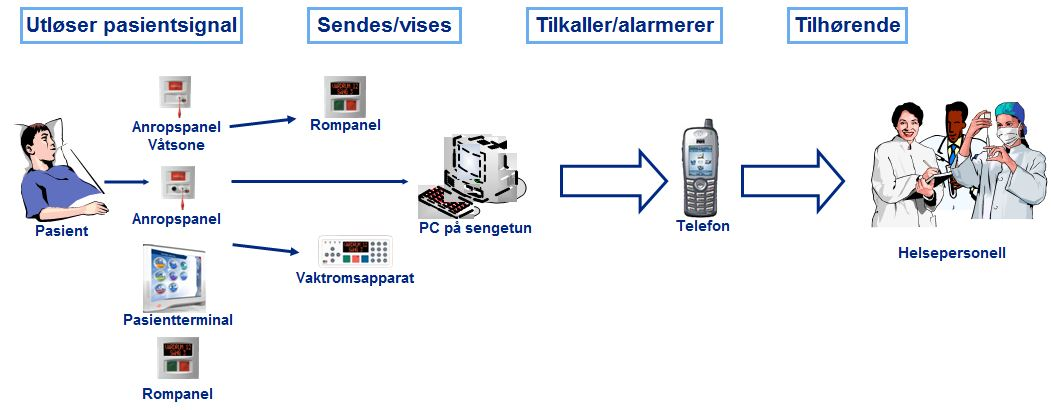
\includegraphics[scale=0.5]{alarmprosess.jpg}
\caption{Dette skjer ved utløst pasientsignal.}
\label{fig:detteskjer}
\end{figure}

\noindent
Sengepostene deles i sengetun, hvor hvert sengetun normalt har seks til åtte pasientrom. Sengetunet er en fysisk og funksjonell måte å organisere pasientrommene på, og for å sikre fleksibilitet og effektivitet ligger flere sengetun ved en sengepost etter hverandre i serie, som vist i figur \ref{fig:sengepost}. Signalsystemet kan til en viss grad konfigureres på en slik måte at sykepleiere på et sengetun kan motta pasientsignaler fra andre sengetun \citep{Aslaksen}.

\begin{figure}[H]
\centering
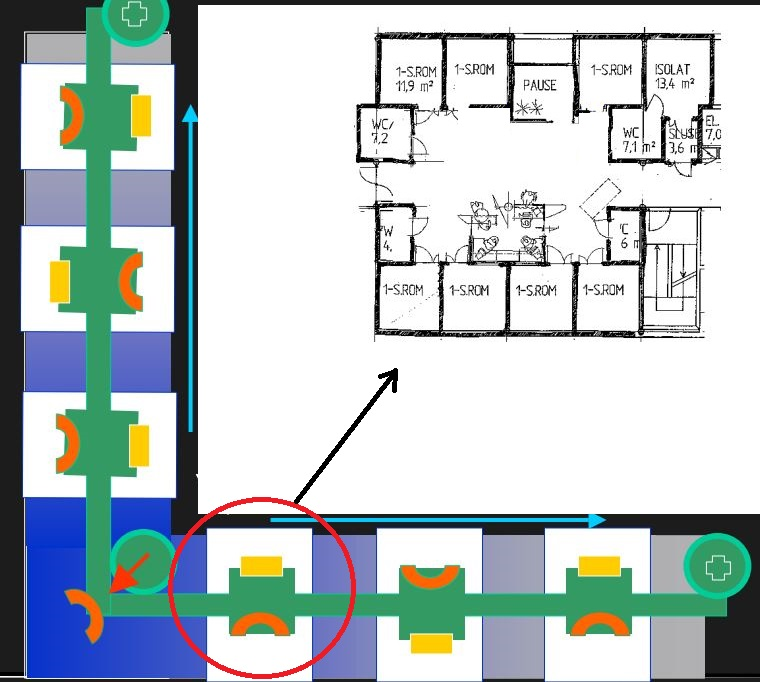
\includegraphics[scale=0.3]{sengepost.jpg}
\caption{Sengepost inndelt i sengetun \citep{Aslaksen}}
\label{fig:sengepost}
\end{figure}

\noindent
\textbf{FJERNE???} Varslingen av sykepleiere, gjør sykepleierene utsatt for eksterne avbrytelser i et allerede avbruddsdrevet miljø \citep{Klemets12}. Slike avbrudd i arbeidet kan ha både positive og negative effekter. Avbruddene kan eksempelvis gi informasjon som er nødvendig for koordinert og effektivt arbeid, og som gir bedre beslutningsgrunnlag for hvordan sykepleierne skal håndtere innkommende pasientsignaler. Slik systemet fungerer i dag er avbruddene uungåelig for å formidle denne informasjonen.
Sykepleierne vises som tilgjengelige i systemet selv når de er opptatt med oppgaver som gjør det lite ønskelig å motte pasientsignaler, som i disse tilfellene blir svært forstyrrende. \citet{KlemetsRedundancy} foreslår derfor at videre design av systemet bør tillate sykepleierene å sette seg selv som utilgjengelige. 

\section{Hensikt og foskningsspørsmål}
Motivasjonen for oppgaven har vært å kartlege sykepleiernes anvendlese av systemet, og identifisere forskjeller i bruk. Videre ønsket vi å svare på hva som kan være årsaker til at disse forskjellende har oppstått. 

\noindent
Da vi startet arbeidet med denne oppgaven var tanken at vi skulle se på hvordan systemet kunne endres for å bedre møte sykepleiernes behov. Etter første observasjonsrunde så vi imidlertid at en mer interessant vinkling ville være å se på hvordan systemet blir brukt forskjellig i, og mellom de forskjellige avdelingene, og hva de bakenforliggende årsakende til dette kan være. Dette resulterte i to forskningsspørsmål:

\begin{enumerate}
\item Hvordan brukes pasientsignalsystemet ved St.Olavs hospital forskjellig i, og mellom ulike avdelinger? 
\item Hvilke faktorer kan være årsak til disse forskjellene?
\end{enumerate}

\noindent
For å besvare disse spørsmålene har vi gjennomført både observasjoner og semistrukturerte intervjuer ved tre avdelinger ved St.Olavs hospital. Dataene fra disse innsamlingene ble så analysert og valg av relevent teori ble gjort i tråd med stegvis-deduktiv induktiv metode. Forskningsmetodene vi har anvendt er nærmere beskrevet i kapittel \ref{chp:metode}.

\section{Tidligere arbeid}
Slike tådløse systemer har vært subjekt for flere tidligere forskningsprosjekter. \citet{KlemetsRedundancy} ser på ansvarsfordeling og redundans av kunnskap blandt sykepleierne, og hvordan dette kan støttes av et slikt trådløst system. De peker på at konsekvensen med å innføre et slikt system i et allerede avbruddsdrevet miljø er en økning i antall forstyrrende avbrytelser. De foreslår mulige endringer for å minimere disse forstyrrelsene, blandt annet å implementere mulighet til å $"$gå av systemet$"$, og dermed ikke motta signaler. I \citep{klemets13} tar for seg sykepleiernes avgjørelsesprosess, og hvilke faktorer som påvirker denne. Det foreslåes derfor blandt annet å sende informasjon om anropet sammen med dette, samt visning av denne informasjonen på pasientterminaler og veggmonterte panel.

\noindent
Masteroppgaven \citep{Sletten09} er skrevet kort tid etter at det trådløse systemet ble innført på St.Olavs Hospital. Allerede her etterlyses en funksjon for å sette telefonen på $"$pause$"$ i situasjoner der sykepleierne ikke ønsker å bli forsyrret.
\citet{Rygh13} tar for seg forholdet pleiere og pasienter har til det trådløse pasientsignalsystemet, kontinuitet i pleie og hvilke muligheter som ligger i denne teknologien. Også her foreslåes muligheten for å sette telefonene i pausemodus for å redusere forstyrrelser. Både \citep{Rygh13} og \citep{Selseth12} trekker frem muligheten for å differensiere pasientsignalene på bakgrunn av pasientens behov. \citet{Selseth12} ser også på muligheten for pasientene å sende en slags tekstmelding til sykepleier om sine behov og en tidsramme for dette. Også mulighet for sykepleierene til å videresende disse melingene ble vurdert. 



\chapter{Casebeskrivelse}
\label{chp:case}
Utbyggingen av det nye universitetssykehuset i Trondheim, St.Olavs Hospital ble påbegynt i 2003 og sto ferdig sommeren 2013. Byggingen ble hovedsakelig delt i to byggefaser, hvor avdelingene flyttet inn i sine nye lokaler etter hver fase. Som en del av byggeprosjektet inngikk også det som da var Norges største, dyreste og mest kompliserte IKT-leveranse noensinne \citep{TU}. Pasientsignalsystemet var en del av denne leveransen, og ble utviklet spesielt for sykehuset. 

\noindent
Denne casebeskrivelsen omfatter en beskrivelse av de tre avdelingene, A1, A2 og A3, som har vært fokus for forskningsarbeidet. 

\noindent
Med det nye sykehuset ble utformingen av avdelingene endret. Avdelingene er nå delt i sengetun, hvor hvert sengetun normalt har seks til åtte pasientrom. Dette er en fysisk og funksjonell måte å organisere pasientrommene på, og for å sikre fleksibilitet og effektivitet ligger flere sengetun ved en sengepost etter hverandre i serie, som vist i figur \ref{fig:Bevegelse} og \ref{fig:AHL} \citep{Aslaksen, sykehuskart}. Sengetunene består av en arbeidsstasjon, nærlager, sengerom og toalett. Mellom tunene ligger støtterom som kjøkken og oppholdsrom for pasienter, medisinrom, skylle/avfallsrom og undersøkelsesrom. Et overordnet mål for en slik organisering er å redusere barrierer mellom pleier og pasient, bedre muligheter for overvåking av pasienter og redusere risiko for uønskede hendelser, noe som øker sikkerheten for pasientene \citep{Sintef-sengetun}.

\noindent
Avdeling A1 består av tre tun à seks sengerom, hvorav avdelingen har to luftsmitteisolat og seks kontaktsmitteisolat. Avdeling A2 består av tre tun à åtte sengerom. Avdeling A3 består av fire tun à åtte sengerom, fordelt på to etasjer.

\noindent
Avdelingene A2 og A3 er tydelig delt i sengetun (figur \ref{fig:Bevegelse} og \ref{fig:AHL}) mens avdeling A1 skiller seg fra de to andre da rommene er plassert i en lang gang uten tydelig avgrensede tun (figur \ref{fig:Ksenter}). Også utformingen av rommene på A1 skiller seg fra de andre da de har egen luftsluse mellom korridoren og hvert enkelt pasientrom.

\begin{figure}[H]
        \centering
        \begin{subfigure}[b]{1.0\textwidth}
        		\centering
				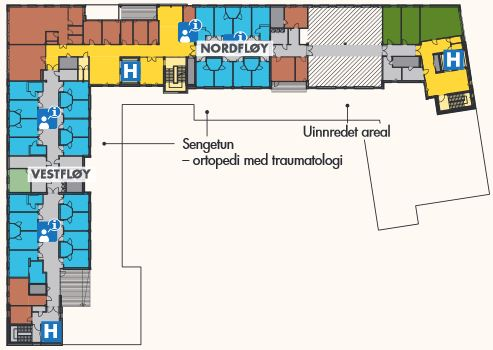
\includegraphics[scale=0.8]{bevegelse_6etg.jpg}
				\caption{Avdeling A2}
				\label{fig:Bevegelse}
        \end{subfigure}
        
        \begin{subfigure}[b]{1.0\textwidth}
        		\centering
				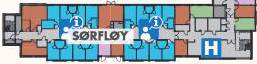
\includegraphics[scale=1.1]{AHL_5etg_sorfloy.jpg}
				\caption{Avdeling A3}
				\label{fig:AHL}
        \end{subfigure}
        
        \begin{subfigure}[b]{1.0\textwidth}
        		\centering
				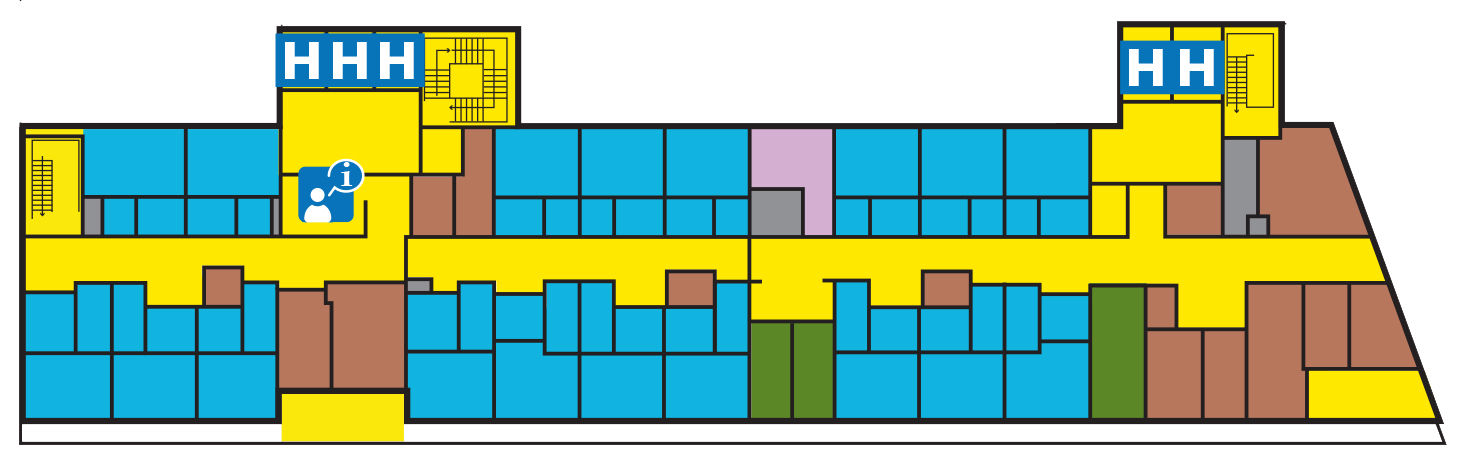
\includegraphics[scale=0.25]{Ksenter_6etg.jpg}
				\caption{Avdeling A1}
				\label{fig:Ksenter}		
        \end{subfigure}
        \caption{Plantegning av avdelingene. \citep{sykehuskart}.}
        \label{Plantegninger}
\end{figure}

\noindent
Arbeidstasjonene er utstyrt med PC'er og fungerer som en desentralisering av vaktrommet. På avdelingene A2 og A3 ligger denne som et senter på det åpne tunet ( figur \ref{fig:aapen_arbeidsstasjon}), mens den på avdeling A1 ligger på rekke med pasientrommene (figur \ref{fig:A1_arbeidsstasjon}).

\begin{figure}[H]
\centering
	\begin{subfigure}[b]{1.0\textwidth}
		\centering
		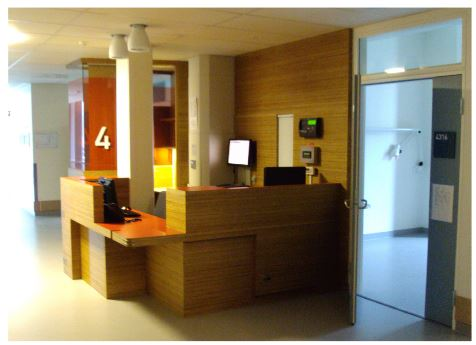
\includegraphics[scale=0.7]{aapen_arbeidsstasjon.jpg}
		\caption{Åpen arbeidsstasjon på sengetun slik den er på avdelingene A2 og A3 			\citep{sykehuskart}}
		\label{fig:aapen_arbeidsstasjon}
	\end{subfigure}
	
	\begin{subfigure}[b]{1.0\textwidth}
		\centering
		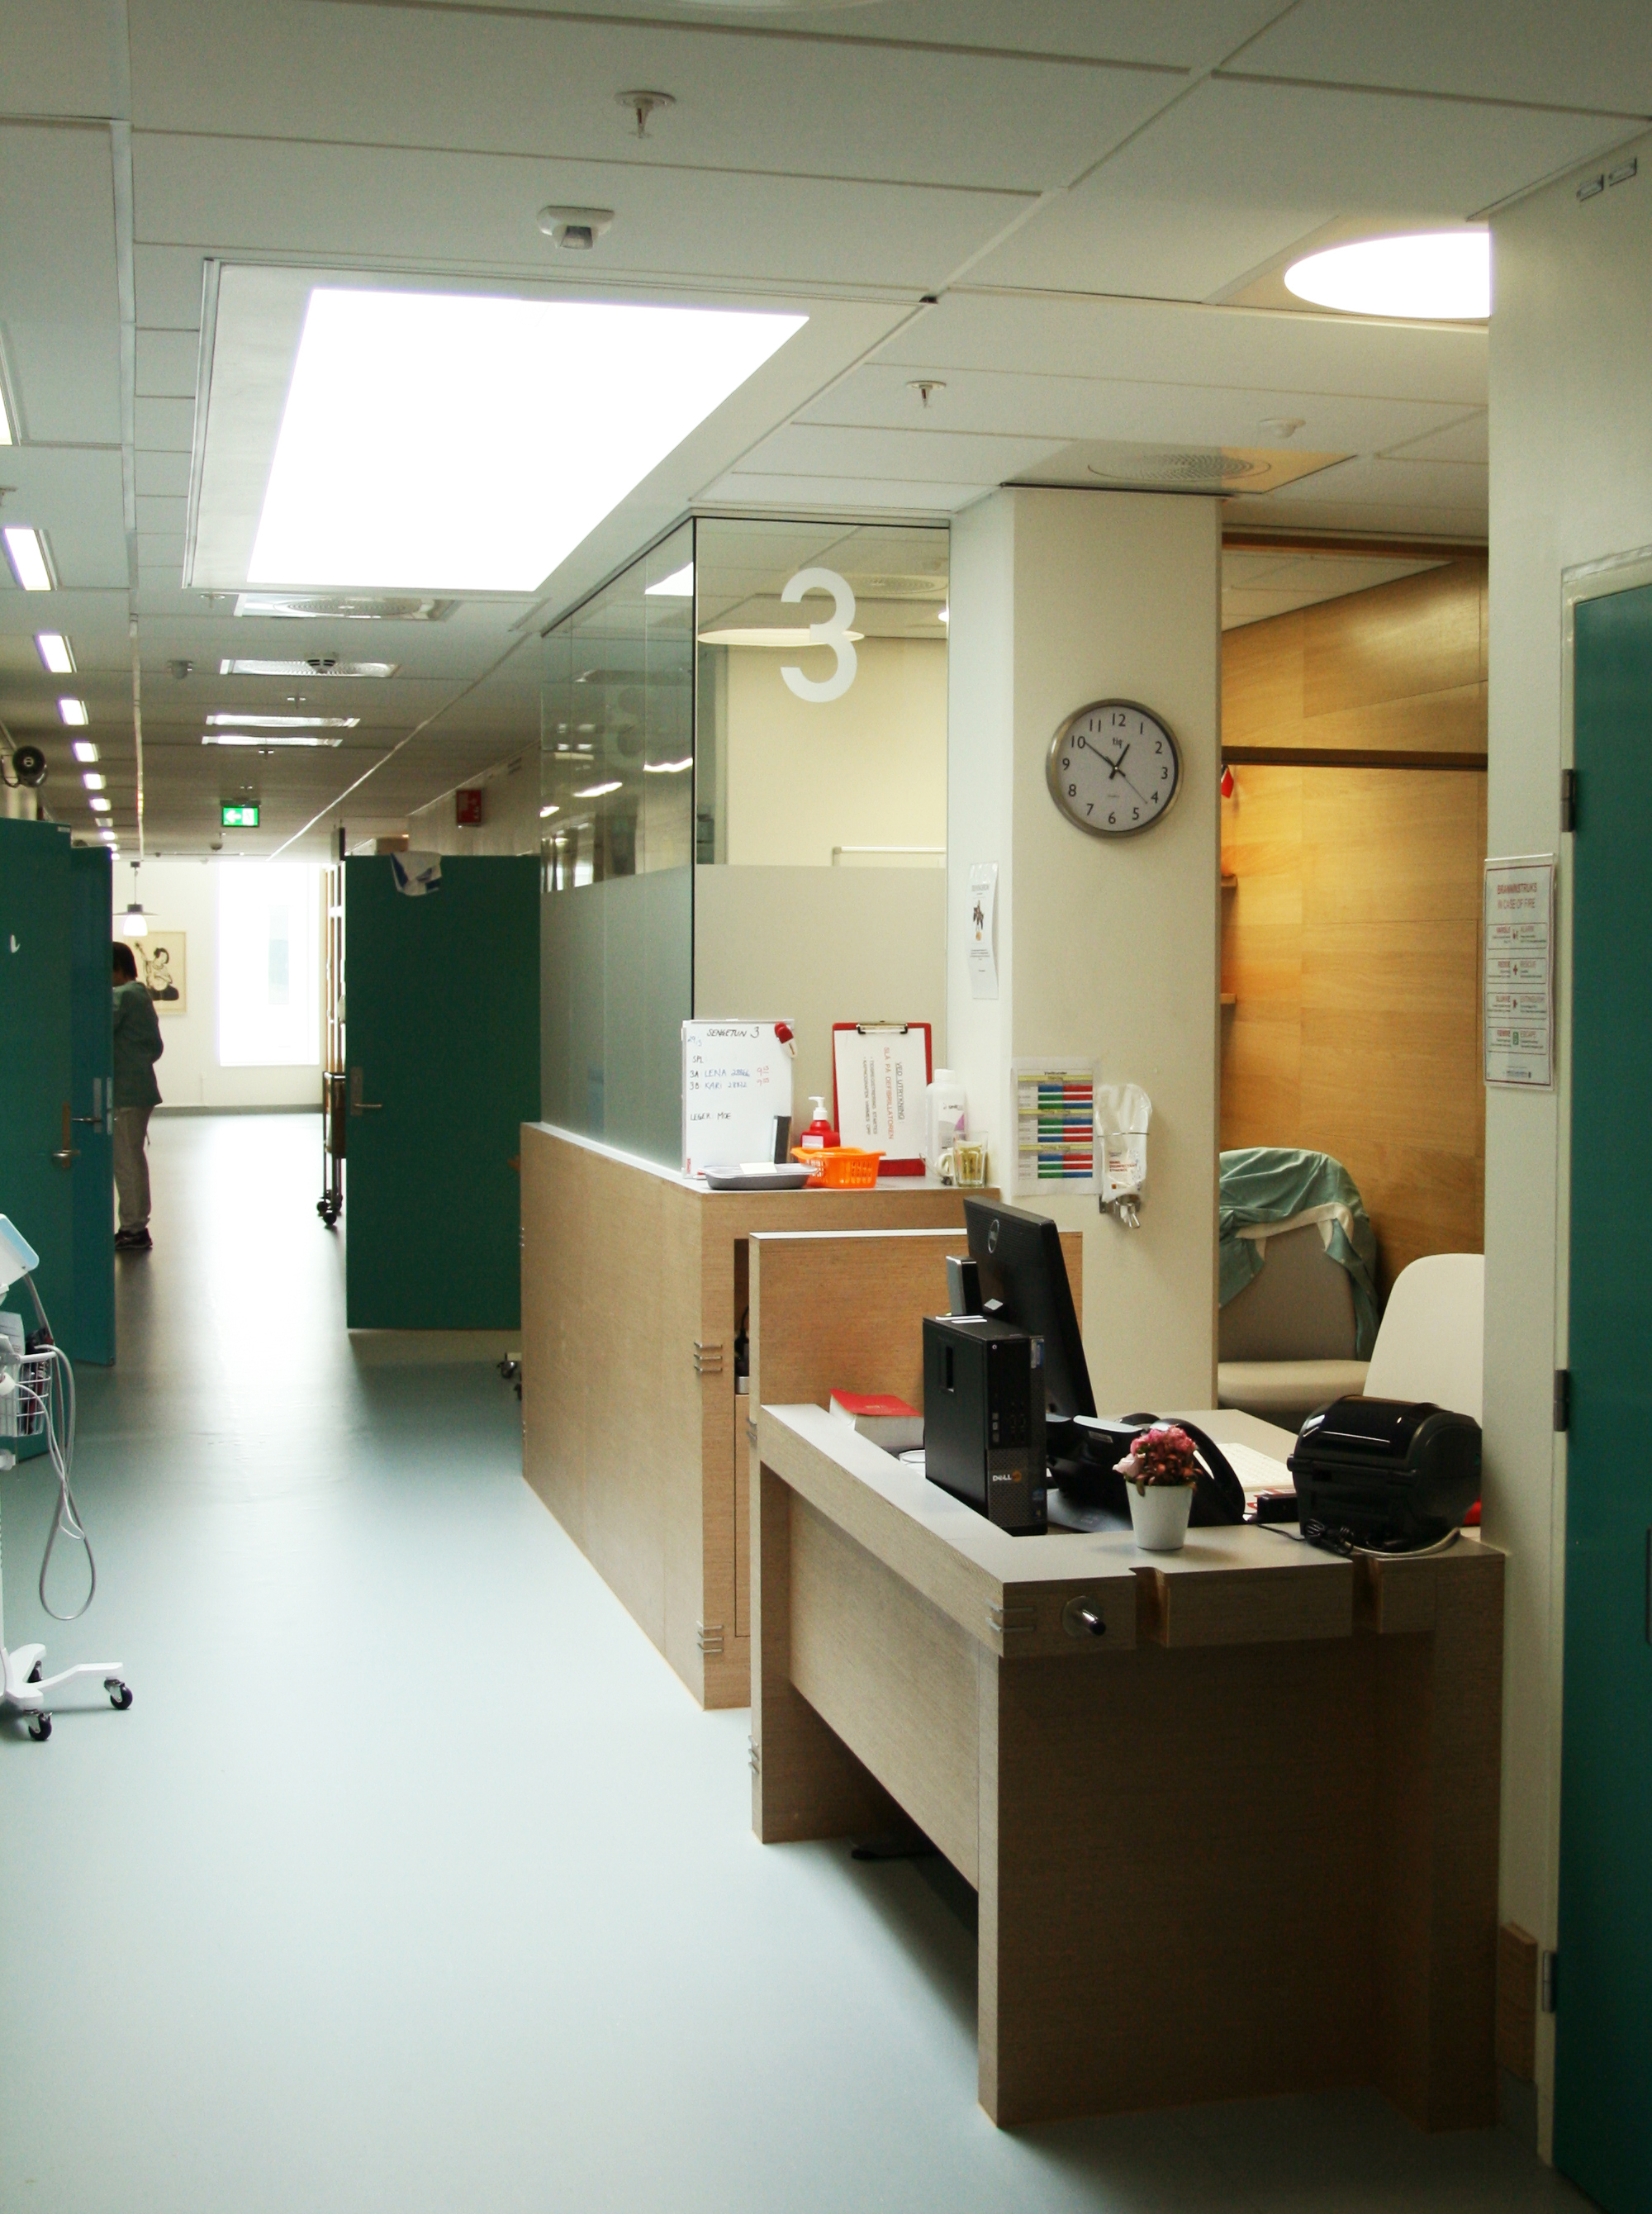
\includegraphics[scale=0.1]{A1_arbeidstasjon.jpg}
		\caption{Arbeidsstasjon på sengetun slik den er på avdeling A1 							\citep{sykehuskart}}
		\label{fig:A1_arbeidsstasjon}
	\end{subfigure}
\caption{Arbeidsstasjon på sengetun}
\label{fig:arbeidsstasjon}
\end{figure}

\section{System}
Pasientsignalsystemet består av et fast og et trådløst system. Det faste systemet består av anropspanel, rompanel og vaktromsapparat, mens det trådløse består av IP-telefoner, pasientterminaler og PC'er som kjører pasientsignalapplikasjon. En overordnet oversikt over varslingen av pasientsignal er illustrert i figur \ref{fig:detteskjer}. En mer detaljert beskrivelse finnes i vedlegg \ref{chp:appendix_dagenssystem}.

\begin{figure}[H]
\centering
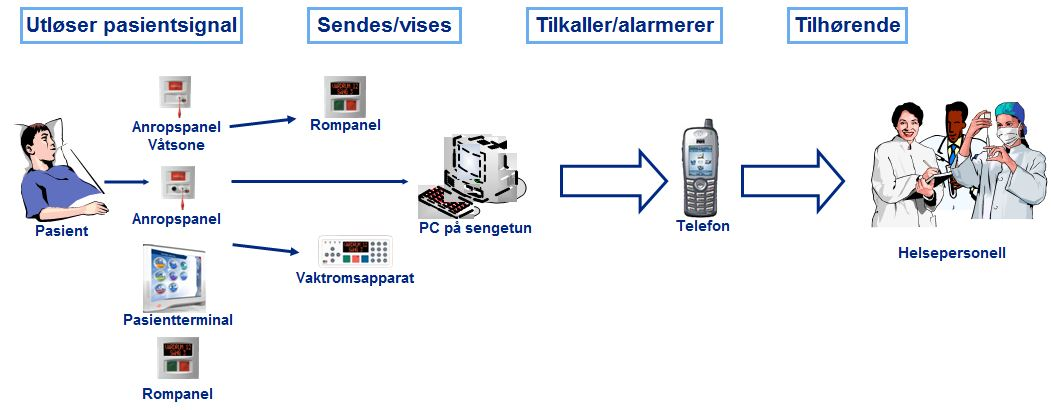
\includegraphics[scale=0.5]{alarmprosess.jpg}
\caption{Dette skjer ved utløst pasientsignal.}
\label{fig:detteskjer}
\end{figure}

\noindent
Hver arbeidsstasjon har en PC som kjører pasientsignalapplikasjonen, og gjennom denne kan sykepleierne registrere seg i en bemanningsplan (figur \ref{IMATISbemanningsplan}) og får oversikt over hvilke rom som er tilstedemarkert eller har pågående pasientsignaler og hasteanrop (figur \ref{IMATISpasientapplikasjon}). Applikasjonen gir pleierne mulighet til å selv påvirke hvordan pasientsignalene skal distribueres. Pleiere har mulighet til å registrere seg som primær og/eller disponibel på pasientrom og som disponibel på hele sitt eget eller andre tun. Det faste systemet er konfigurert i fysiske, kablede sløyfer som kobler sammen sengetun og gjør det mulig å motta varslinger fra andre tun på veggpanelene. I tilfeller hvor man ønsker å motta signaler fra tun som er koblet til andre sløyfer må pleierne motta disse på sin telefon, da dette kan konfigureres gjennom bemanningsplanen. Et utløst pasientsignal vil først varsles på telefon til den pleieren som er registrert som primær på det aktuelle rommet. Dersom signalet ikke blir godtatt vil det gå videre til disponible pleiere. Signalet vil fortsette i denne løkken til det blir besvart.

\begin{figure}[H]
\centering
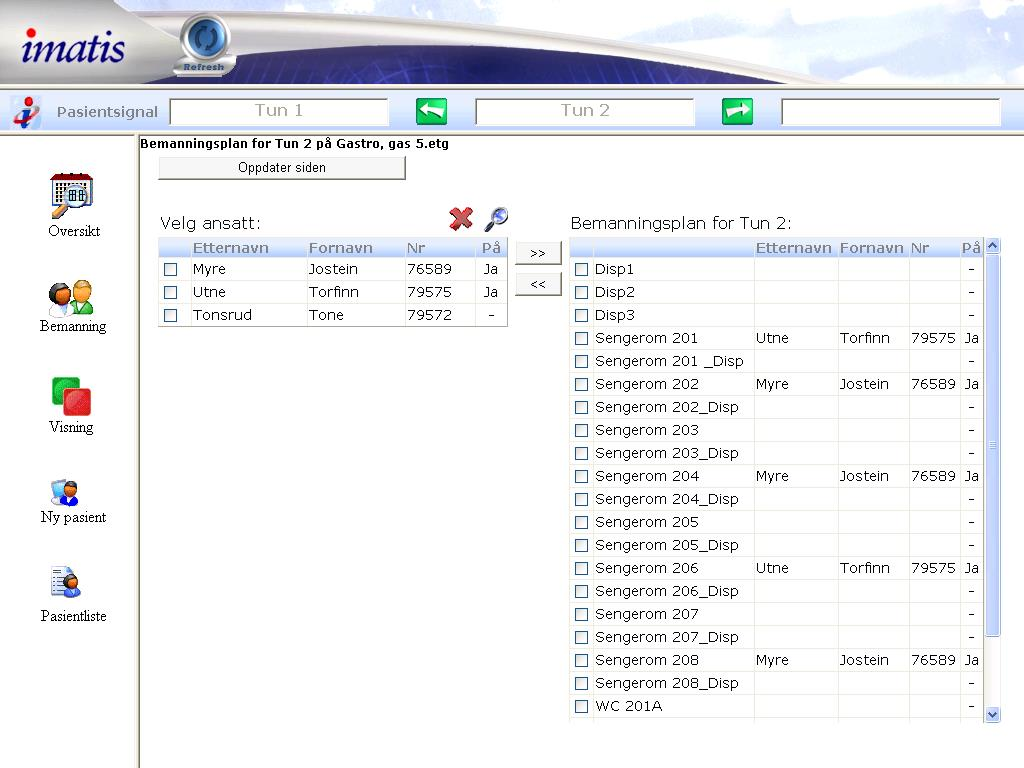
\includegraphics[scale=0.4]{bemanningsplan.jpg}
\caption{Bemanningsplan}
\label{IMATISbemanningsplan}
\end{figure}

\begin{figure}[H]
\centering
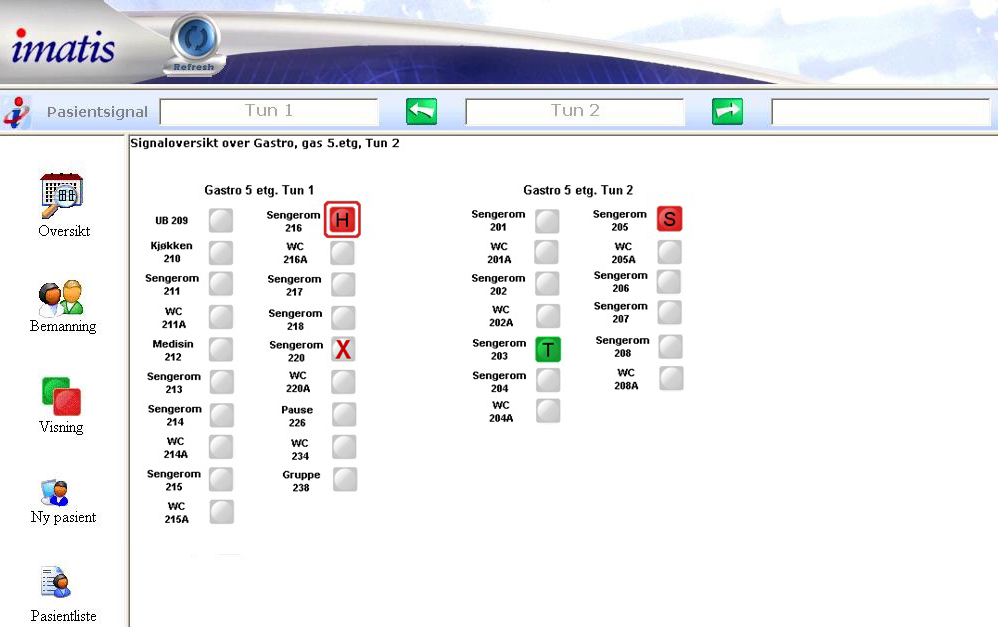
\includegraphics[scale=0.4]{pasientapplikasjon.jpg}
\caption{Signaloversikt på IMATIS-skjerm}
\label{IMATISpasientapplikasjon}
\end{figure}

\noindent
Pasientene kan tilkalle sykepleier ved å blant annet trekke i snoren på anropspanelet som er montert på veggen ved sengen. Signalet varsles da via vaktromsapparatet som henger synlig på sengetunet, via rompaneler på de pasientrom hvor sykepleiere er tilstedemarkert (denne markeringen gjøres ved at sykepleier trykker på den grønne knappen på rompanelet) og på telefonen til sykepleiere i henhold til bemanningsplanen (figur \ref{varslinger}). 

\begin{figure}[H]
        \centering
         \begin{subfigure}[b]{0.3\textwidth}
        		\centering
                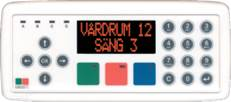
\includegraphics[scale=1.1]{vaktromsapparat.jpg}
                \caption{Vaktromsapparat}
                \label{rompanel}
        \end{subfigure}
        \begin{subfigure}[b]{0.3\textwidth}
        		\centering
                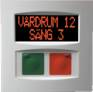
\includegraphics[scale=1.8]{rompanel.jpg}
                \caption{Rompanel}
                \label{rompanel}
        \end{subfigure}
          \begin{subfigure}[b]{0.3\textwidth}
        		\centering
                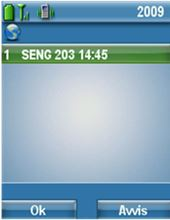
\includegraphics[scale=0.6]{signal_telefon.jpg}
                \caption{Telefon}
                \label{signal_telefon}
        \end{subfigure}      
        \caption{Varslinger av pasientsignal}
        \label{varslinger}
\end{figure}

\noindent
Ved et innkommende pasientsignal kan sykepleieren velge å godta eller avvise signalet på telefonen (figur \ref{signal_telefon}). Dersom pleieren velger å avvise signalet, eller ingen valg gjøres innen 15 sekunder, sendes signalet videre til neste pleier i henhold til bemanningsplanen. Dersom pleierne velger å godta signalet blir dette lagt i arbeidslisten på telefonen, og pleieren har 120 sekunder på seg til å tilstedemarkere seg på det aktuelle pasientrommet \citep{BrukermanualforPasientsignalogPasientsignalapplikasjon}. 

\noindent
Pleiere kan utløse hasteanrop i tilfeller hvor de har behov for assistanse. Dersom pasientrommet er tilstedemarkert gjøres dette ved å trykke på den røde knappen på rompanelet, hvis ikke må denne holdes inne i to sekunder \citep{BrukerveiledningforPasientsignal}.

\noindent
Der de samme signalene varsles på veggpanelene og på telefon fører en forsinkelse i det trådløse systemet til at signalet varsles tidligere på veggpanelene. Det foreligger desverre ingen tall på hvor stor forsinkelsen er. 

\noindent
Systemet skiller seg fra det som ble brukt tidligere, blant annet i at pasientsignal da kun ble varslet på paneler på vegg og på større paneler i taket (se figur \ref{takpanel}). Også knappen sykepleierne kunne bruke for å formidle behov for assistanse ble fjernet (figur \ref{assistanseknapp}). 

\begin{figure}[H]
        \centering
        \begin{subfigure}[b]{1.0\textwidth}
        		\centering
                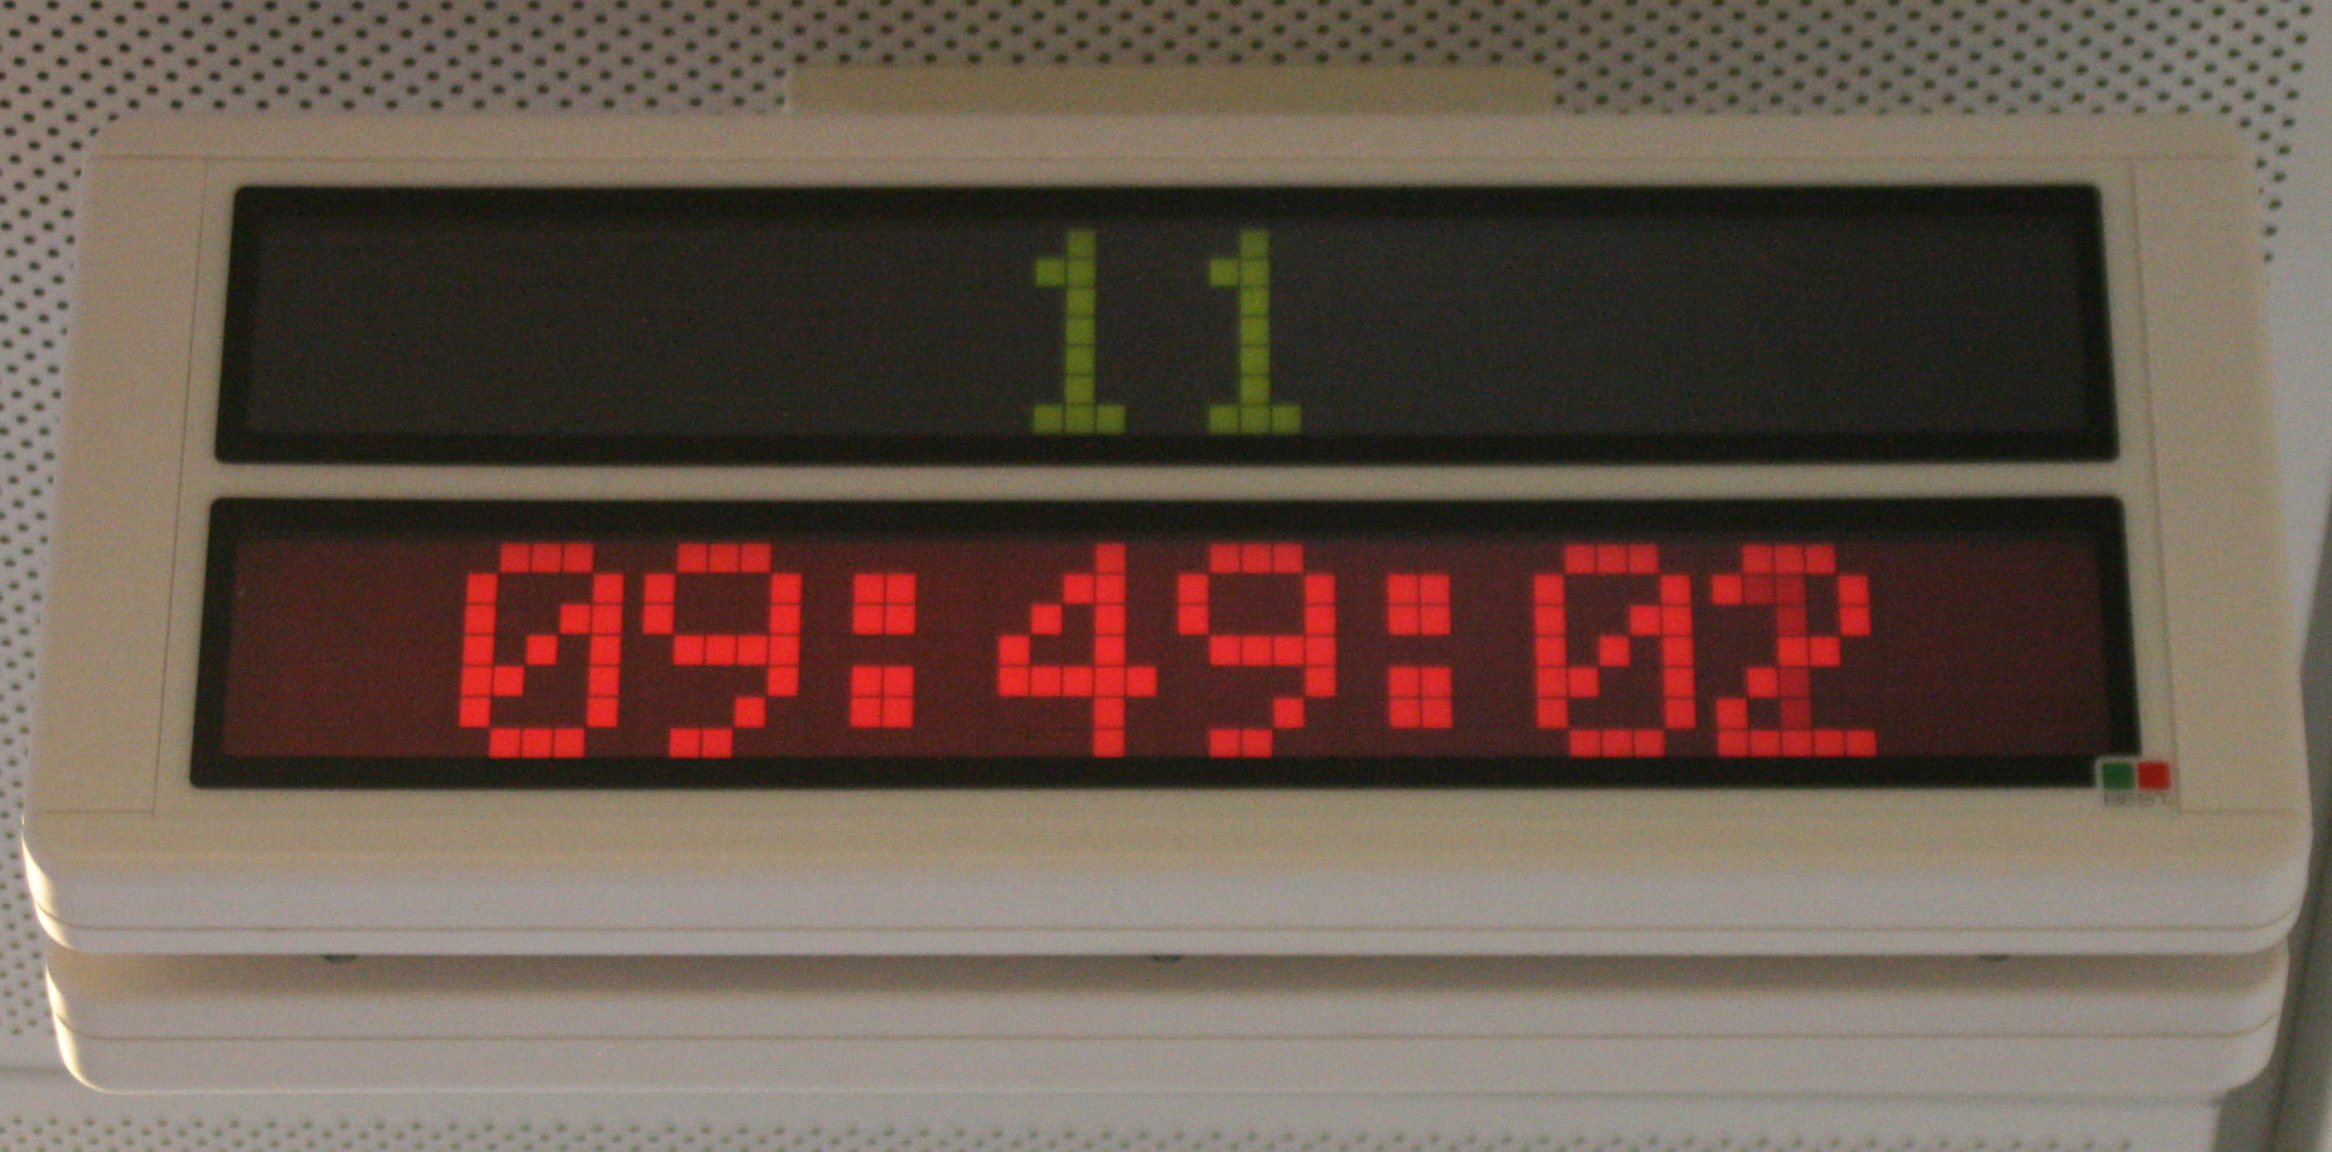
\includegraphics[scale=0.5]{takpanel.jpg}
                \caption{Panel i taket slik det var på det gamle sykehuset}
                \label{takpanel}
        \end{subfigure}
        
        \begin{subfigure}[b]{1.0\textwidth}
        		\centering
                
\includegraphics[scale=0.08]{assistanseknapp.jpg}
                \caption{Rompanel med egen knapp for assistansesignal}
                \label{assistanseknapp}
        \end{subfigure}
        \caption{Features ved det gamle sykehuset}
        \label{takass}
\end{figure}


\noindent
I forkant av innflyttingen fikk de ansatte opplæring, blant annet i hvordan det nye pasientsignalsystemet fungerte. Noen ansatte fikk mer omfattende opplæring og ble $"$superbrukere$"$ av systemet, med den hensikt å fungere som ambassadører for systemet, og hjelpe til med opplæring på avdelingene. Den første tiden etter at systemet var tatt i bruk var det også plassert $"$on site help desk$"$ på alle avdelinger for å svare på spørsmål og hjelpe til med bruk. I dag er det den enkelte avdeling som har ansvar for opplæring av sine nyansatte. 

\noindent
Ved innflyttingen i nytt sykehus var det meningen at alle skulle bruke telefonen til å motta pasientsignaler. Det var derimot noen avdelinger, deriblant avdeling A1, som viste sterk motstand og ikke ønsket å bruke telefonene til dette.
Høsten 2013 flyttet avdelingen på nytt inn i nye lokaler, og gikk i forbindelse med dette med på å bruke systemet slik det var tiltenkt i en prøveperiode på 14 dager. Etter denne prøveperioden gikk avdelingen likevel tilbake til å ikke motta pasientsignaler på telefon. 
I forbindelse med denne flyttingen fikk de også tilbake assistanseknappen (figur \ref{assistanseknapp}) de lenge hadde ønsket seg. Denne er plassert sammen med den grønne og røde knappen på panelet inne på pasientrommet. Disse signalene varsles med et annet signal enn vanlige pasientsignal og vises kun på veggpanelene og ikke i pasientapplikasjonen på IMATIS-skjermen.
\chapter{Teori}
\label{chp:teori} 

Vi vil i dette kapittelet se på teori som er relevant for vår forskning. Da vi har jobbet etter SDI-metoden (forklart nærmere i kapittel \ref{section:kvalitativ_analyse}) har funnene i aller største grad påvirket hvilken teori vi har fokusert på. Der teorien overlapper med den i vår prosjektoppgave \citep{Sund13} er teksten hentet derfra. 

\noindent
Siden midten av 80-tallet har det blitt forsket på hvordan datasystemer kan være til støtte for samarbeid og kommunikasjon mellom individer \citep{Rogers94}, hvordan mennesker samarbeider for å utføre arbeidsaktiviteter, og hvordan teknologi kan være til støtte for dette \citep{Ellis91}. Dette tverrfaglige området kalles CSCW, som er en forkortelse for det engelske $"$Computer-Supported Cooperative Work$"$. På norsk kan dette oversettes til $"$datastøttet samarbeid$"$ og defineres som PC-baserte systemer som støtter grupper av mennesker engasjert i en felles oppgave, eller med et felles mål, som gir et grensesnitt til det delte miljøet \citep{Ellis91}.

\noindent
Et typisk CSCW-system vil vanligvis bli brukt av et bredt spekter av brukere, med forskjellig bakgrunn, erfaringer og forhold til bruk av informasjonssystemer generelt, noe som gjør utviklingen av et slikt system svært kompleks. Desverre er det ikke uvanlig at beslutningstakere tar avgjørelser basert på hva slags funksjoner som vil være fordelaktig for brukere som dem selv, og dermed overser hva andre brukere kan ha nytte av. Funksjonalitet som lettet arbeidet for én gruppe brukere, kan gi merarbeid til en annen gruppe brukere. Det kan også være vanskelig å lære fra tidligere feil, da CSCW-systemer er svært komplekse og unike for hvert enkelt tilfelle, noe som vanskeliggjør evaluering i ettertid. Det er utfordrende å gjenskape miljø og forhold som er essensielle i den virkelige konteksten hvor et CSCW-system skal implementeres, i et laboratorium. Feltobservasjoner kan også gi et feilaktig inntrykk, da det kan være variasjoner avhengig av gruppesammensetning og miljømessige faktorer \citep{Berg99}.


\noindent
Det å utvikle et CSCW-system for helseomsorgen vil dermed kunne være en utfordrende prosess. Det er en konflikt mellom det flytende samarbeidet og de tilsynelatende uforutsette arbeidsoppgavene til sykepleiere, og den formelle, standardiserte og relativt stive funksjonaliteten til et informasjonsystem. Derfor er en av forutsetningene for et suksessfullt system i et slikt miljø, å ikke forsøke å erstatte denne 'rotetheten' med en rasjonalitet og strømlinjeform som ofte er vanlig for slike systemer. Verktøy som kun har forutbestemte sekvensielle trinn, eller som kun tillater gitte typer input vil derfor ikke fungere sammen med måten sykepleierne arbeider på, og som en følge av dette ikke overleve \citep{Berg99}.
\section{Sosioteknisk tilnærming}
\label{section:sosioteknisk}

Ikke alle informasjons- og kommunikasjonsteknologiske (IKT) systemer som introduseres i helseomsorgen er suksessfulle, og ifølge \citet{FITT} er det estimert at opp til 70\% av alle slike prosjekter feiler \citep{Coiera07}. Tradisjonelt sett er teknologien blitt designet først og menneskene tilpasset denne \citep{Appelbaum97}.
I dag må det ved design av tekniske systemer tas hensyn til at teknologien i stor grad er integrert i det sosiale domenet. Mennesker, vektøy og teknologi danner tilsammen det som kalles et \textit{$"$sosioteknisk system$"$} \citep{Coiera04}.
En sosioteknisk tilnærming til IKT-systemer forsøker å forstå hvordan mellommenneskelige aspekter og tekniske systemer påvirker hverandre \citep{Coiera04}, og hvordan interaksjonen mellom mennesker begrenser eller former interaksjonen mellom mennesker og teknologi \citep{Coiera07}. Menneskelig aktivitet er fleksibel, nyansert og kontekstualisert, og det er vanskelig å designe løsninger som støtter dette da tekniske systemer ofte er rigide og lite fleksible. Brukere skaper dermed kontinuerlig normer for bruk av et system som bidrar til å gjøre systemet mer fleksibelt \citep{Ackermann00}. \citet{Ackerman00} presenterer begrepet \textit{”sosioteknisk gap”}, og beskriver dette som det store skillet mellom de sosiale krav som stilles og hva som lar seg løse teknisk. Han argumenterer for at den sentrale utfordringen innen CSCW er å utforske, forstå og redusere dette gapet. \citet{Coiera04} poengterer at oppførselen til et sosioteknisk system fremkommer gjennom interaksjonen mellom komponentene, og flere komponenter vil dermed gjøre det vanskeligere å forutse utfallet av tilsynelatende enkle endringer. 

\noindent
Som beskrevet vil sosiale og tekniske systemer påvirke hverandre \citep{Coiera04}. Eksempler på at teknologien påvirker sosiale systemer blir synlig ved at innføring av teknologi i en ny setting ikke bare påvirke brukerne den er ment for, men også menneskene brukerne omgås. Eksempler på det motsatte, at sosiale systemer påvirker teknologien, er tydelig i tendensen vi ser i at mennesker i stadig større grad behandler datamaskiner og kommunikasjonsmedier som om det var mennesker, og en naturlig del av et sosialt system. I tillegg påpeker \citet{Coiera07} at brukernes forhold til teknologien i et slikt system vil bli tydelig påvirket av hva som skjer i det sosiale domenet. For det første vil villigheten til å bruke systemet avhenge av holdningen andre mennesker har ovenfor systemet. For det andre vil avgjørelsen om hvor mye kognitiv kapasitet vi til enhver tid tildeler teknologien være bestemt av hvem vi samhandler med på det sosiale planet på samme tid.

\noindent
Et annet perspektiv som trekkes frem av \citet{Coiera07} er mennerskers evne til å utvikle \emph{$"$workarounds$"$}, hvor en får teknologien til å oppføre seg på måter, og i settinger den ikke i utgangspunktet var ment for. Videre påpeker han at disse tilpasningene kan sees på som  implisitte signaler om et behov som ikke er dekket, og at å studere disse er en effektiv måte å identifisere styrker og svakheter ved eksisterende systemer og prosesser, og dermed forstå hva som må endres. 

\noindent
Avvik skjer ofte i arbeidsprosesser \citep{Ackermann00}, og workarounds defineres av \citet{Kobayashi05} som \emph{"informal temporary practices for handling exceptions to normal workflow$"$}. Oversatt til norsk betyr det $"$uformelle, midlertidige løsninger for å håndtere avvik fra normal arbeidsflyt$"$.
Workarounds kan være nødvendig når det oppstår akutte situasjoner hvor man ikke har nødvendige ressurser tilgjengelig, eller de kan oppstå som følge av sperrer i et system. Disse sperrene kan være tilsiktede, eller utilsiktede. \citet{Vogelsmeier08} beskriver workarounds som førstegrads problemløsing i den forstand at man lager mekanismer for å jobbe rundt problemer, uten å forsøke å løse den underliggende årsaken til at problemet oppsto. Dersom workarounds oppstår som konsekvens av at systemet er for rigid i forhold til sykepleierenes arbeidsmønster slik at systemet ikke støtter opp om arbeidet på en tilfredstillende måte, er dette svært uheldig. Dette kan i verste fall føre til livstruende situasjoner.

\noindent
En sosioteknisk tilnærming er altså ikke en liste med kriterier som må oppfylles for å sikre et suksessfullt system, men en metode som understreker at empirisk, kvalitativ innsikt og forståelse for den allerede eksisterende settingen teknologien skal passe inn i, bør være utgangspunktet for utvikling av IKT-systemer \citep{Berg99}. En slik tilnærming, med den ekstra dimensjonen som oppstår når andre mennesker konkurrerer om oppmerksomheten til et individ samtidig som det samhandler med teknologien, må ikke forveksles med teori om menneske-maskin interaksjon, som studerer hvordan individer jobber, og prossesserer informasjon når de ikke forstyrres av andre \citep{Coiera07}.

\noindent
Både \citet{Coiera07} og \citet{Berg99} trekker frem systemer i helseomsorgen som spesielt egnet for sosioteknisk analyse på grunn av sin svært komplekse natur. I følge \citet{Berg99} vil en sosioteknisk tilnærming være kritisk til systemer som forsøker å ta avsand fra den nødvendig rotete og $"$ad hoc$"$ måten helsearbeidere jobber på, gjennom IT-systemer med stor grad av standardisering og rasjonalisering av oppgave og arbeidsflyt.







\section{Implementering og adopsjon av nye IKT-systemer}
\label{sec:implementering}
Å investere i ny informasjonsteknologi vil kun lede til økt produktivitet dersom teknologien aksepteres og brukes \citep{Venkatesh99}. Ifølge \citet{Orlikowski92} har kognitive og strukturelle elementer betydelige implikasjoner for adopsjon, forståelse og tidlig bruk av et nytt CSCW-system. 

\subsection{Kognitive elementer}
\label{sec:kognitive_elementer}
Kognitive elementer betegner individers mentale modeller, som innebærer hvordan de tenker om verden, blant annet sin organisasjon, sitt arbeid og teknologi. Mens \citet{Berg99} og \citet{Ackermann00} understreker at brukere ofte har ulik kunnskap og bakgrunn, påpeker \citet{Orlikowski92} at brukere med felles faglig bakgrunn, arbeidserfaring og regelmessig interaksjon ofte fører til at en gruppe deler felles antagelser og verdier. Dersom ny teknologi skiller seg fra den som er brukt tidligere kreves en endring i brukernes mentale modell for at de skal forstå hvordan de skal interagere med den nye teknologien på en effektiv måte. Hvordan brukere endrer sine mentale modeller for å tilpasse seg ny teknologi avhenger av typen og mengden informasjon de mottar, og hvilken opplæring de får. Hvis brukergruppen har en dårlig eller feilaktig forståelse av de unike og nye egenskapene til en ny teknologi vil de kunne motsette seg å bruke den, eller velge å ikke integrere den i sitt arbeid. Informasjon og opplæring er derfor sentralt for å få brukerne til å forstå teknologiens muligheter og nytte \citep{Orlikowski92}. I tråd med TAM\footnote{Technology Acceptance Model} vil et individs ønske om å bruke et system avhenge av to faktorer: (1) opplevd nytte, definert som i hvilken grad en person mener at bruk av et system vil øke sin jobbytelse, og (2) oppfattet $"$ease of use$"$, definert som i hvilken grad et system oppleves som enkelt å bruke \citep{Venkatesh00}. Opplæring er derfor essensielt for at brukere skal oppfatte ny teknologi som enkel å bruke, som igjen fører til at teknologien aksepteres og brukes videre \citep{Venkatesh99}.

\subsection{Strukturelle elementer}
\label{sec:strukturelle_elementer}
Strukturelle elementer betegner belønningssystemer, retningslinjer, arbeidspraksis og normer som formes av menneskene i organisasjonen. I en organisasjon kan individer og grupper ha ulike mål, ulik kunnskap og bakgrunn \citep{Ackermann00}. Dersom teknologien ikke er tilpasset organisasjonens strukturelle elementer, vil den sannsynligvis ikke skape effektiv samhandling uten at disse endres. \citet{Orlikowski92} viser et eksempel fra et stort tjenestefirma $"$Alpha Solutions$"$ (pseudonym), som har implementert applikasjonen $"$Notes$"$. Notes støtter kommunikasjon, koordinasjon og samarbeid innen organisasjonen, og inkluderer blant annet e-post og mulighet for diskusjonsforum og lignende. En av utfordringene ved implementeringen av Notes var at firmaet hadde en konkurransepreget kultur, hvor ansatte i stor grad jobbet selvstendig og ikke ønsket å dele informasjon. Denne individualismen støttet ikke samarbeid og deling av kunnskap, og sto dermed i kontrast til de underliggende forutsetningene for CSCW-systemet. 


\noindent
For sykepleiere kan et strukturelt element være hvordan de organiserer ansvar og oppgaver. Dette kan gjøres på ulike måter og \citet{Rygh13} presenterer primærsykepleie og teamsykepleie som modeller for dette. Førstnevnte deler oppgavene inn i kategorier som medisinering og sårstell. Hver sykepleier får deretter sine oppgaver som de har ansvar for den aktuelle vakten. På denne måten vil sykepleierne som team tilsammen utføre alle oppgaver. Teamledere koordinerer omsorgen utført av teamet og har, i samarbeid med avdelingsleder, ansvar for pasientbehandling og kommunikasjon med annet helsepersonell. I primærsykepleie tildeles ansvar for pasientene til individuelle sykepleiere. Primærsykepleier har ansvar for koordinering av omsorg og pleie for et lite antall paseinter fra innleggelse til utskrivelse, uten å måtte gjøre alle oppgaver knyttet til dette. 

\noindent
Forskning viser til at innføring av primærsykepleie i stor grad kan gjøre pleierne mer autonome i sitt arbeid, og også mer pasientorientert. Nyere forskning viser imidlertid at avdelinger ofte er organisert på måter som tar i bruk egenskaper fra de forskjellige modellene. Et eksempel på dette er modulær sykepleie som er organisert rundt relativt små geografiske grupperinger av pasienter, og hvor pleiepersonellet har ansvar for den totale omsorgen, og distribuerer oppgaver innenfor teamet \citep{Rygh13}.

\subsection{Tilpasning og interaksjon mellom elementene i et sosioteknisk system}
\label{sec:tilpasning}
\citet{Harrison} påpeker at implementering av ny IT\footnote{Informasjonsteknologi} i helsesektoren ofte medfører uforutsette og uønskede konsekvenser, noe som kan undergrave gitte praksiser og i verste fall være en risiko for pasientsikkerheten. Ofte vil helsepersonell skylde på teknologien for at slike konsekvenser og implementeringsfeil oppstår, til tross for at det i flere tilfeller er det sosiotekniske samspillet som har feilet. En vanlig feiltolkning er at problemer som ligger i samspillet mellom bruker og oppgave blir tillagt teknologien. Et eksempel på dette er dersom innføringen av et nytt IT-system gir brukerne flere dokumentasjonssoppgaver. Ofte vil det nye systemet få skylden for dette, mens problemet ikke nødvendigvis ligger i teknologien i seg selv, men i brukernes misnøye med oppgaven \citep{FITT}.

\noindent
\citet{Harrison} deler det sosiotekniske systemet i ny teknologi, arbeidsmønstre, helsepersonell og organisasjon. Samspillet mellom disse elementene innebærer komplekse interaksjoner, og kan føre til svært ulik bruk selv av identiske systemer. Eksempler på slike interaksjoner er:

\begin{itemize}
\item Ny IT endrer det eksisterende sosiale systemet, deriblant arbeidsmønstre, kommunikasjon og relasjon mellom helsepersonell. Teknologien kan eksempelvis føre til at helsepersonell må bruke mer tid på dokumentasjon enn tidligere, eller en reduksjon i kommunikasjonen ansikt-til-ansikt.
\item Manglende tilpasning av IT til den fysiske settingen hvor den skal tas i bruk kan medføre bruk og workarounds som har negative effekter på sikkerhet, kvalitet og effektivitet. Teknologien kan eksempelvis være plassert slik at den er problematisk å aksessere eller flytte.
\item Fortolkninger og tilpasninger av ny IT vil ofte føre til praksiser som skiller seg fra tenkt bruk. Disse avvikene oppstår fordi det opprinnelige designet ikke reflekterer de eksisterende arbeidsmønstre og sosiale relasjoner, og workarounds oppstår som resultat av dette. 
\item Som et resultat av at brukere gjør lokale tilpasninger som skiller seg fra tenkt bruk kan utviklere og ledere være tvunget til å gjøre endringer i teknologien.
\end{itemize} 

\noindent
For å lettere kunne analysere og identifisere de sosiotekniske faktorene som påvirker innføringen av nye IT-applikasjoner og -systemer, deler \citet{FITT} settingen hvor sysstemet skal brukes inn i de tre objektene individ, oppgave og teknologi. Hensikten er å se på samspillet mellom objektene (og deres egenskaper) og hvordan de passer sammen, ikke objektene i seg selv, for dermed å kunne peke på hvilke faktorer det er som hindrer optimal utnyttelse av den teknologien. De tre objektene innehar ulike egenskaper som kan være tilstede i større eller mindre grad. For et individ kan disse blant annet være IT-kunnskap, motivasjon, åpenhet for endringer i arbeidsmåte og team-kultur. For en oppgave kan det være organisering av oppgavene som skal gjennomføres og oppgavenes grad av kompleksitet. Teknologi kan ha egenskaper som stabilitet og brukbarhet, funksjonalitet og tilgjengelig teknisk infrastruktur. Dersom objektene mangler, eller har lite utviklede egenskaper som er nødvendige for et optimalt samspill, kan man direkte påvirke disse. Et eksempel er manglende IT-kunnskap blant brukerne (individ), hvor opplæring av ansatte kan øke tilstedeværelsen av denne egenskapen. Siden dette er tiltak som påvirker objektene, har det en indirekte påvirkning på samspillet mellom dem. 

\subsection{Workarounds}
\label{sec:workarounds}
Menneskelig aktivitet er fleksibel, nyansert og kontekstualisert, og det er vanskelig å designe løsninger som støtter dette da tekniske systemer ofte er rigide og lite fleksible. Brukere skaper derfor kontinuerlig normer for bruk av et system som bidrar til å gjøre systemet mer fleksibelt. Dermed kan systemer brukes på måter som utviklerne ikke har forutsett \citep{Ackermann00}. Ved å få teknologi til å oppføre seg på måter, og i settinger den ikke i utgangspunktet var ment for oppstår det som kalles $"$workarounds$"$. Slike tilpasninger kan sees på som implisitte signaler om behov som ikke er dekket, og at å studere disse er en effektiv måte å identifisere styrker og svakheter ved eksisterende systemer og prosesser, og dermed forstå hva som må endres \citep{Coiera07}. 

\noindent
Workarounds defineres av \citet{Kobayashi05} som \emph{"informal temporary practices for handling exceptions to normal workflow$"$}. Oversatt til norsk betyr det $"$uformelle, midlertidige løsninger for å håndtere avvik fra normal arbeidsflyt$"$. Slike midlertidige løsninger kan være nødvendig når det oppstår akutte situasjoner hvor man ikke har nødvendige ressurser tilgjengelig, eller de kan oppstå som følge av sperrer i et system. Disse sperrene kan være tilsiktede, eller utilsiktede. \citet{Vogelsmeier08} beskriver workarounds som førstegrads problemløsing i den forstand at man lager mekanismer for å jobbe rundt problemer, uten å forsøke å løse den underliggende årsaken til at problemet oppsto. Dersom workarounds oppstår som konsekvens av at systemet er for rigid i forhold til sykepleierenes arbeidsmønster slik at systemet ikke støtter opp om arbeidet på en tilfredstillende måte, er dette svært uheldig. Dette kan i verste fall føre til livstruende situasjoner.

\noindent
Det å utvikle et CSCW-system for helseomsorgen kan dermed være en utfordrende prosess. Det er konflikt mellom det flytende samarbeidet og de tilsynelatende uforutsette arbeidsoppgavene til sykepleiere, og den formelle, standardiserte og relativt stive funksjonaliteten til et informasjonsystem. En av forutsetningene for et suksessfullt system i et slikt miljø er derfor å ikke forsøke å erstatte denne $"$rotetheten$"$ med en rasjonalitet og strømlinjeform som ofte er vanlig for slike systemer. Verktøy som kun har forutbestemte sekvensielle trinn, eller som kun tillater gitte typer input vil derfor ikke fungere sammen med sykepleiernes arbeidsmåter, og som en følge av dette ikke overleve \citep{Berg99}.
Ifølge \citet{Berg99} vil en sosioteknisk tilnærming være kritisk til systemer som forsøker å ta avsand fra den nødvendig rotete og $"$ad hoc$"$ måten helsearbeidere jobber på, gjennom IT-systemer med stor grad av standardisering og rasjonalisering av oppgave og arbeidsflyt.

\noindent
Det å utvikle gode CSCW-systemer kan være svært utfordrende. I tillegg til å måtte passe en organisasjons kognitive og strukturelle elementer, vil mangfoldet av brukere innebære individuelle erfaringer og holdninger til bruk av et informasjonssystem. Videre kan det være vanskelig å lære fra tidligere feil da slike systemer er svært komplekse og unike for hvert enkelt tilfelle, noe som vanskeliggjør evaluering i ettertid. Det er i tillegg utfordrende å gjenskape miljø og forhold som er essensielle i den virkelige konteksten hvor systemet skal implementeres i et laboratorium \citep{Berg99}.

\subsection{Motstand}
\label{sec:motstand}
Tidligere studier har vist at motstand er et mangfoldig og vedvarende fenomen, og kan enkelt forklares som alt ansatte gjør som ledelsen ikke vil de skal gjøre, og alt de unnlater å gjøre som ledelsen ønsker de skal gjøre \citep{Timmons03}.
 
\noindent
Når vi ser på motstand mot endring er det viktig å identifisere og forstå hva som er årsaken til motstanden \citep{Lapointe05}. \citet{Timmons03} påpeker at årsakene til motstand oppstår i grensesnittet mellom systemet og eksisterende arbeidsmetoder, som også er i tråd med en sosioteknisk tankegang. \citet{Jacobsen12} trekker blant annet frem faglig uenighet rundt nødvendigheten av endringen eller valg av løsning, frykt for det ukjente og usikkerheten endringen medfører og ekstraarbeid som mulige årsaker til motstand.
 
\noindent
Motstand synliggjøres hovedsakelig gjennom motstandernes adferd, og \citet{Lapointe05} klassifiserer motstand i fire nivåer basert på dette.
 
\begin{itemize}
\item Apati inkluderer passivitet, mangel på interesse og distanse fra endringen.
\item Passiv motstand inkluderer forsinkelser, unnskyldninger og lite villighet for endring i arbeidsmåter.
\item Aktiv motstand tar blant annet i bruk ytringer av opposisjonerende meninger, dannelse av koalisjoner og delvis eller total nekt av bruk av systemet.
\item Aggressiv motstand kan innebære intern strid, trusler, streik, boikott og sabotasje, og søker å være forstyrrende eller destruktiv.
\end{itemize}
 
\noindent
Det vanlige fokuset i forskning på menneske-maskin interaksjon er brukere av systemet, og i tilfeller hvor ikke-brukere har vært av interesse, er disse gjerne identifisert som potensielle brukere. \citet{Satchell09} understreker at dette ikke gjelder alle, og de trekker frem misnøye med systemet, uttrykt gjennom kun delvis bruk av dette, og aktiv motstand som former for ikke-bruk.
 
\noindent
Motstand oppfattes ofte som utelukkende negativt, og de som motsetter seg en endring sees ofte på som gammeldags \citep{Jacobsen12}. Brukerne blir av mange delt inn i gode og  dårlige brukere, henholdsvis de som adopterer og bruker systemet slik det var tenkt, og de som ikke omfavner systemet \citep{Satchell09}. Dette skjuler det faktum at motstand i mange tilfeller bør sees som noe positivt, i form av kritiske innvendinger til behovet for endring og valg av løsning. Fravær av motstand \textit{kan} bety at alle er enige og går helhjertet inn for den nye løsningen, men det kan også bety at de ansatte er uinteressert i hvordan det går med organisasjonen \citep{Jacobsen12}. På samme måte er ikke ikke-bruk fravær av noe eller et tomrom, men ofte heller aktivt, meningsfullt, motivert, overveid, strukturert og produktivt \citep{Satchell09}
 

\section{Avbrudd}
\label{sec:avbrudd}

\emph{Eksterne avbrytelser} refererer til situasjoner hvor en ekstern hendelse fører til en forstyrrelse i prosessen med å fullføre en oppgave \citep{Harr07}.

\subsection{Dualiteten ved avbrudd}
\citet{Grundgeiger09} skiller mellom \emph{gode} og \emph{dårlige} avbrudd, og hevder disse bør sees i sammenheng med hvilke effekter de har. Eksempler på positive effekter er awareness om perifer informasjon, øyeblikkelig kommunikasjon og tilgang til viktig informasjon. Avbryter opplever å få en umiddelbar bekreftelse på at informasjonen er mottatt og kan dermed avlaste arbeidsminnet, mens den som blir avbrutt kan oppleve en negativ effekt, eksempelvis at den kognitive kapasiteten overskrides, forsinkelse i eget arbeid, stress og frustrasjon. Samtidig kan avbruddet ha en positiv effekt dersom den som blir avbrutt mottar en alarm om en pasients alvorlige tilstand, eller annen ønsket informasjon.


\subsection{Avbruddshåndtering}
Gitt denne dualiteten, kan avbruddshåndtering sies å ha to mål: (1) redusere de negative effektene, og (2) utnytte de positive effektene ved avbrudd. \citet{Grandhi10} gir fire teknikker for avbruddshåndtering:
\begin{enumerate}        
\item Forebygging - bruk av funksjoner som forebygger eller blokkerer innkommende avbrytelser, dette gjøres ofte enkelt ved å for eksempel skru av mobilen for en periode. En annen strategi er å kontrollere timingen til avbruddet, eller å kun tillate avbrytelser som er relevant for den oppgaven man utfører. Dette krever at awareness-informasjon er tilgjengelig, slik at timingen kan justeres for å minske den negative effekten ved avbruddet.

\item Fraråding - bruk av funksjoner som fraråder avbrytelser å oppstå, dette skjer ofte ved at man gir informasjon til avbryter om tilgjengeligheten til den man ønsker å avbryte. 

\item Modifiserte varslinger - bruk av funksjoner som modifiserer hvordan individer varsles om innkommende anrop. Ved bruk av ulike modaliteter som lyd, vibrasjon og lys, kan man minimere interferensen mellom perseptuelle og kognitive prosesser involvert i avbruddshåndtering og oppgaveytelse \citep{Harr07}.

\item Forhåndsvisning - bruk av funksjoner som gir informasjon om selve avbrytelsen som den avbrutte selv kan reflektere over.   
\end{enumerate}

\noindent
\textbf{FJERNE????}
Forskere som arbeider innen \emph{interruption impact reduction}-paradigmet for avbruddshåndtering fokuserer på hvordan avbrytelser påvirker oppgaveytelse. Timing, frekvens, lengde og relevans til nåværende aktivitet eller oppgave er faktorer som påvirker de potensielle negative effektene avbruddet kan forårsake \citep{Grandhi10, Harr07}.
Målet er dermed å redusere avbruddenes negative effekt på oppgaveytelsen, og de aktuelle teknikkene for å gjøre dette er forebygging, fraråding og modifikasjon. Disse teknikkene baserer seg på den lokale konteksten til den som avbrytes. Den lokale konteksten er sammensatt av: (1) kognitiv kontekst, den kognitive eller mentale arbeidsmengden individet opplever ved gjeldende oppgave, og (2) sosial kontekst, hvor individet befinner seg og hvem som er tilstede. 
 
\noindent
\citet{Harr07} presenterer fler aspekter knyttet til sosial kontekst, blandt annet lokasjonsbasert forstyrrelse og indirekte forstyrrelse.

\noindent
Avbrudd kan ha effekter på andre mennesker som befinner seg på samme lokasjon som den som blir avbrutt. Dette illustreres i figur \ref{collateral}, hvor interaksjonen mellom aktør D (avbryter) og aktør B (den som avbrytes) også påvirker aktører A og C.
\begin{figure}[H]
\centering
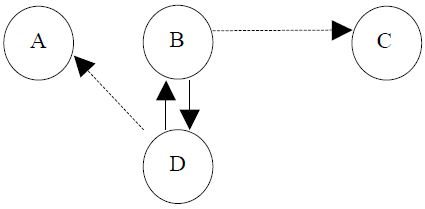
\includegraphics[scale=0.5]{collateral.jpg}
\caption{Lokasjonsbasert forstyrrelse}
\label{collateral}
\end{figure}

\noindent
Aktører B og C må ikke nødvendigvis kommunisere direkte, men aktør C kan være avhengig av tiden, innholdet og kvaliteten aktør Bs oppgave resulterer i. Dermed kan en forstyrrelse av aktør B også indirekte forstyrre aktør C.
\begin{figure}[H]
\centering
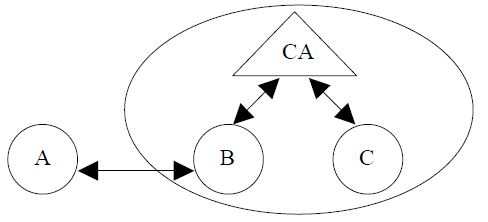
\includegraphics[scale=0.5]{dropball.jpg}
\caption{Samarbeid og avbrudd - indirekte forstyrrelse}
\label{indirekte}
\end{figure}

\noindent
\textbf{FJERNE????}
Forskere som arbeider innen \emph{interruption value evaluation}-paradigmet tar utgangspunkt i at ikke alle avbrudd er dårlige, og at de ikke bør evalueres kun avhengig av hvordan de påvirker lokal kontekst, men også avhengig av hvor stor nytte de har. Målet er dermed å optimalisere individets beslutningstakingsprosess om hvordan han skal respondere på avbruddet. Den mest aktuelle teknikken for avbruddshåndtering vil derfor være forhåndsvisning av informasjon om avbruddet, hvem det er fra og hva det handler om, slik at individet selv kan reflektere over hvordan han/hun skal respondere basert på sin lokale kontekst. Dermed vil det \citet{Grandhi10, Harr07} kaller relasjonell kontekst være en del av avbruddskonteksten. Denne defineres som alle aspekter mellom den som avbryter og den som blir avbrutt, hvilken relasjon de har, hva avbruddet dreier seg om og deres tidligere interaksjonsmønstre, i likhet med det \citet{Harr07} kaller mellommenneskelige relasjoner.

\subsection{Utfordringer}
\citet{Harr07} påpeker tre fundamentale utfordringer ved avbruddshåndtering: (1) fare for å miste informasjon, (2) mindre privatliv og (3) utsettelse av oppgaver. For hver situasjon må individer finne den optimale balansen mellom isolasjon og tilgjengelighet, åpenhet og privatliv, og direkte eller utsatt håndtering av avbruddene.
\section{ISTA-rammeverket}
\label{section:ista-rammeverket}

\citet{Harrison07} påpeker at implementering av ny informasjonsteknologi (IT) i helsesektoren ofte medfører uforutsette og uønskede konsekvenser, noe som kan undergrave gitte praksiser og i verste fall være en risiko for pasientsikkerheten. Ofte vil helsepersonell skylde på teknologien for at slike konsekvenser og implementeringsfeil oppstår, til tross for at det i flere tilfeller er det sosiotekniske samspillet som har feilet. Rammeverket ISTA\footnote{Interactive SosioTechnical Analysis} er designet for å illustrere samspillet mellom ny IT, arbeidsmønstre, helsepersonell og organisasjoner. Dette samspillet innebærer komplekse interaksjoner, og kan føre til svært ulik bruk selv av identiske systemer. Rammeverket er ment som en oppfordring til å se disse interaksjonene som muligheter for læring og forbedring, og ikke som irriterende barrierer eller tegn på motstand. Heltrukkede piler viser hvordan komponentene påvirker hverandre, mens stiplede piler illustrerer de sosiotekniske interaksjonene. Pil 2 viser interaksjonen mellom ny IT og den tekniske og fysiske infrastrukturen, og hvordan denne videre former hvordan teknologien anvendes \citep{Harrison07}.

\begin{figure}[H]
\centering
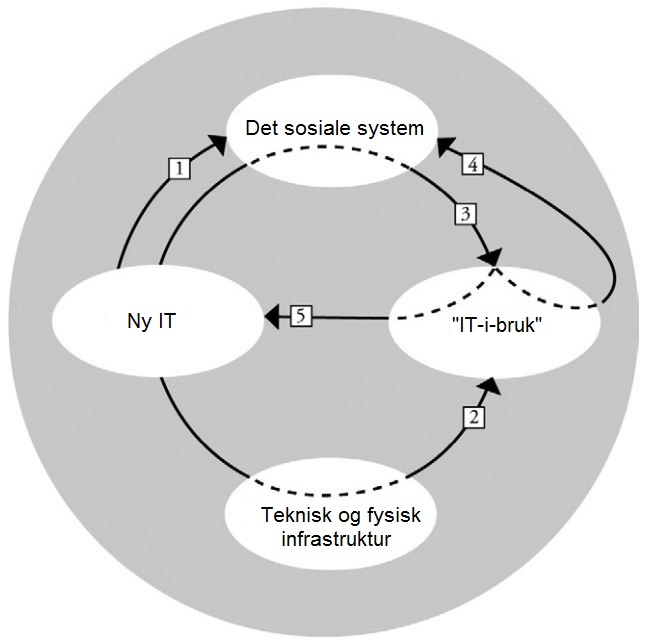
\includegraphics[scale=0.4]{ISTA.jpg}
\caption{ISTA \citep{Harrison}, oversatt av forskerne}
\label{fig:ISTA}
\end{figure}

\noindent
ISTA er basert på fem ulike interaksjoner mellom komponentene i et sosioteknisk system:  

\begin{enumerate}
\item Den første typen interaksjon viser hvordan ny IT endrer det eksisterende sosiale systemet, deriblant arbeidsmønstre, kommunikasjon og relasjon mellom helsepersonell. Teknologien kan eksempelvis føre til at helsepersonell må bruke mer tid på dokumentasjon enn tidligere, eller redusere den direkte kommunikasjonen ansikt-til-ansikt.
\item Dersom ny IT ikke er tilpasset eksisterende teknisk og fysisk infrastruktur, kan det oppstå utilsiktede konsekvenser, eksempelvis forsinkelse, tap av data og feil. Manglende tilpasning av IT til den fysiske settingen hvor den skal tas i bruk kan medføre bruk og workarounds som har negative effekter på sikkerhet, kvalitet og effektivitet. Teknologien kan eksempelvis være plassert slik at den er problematisk å aksessere eller flytte, eller befinne seg i omgivelser preget av støy go med mange mennesker tilstede. Plassering av arbeidsstasjoner trekkes frem som et poeng, da upassende plassering av denne kan redusere den direkte kommunikasjonen, og øke antall distraksjoner. 
\item Fortolkninger og tilpasninger av ny IT vil ofte føre til praksiser som skiller seg fra tenkt bruk. Denne bruken oppstår fordi det opprinnelige designet ikke reflekterer de eksisterende arbeidsmønstre og sosiale relasjoner, og workarounds oppstår som resultat av dette.
\item Den fjerde interaksjonen illustrerer at implementering av ny IT er en rekursiv prosess. Det sosiale systemet påvirker hvordan teknologien brukes, samtidig som denne bruken påvirker det sosiale systemet. Et eksempel på dette kan være at ansatte ikke bruker teknologien slik deres ledere ønsker. Hvis slik bruk vedvarer og tillates, kan det dermed oppstå en endring i maktforholdet mellom ledere og ansatte.  
\item Som et resultat av at brukere gjør lokale tilpasninger som skiller seg fra tenkt bruk, kan utviklere og ledere være tvunget til å gjøre endringer i teknologien.
\end{enumerate}



\section{FITT-rammeverket}
\label{sec:fitt-remmeverket}

FITT (Fit between Individuals, Task and Technology)-rammeverket er et system for å lettere kunne analysere og identifisere de sosiotekniske faktorene som påvirker innføring av nye IT-applikasjoner og -systemer i helseomsorgen, og dermed kunne peke på hvilke faktorer det er som hinderer en optimal utnyttelse av systemet. Rammeverket er bekrevet i sin helhet i \citep{FITT}.

\noindent
Rammeverket deler settingen IT-systemet skal brukes i inn i tre objekter (se figur \ref{FITT-arkitekturen}); (1) $"$Individ$"$, det vil si enkeltbrukere eller brukergrupper av systemet og de som utfører alle oppgaver på arbeidsplassen. (2) $"$Oppgave$"$, er helheten av oppgaver og arbeidsprosesser som må utføres av brukeren med den gitte teknologien. (3) $"$Teknologi$"$, som er det tekniske systemet (program- og maskinvare og nettverk) og andre verktøy som individene bruker for å utføre oppgavene, inkludert papir-verktøy.
$"$Organisasjon$"$ blir ikke behandlet som et eget objekt i denne sammenhengen, men kan sees som en del av enten bruker-objektet (i betydningen at brukerene jobber i forskjellige roller og grupper i en organisasjon) eller oppgave-objektet (i betydningen at oppgavene og prosessene er organisert på en gitt måte).

\noindent
De tre objektene har innehar forskjellige egenskaper, som kan være tilstede i større eller mindre grad. For et individ kan egenskaper være IT-kunnskap, motivasjon og interesse for oppgaven som skal utføres, fleksibilitet og åpenhet for endringer i arbeidsmåte, team-kultur, organisatorisk kontekst, sammarbeidet innenfor team og politikk innen en organisasjon. For en oppgave kan det være organisering av oppgavene som skal gjennomføres, gjensidig avhengighet mellom oppgavene og oppgavenes grad av kompleksitet. Teknologien kan ha stabilitet og brukbarhet ved et program- eller maskinvare-verktøy, verktøyets kostnad, funksjonalitet, tilgjengelig teknisk infrastruktur, integrasjon av verktøy og verktøy tilgjengelig i en gitt klinisk situasjon. Dette er ikke fullstendige lister av egenskaper, men kan likevel gi en forståelse for hva slags egenskaper det kan være snakke om.

\begin{figure}[H]
\centering
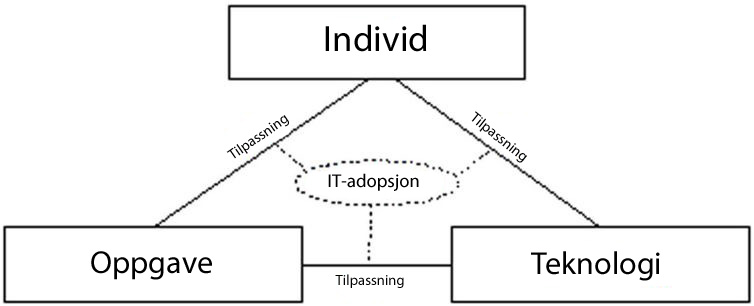
\includegraphics[scale=0.4]{FITT_norsk.jpg}
\caption{FITT-arkitekturen (fritt oversatt av forfatterene. Orginalen kan sees i \citep{FITT})}
\label{FITT-arkitekturen}
\end{figure}

\noindent
Videre ser rammeverket på hvordan disse objektene med sine egnskaper passer (fit) sammen, og sammspillet mellom dem. Fokuset for rammeverket er nettopp dette \emph{samspillet mellom} objektene (og deres egenskaper), og ikke objektene i seg selv. Med denne tilnærmingen kan vi nå definere målet med IT-ledelse som de å finne en optimal tilpassning (fit) mellom bruker, oppgave og teknologi. Dersom objektene mangler, eller har lite utviklede egenskaper som er nødvendig for et optimalt samspill med ett av de andre objektene kan man direkte påvirke egenskapene til det enkelte objektet. Et eksempel ved ingen eller dårlig IT-kunnskap hos brukerene (individ) kan være å gi de ansatte opplæring som øker tilstedeværelsen av denne egenskapen. Siden dette er tiltak som påvirker objektene direkte, vil vi kunne si at det er en indirekte påvirkning på samspillet mellom objektene.

\noindent
Det vil selvfølgelig alltid finnes eksterne faktorer som er vanskeligere eller umulig å påvirke, som høy utskiftning av stab, eller nye lover og regler. Disse eksterne faktorene fører til at det aldri vil oppstå en statisk situasjon med hensyn på de tre dimensjonene av samspill, og derfor heller ikke optimaliseringen av disse.

\noindent
Ved å bruke dette rammeverket kan man lettere se hvor eventuelle problemer ved innføringen av systemet ligger. En vanlig feiltolkning er at problemer som ligger i samspillet mellom brukerene og oppgaven blir tillagt teknologien. Et eksempel på dette er dersom innføringen av et nytt IT-system gir brukerene en større mengde dokumentasjonsoppgaver. Ofte vil det nye systemet (teknologien) få skylden for dette, mens problemet ligger i brukerens misnøye med oppgaven, og ikke har noe med teknologien å gjøre.


\chapter{Metode}
\label{chp:metode} 

Det finnes flere måter å klassifisere og karakterisere ulike former for forskning, men en av de vanligste er å skille mellom \textit{kvalitative} og \textit{kvantitative} forskningsmetoder \citep{Myers13, Tjora}. Kvalitative metoder er velegnet dersom hensikten er å forstå sosiale og kulturelle aspekter ved mennesker og organisasjoner, hvis forskningen er utforskende, eller man ønsker å studere et spesielt emne i dybden \citep{Myers13}. En slik tilnærming vil i større grad avdekke i hvilken \textit{kontekst} en handling eller avgjørelse blir utført, og kan derfor hjelpe forskere å forstå hvorfor informantene handler som de gjør. Med et sosioteknisk utgangspunkt, var det naturlig å benytte forskningsmetoder som genererte kvalitative data i arbeidet med denne studien.

\noindent
Forskerne fikk i sitt arbeid med fordypningsprosjektet, \citep{Sund13}, god kjennskap til hvordan pasientsignalsystemet var \textit{tenkt} brukt. Da denne masteroppgaven var godkjent av NSD\footnote{Norsk samfunnsvitenskapelig datatjeneste \citep{NSD}.} og REK\footnote{Regionale komiteer for medisinsk og helsefaglig forskningsetikk \citep{REK}.}, hadde forskerne større frihet til å gå ut i feltet. For å få en større forståelse av sykepleiernes \textit{reelle} arbeidspraksis, ble det derfor utført observasjoner ved tre ulike avdelinger ved St. Olavs Hospital. I løpet av denne observasjonsperioden ble det avdekket tydelige variasjoner i arbeidspraksis, og forskningsområdet ble dermed avgrenset til å omhandle disse. Det ble deretter utført nye observasjoner med spisset fokus. På bakgrunn av erfaringene gjort under observasjonsperioden ble det utarbeidet intervjuguider, og avslutningsvis ble det gjennomført intervjuer med seksjonsledere og pleiere fra de observerte avdelingene. Dette utgjorde en triangulering av forskningsmetoder, som styrket resultatenes kvalitet.

\noindent
I dette kapittelet vil valg av forskningsmetoder bli belyst. Resultatene av disse vil bli presentert i kapittel \ref{chp:resultater}, og deretter diskutert i kapittel \ref{chp:diskusjon}. 

\section{Hensikt og forskningsspørsmål}
Med bakgrunn i forskernes prosjektoppgave \citep{Sund13}, var utgangspunktet for dette arbeidet å videre undersøke hvordan systemet kan endres for å bedre møte sykepleiernes behov. Det ble derimot tidlig avdekket tydelige ulikheter i sykepleiernes anvendelse av systemet, og forskerne valgte å vinkle forskningsspørsmålene annerledes. Motivasjonen for forskningsarbeidet ble dermed å kartlegge sykepleiernes anvendelse av pasientsignalsystemet, og å identifisere ulikheter i bruk. Videre ønsket forskerne å svare på hva som kan være årsaker til disse forskjellene. Dette resulterte i to forskningsspørsmål:

\begin{enumerate}
\item Hvordan brukes pasientsignalsystemet ved St.Olavs Hospital forskjellig i, og mellom ulike avdelinger? 
\item Hvilke faktorer kan være årsak til disse forskjellene?
\end{enumerate}

\noindent
For å besvare disse spørsmålene gjennomførte forskerne observasjoner og intervjuer ved tre avdelinger ved St.Olavs Hospital. Dataene fra innsamlingen ble deretter analysert, og relevant teori ble valgt i tråd med stegvis-deduktiv induktiv metode. Forskningsmetodene som ble anvendt belyses videre i dette kapittelet.
\section{Etnografi}
\label{section:etnografi} 

Etnografi er en kvalitativ metodikk som innebærer å studere en gruppe mennesker i en gitt setting, og er en hensiktsmessig tilnærming for å forstå handlinger og oppfatninger fra informantenes perspektiv \citep{Blomberg93, Reeves08, Nardi97}. Som en mulig følge av fremveksten av CSCW på 1980-tallet, oppsto samtidig en større interesse for å utforske anvendelsen av etnografiske metoder for å forstå gruppers arbeidsaktiviteter, og metodene har blitt stadig mer populære innen HCI-feltet \citep{Blomberg93, Millen00}. Tradisjonell etnografisk forskning innebærer ofte et bredt forskningsområde, hvor feltarbeidet utføres over en lengre tidsperiode. I prosjekter med begrenset tid for gjennomføring, vil det derimot være nyttig å anvende feltmetoder som kjennetegner \textit{hurtig etnografi} \citep{Millen00}. Dette innebærer å avgrense forskningsområdet, identifisere nøkkelinformanter, bruke interaktive observasjonsteknikker og å utføre en kollektiv analyse av datamaterialet. Da arbeidet i dette prosjektet var begrenset av både tid og tilgang til feltet, ble alle disse elementene inkludert i utførelsen av feltarbeidet.




\section{Observasjon}
\label{section:observasjon} 

 Observasjon kan være en effektiv og god måte å finne ut hva mennesker gjør i praksis, fremfor hva de sier de gjør, eller burde gjort \citep{Oates}.



 Som beskrevet av \citep{Millen00} kan en slik etnografisk metode få frem brukerkrav som brukerne selv ikke uttrykker, og den gir forskerne en rikere forståelse av brukskontekst og arbeidsomgivelser. \citet{Blomberg93} diskuterer relasjonen mellom etnografi og design, hvor etnografen vektlegger å forstå menneskers oppførsel og aktiviteter, mens designerens fokus er å designe artefakter til støtte for disse aktivitetene. Designeren bruker dermed mer tid på å teste og evaluere sine løsninger med hensyn til brukernes behov og evner, og mindre tid på å faktisk forstå den støttede oppførselen \citep{Blomberg93}. I tilknytning til fremveksten av CSCW, har et større fokus blitt rettet mot å anvende etnografiske metoder for å forstå gruppearbeid og å bruke denne kunnskapen ved design.

\subsection{Rolle}
- deltagende observasjon
- åpen observasjon

- varierte mellom deltagende observatør og fullstendig observatør =>interaktiv observatør(Tjora)

\subsection{Utførelse}

\subsection{Utfordringer}

\subsection{Intervju}
\label{sec:intervju}

Intervju er den mest utbredte datagenereringsmetoden innen kvalitativ forskning, med den hensikt å studere informantenes \textit{subjektive} meninger, holdninger og erfaringer. Innen SDI-modellen har intervjuet som mål å generere refleksjon blant deltagerne \citep{Tjora}.  


Strukturerte intervjuer minner om muntlige spørreundersøkelser, hvor intervjueren spør forhåndsbestemte, identiske spørsmål ved hvert intervju. Semi-strukturerte intervjuer tillater  derimot større frihet, eksempelvis ved at spørsmål legges til, eller stilles i en annen rekkefølge enn tenkt. 



\subsubsection{Intervjuguide}
Observasjonsperioden avdekket tydelige forskjeller i sykepleiernes arbeidspraksis, både internt og mellom de ulike avdelingene. Intervjuenes hensikt var dermed å avdekke faktorer som kunne forklare disse forskjellene fra informantenes perspektiv. 

\subsubsection{Intervjuobjekter og utførelse}



Det ble gjennomført semi-strukturerte intervjuer med seksjonsledere og pleiere fra hver observerte avdeling, se tabell \ref{detaljerintervju} for detaljer. Det ble utarbeidet to intervjuguider, en for seksjonsledere og en for pleiere, se tillegg \ref{chp:appendix_intervjuguide_seksjonsledere} og \ref{chp:appendix_intervjuguide_pleiere}.



 På forhånd ble intervjuenes tidsramme estimert til 30 minutter, men intervjuenes lengde ble tilpasset hver informant, avhengig av hvor mye de ønsket å fortelle. Intervjuenes varighet varierte mellom 15-20 minutter for pleierne, og 30-40 for seksjonslederne. 


\begin{table}[H]\centering
    \begin{tabular}{ |l|l|l|l|l|l| }
    \hline
    Intervju & Avdeling & Intervjuobjekt \\ \hline
       I1 & A2 & Seksjonsleder \\ \hline
       I2 & A2 & Sykepleier \\ \hline
       I3 & A2 & Sykepleier \\ \hline
       I4 & A1 & Assisterende seksjonsleder \\ \hline
       I5 & A1 & Hjelpepleier \\ \hline
       I6 & A3 & Seksjonsleder \\ \hline
       I7 & A3 & Sykepleier \\ \hline
       I8 & A3 & Sykepleier \\ \hline
    \end{tabular}
    \caption {Detaljer for intervjuer}
    \label{detaljerintervju}
\end{table}
 






- rolle
- tid og sted
- lydopptak

\section{Dokumentstudie}
\label{sec:dokumentstudie}
Ifølge \citet{Tjora} er dokumentene som brukes i et dokumentstudie i utgangspunktet skrevet for andre formål enn forskning. Slike dokumenter fungerer gjerne som bakgrunns- eller tilleggsdata, og kan være casespesifikke eller generelle. Dokumentene kan være eneste kilde til empiri eller kun fungere som tilleggsdata. 

\noindent
Dokumenter har i dette forskningsarbeidet blitt brukt både som bakgrunns- og tilleggsdata. Eksempler på førstnevnte har vært offentlige dokumenter som omhandler utbyggingen av det nye sykehuset, eksempelvis utforming av fysisk arkitektur \citep{Aslaksen, Sintef-sengetun} og teknisk infrastruktur \citep{TU}, noe som ga forskerne en dypere forståelse av utbyggingens omfang. Dokumenter som er brukt som tilleggsdata omfatter brukerveiledninger til pasientsignalsystemet, samt strategidokumenter og informasjon hentet fra St. Olavs Hospitals hjemmesider \citep{BrukermanualforPasientsignalogPasientsignalapplikasjon, BrukerveiledningforPasientsignal, BrukerveiledningforTradlostelefon, styring13, stolavs}. 

\noindent
Opplæringsmaterialet ble studert for å få en tydelig forståelse av hvordan systemet er tenkt brukt, samtidig som det var av relevans for forskningsområdet å identifisere hvilket opplæringmateriell som er tilgjengelig for sykepleierne.
\section{Stegvis-deduktiv induktiv metode}
\label{section:sdi} 
Analyse av kvalitative data betegner en prosess hvor forskerne forsøker å forstå de empiriske dataene som er samlet inn. Analysen av datamaterialet er blitt utført etter en SDI-metodisk tilnærming (se figur \ref{SDI}). \citet{Tjora} beskriver denne som \textit{$"$en skjematisk modell for kvalitativ forskning, hvor grunnprinsippet er en induktiv utvikling fra empiri til konsepter eller teorier, med deduktive trinnvise tilbakekoblinger. Målet er konseptutvikling og kvalitetssikring.$"$} De oppadgående pilene viser den induktive prosessen hvor forskningen er empiridrevet, mens de nedadgående pilene viser det deduktive arbeidet hvor forskningen i større grad er teoridrevet.

\begin{figure}[H]
\centering
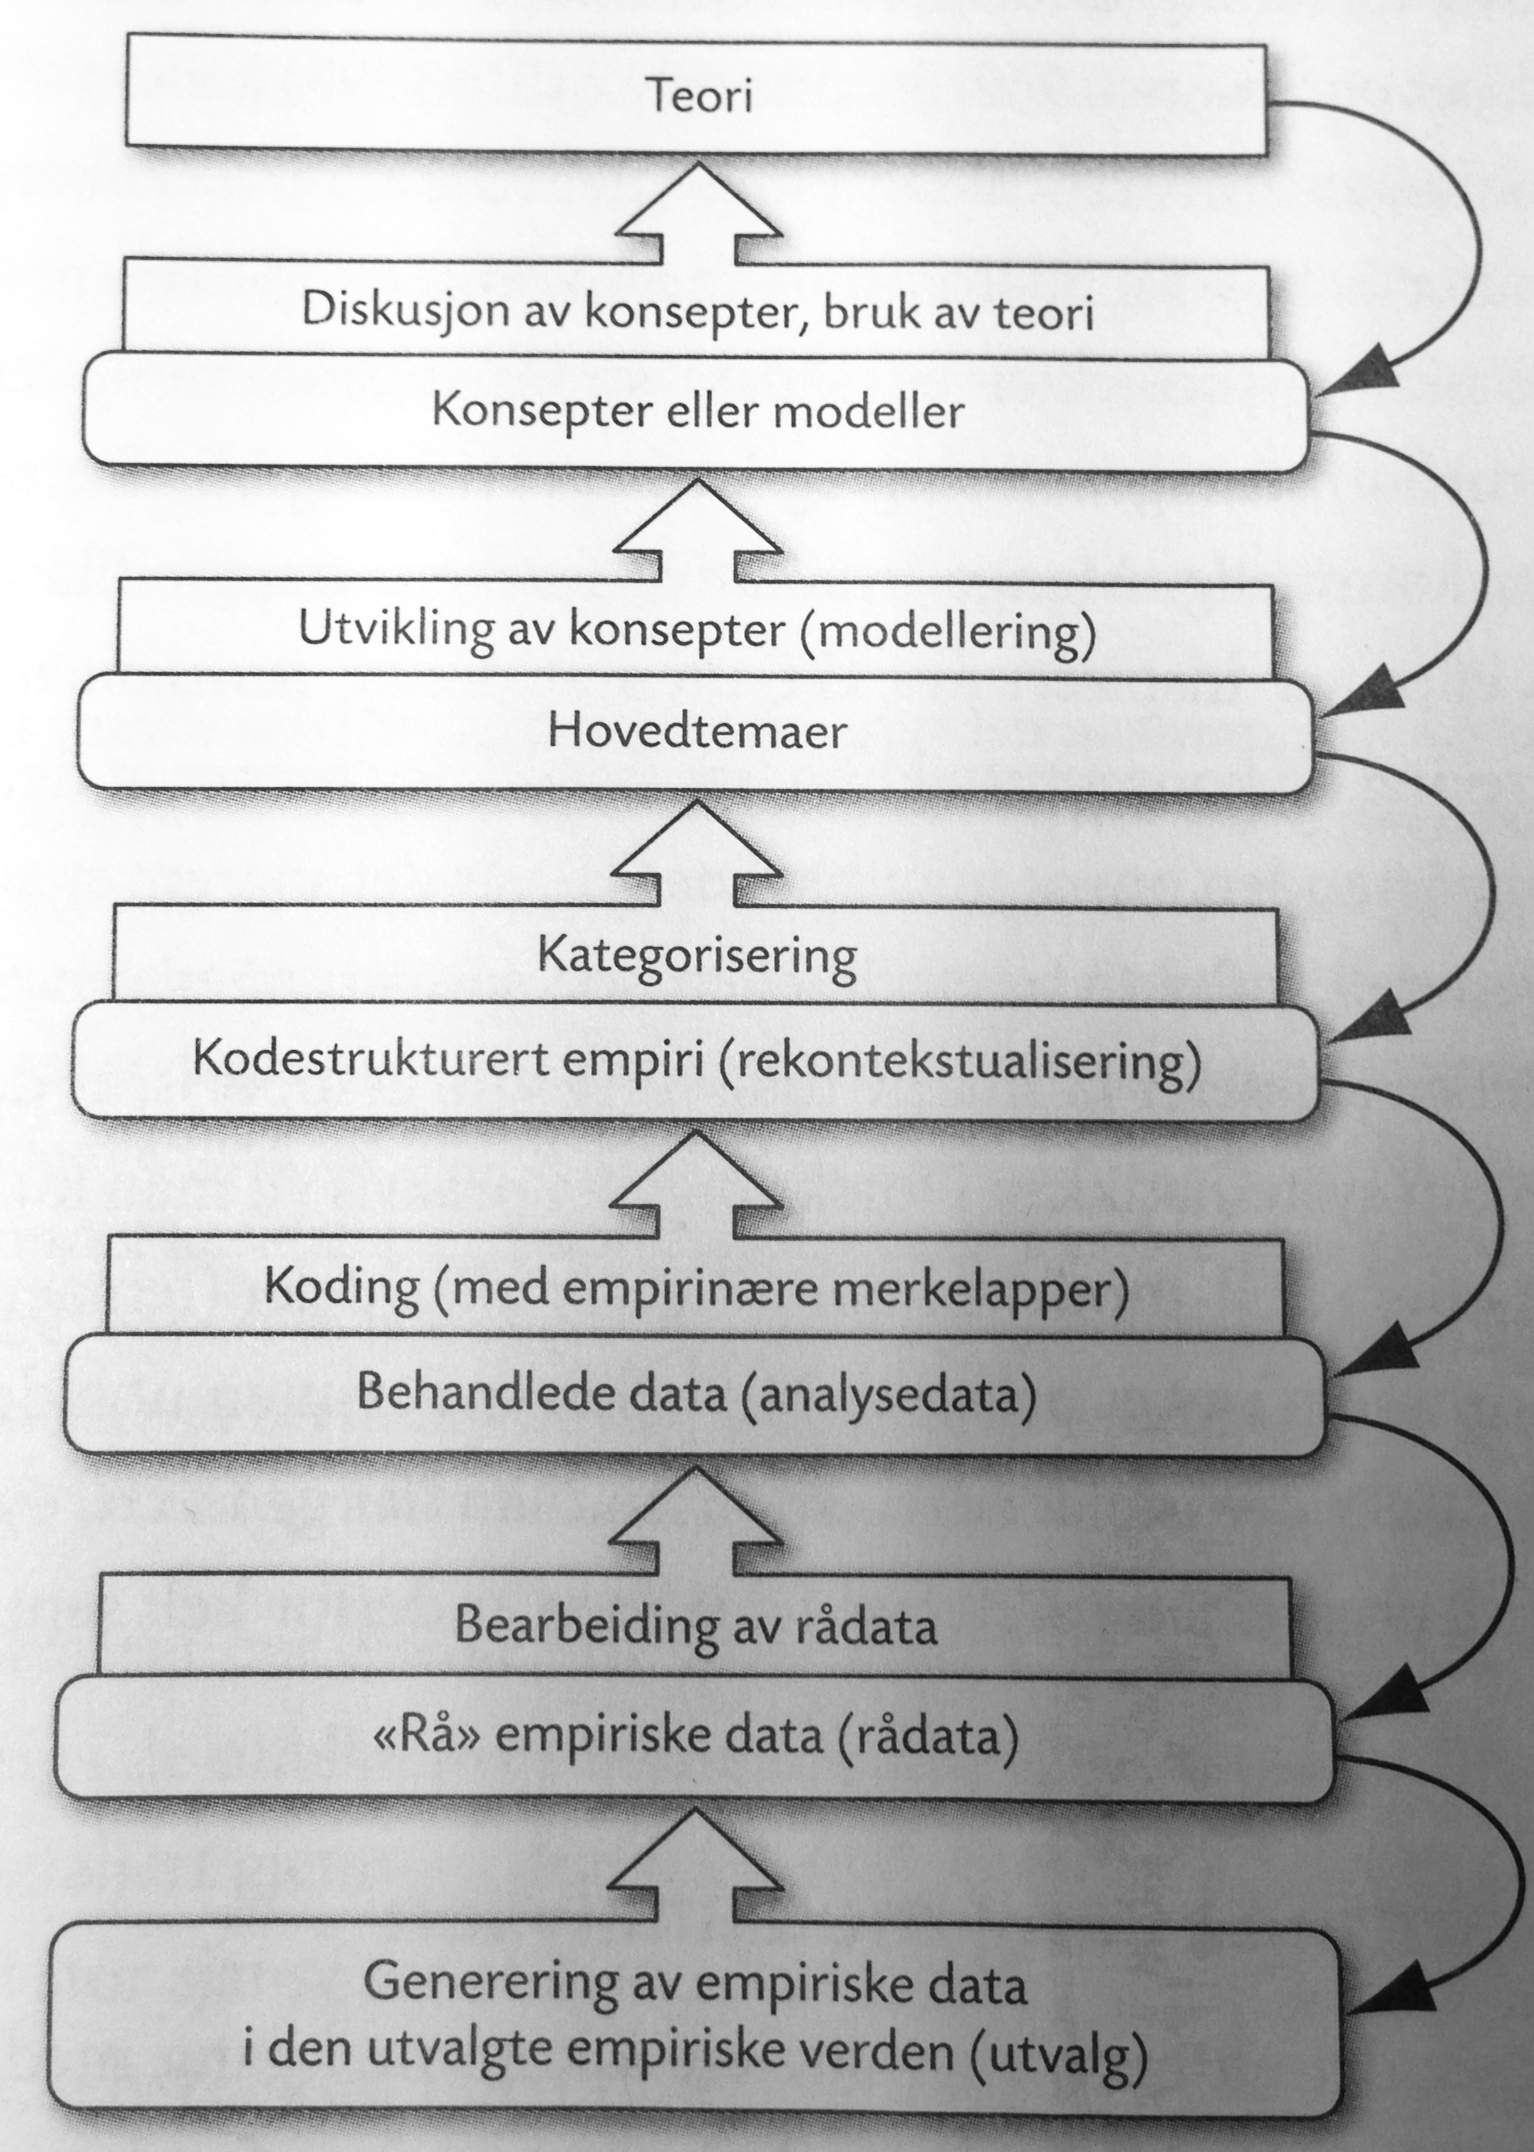
\includegraphics[scale=1]{SDI.jpg}
\caption{Stegvis-deduktiv induktiv metode \citep{Tjora})}
\label{SDI}
\end{figure}

\noindent
Feltnotatene fra første observasjonsperiode ble transkribert, og deretter kodet og kategorisert ved bruk av dataprogrammet RStudio \citep{Rstudio}. Kodingen av observasjonsdataene resulterte i nærmere 100 koder, og forskerne jobbet på denne måten induktivt med materialet. Det høye antallet koder forklares ved at forskerne genererte detaljerte, tekstnære koder fra en stor mengde data \citep{Tjora}. For å kunne luke ut empiri som ikke var relevant for videre forskning ble kodene kategorisert i 11 kategorier. Dette ga en strukturert oversikt over forskningsområdet og forskerne formulerte forskningsspørsmål som det videre arbeidet søkte svar på. Arbeidet beveget seg dermed fra konseptutviklingsfasen til en ny runde med generering av empiriske data. Feltnotatene fra andre observasjonsperiode ble kodet og kategorisert med nærmere 50 koder og 5 kategorier. Etter observasjonsperioden utpekte det seg dermed sentrale temaer som videre formet intervjuguidene. Lydopptakene fra intervjuene ble transkribert og brukt som støtte til observasjonsdataene for å utdype, sammenligne og avdekke forskjeller mellom forskernes og informantenes oppfatninger. Avslutningsvis forsøkte forskerne å konseptualisere avdekkede funn ved å diskutere disse i lys av relevant teori. 



\chapter{Resultater}
\label{chp:resultater} 
Forskerne vil i dette kapittelet redegjøre for funn gjort under observasjoner og intervjuer. På tross av at funnene er komplekse og i stor grad henger tett sammen, er de her inndelt etter de tre objektene: teknologi, individ og oppgave. Dette er gjort for å lettere identifisere egenskapene ved de enkelte objektene, og i tråd med ISTA- og FITT-rammeverket (se kapittel \ref{sec:fitt-rammeverket}) vil samspillet mellom disse bli diskutert i kapittel \ref{chp:diskusjon}.

\begin{table}[H]\centering
    \begin{tabular}{ |l|l|l|l|l|l| }
    \hline
    Avdeling & Intervjuobjekt & Referanse \\ \hline
       A1 & Assisterende seksjonsleder & L-A1 \\ \hline
       A1 & Hjelpepleier & P1-A1 \\ \hline
       A1 & Sykepleier & P2-A1 \\ \hline
       A2 & Seksjonsleder & L-A2 \\ \hline
       A2 & Sykepleier & P1-A2 \\ \hline
       A2 & Sykepleier & P2-A2 \\ \hline
       A3 & Seksjonsleder & L-A3 \\ \hline
       A3 & Sykepleier & P1-A3 \\ \hline
       A3 & Sykepleier & P2-A3 \\ \hline
       - & IKT-rådgiver ved St. Olavs Hospital &  \\ \hline
    \end{tabular}
    \caption {Referanser for intervjuobjekter}
    \label{referanserintervju}
\end{table}

\begin{table}[H]\centering
    \begin{tabular}{ |l|l|l| }
    \hline
    Observasjon & Avdeling & Referanse \\ \hline
    O1          & A1       & O1-A1     \\ \hline
    O2          & A2       & O2-A2     \\ \hline
    03          & A1       & O3-A1     \\ \hline
    O4          & A2       & O4-A2     \\ \hline
    O5          & A2       & 05-A2     \\ \hline
    O6          & A2       & O6-A2     \\ \hline
    O7          & A1       & O7-A1     \\ \hline
    O8          & A3       & O8-A3     \\ \hline
    O9          & A1       & 09-A1     \\ \hline
    O10         & A3       & O10-A3    \\ \hline
    O11         & A3       & O11-A3    \\ \hline
    O12         & A3       & O12-A3    \\ \hline
    O13         & A3       & O13-A3    \\ \hline
    O14         & A3       & O14-A3    \\ \hline
    O15         & A1       & O15-A1    \\ \hline
    O16         & A1       & O16-A1    \\ \hline
    O17         & A2       & O17-A2    \\ \hline
    O18         & A2       & O18-A2    \\ \hline
    \end{tabular}
    \caption {Referanser for observasjoner}
    \label{referanserobservasjon}
\end{table}

\section{Teknologi}
Teknologi beskrives av FITT-rammeverket som det tekniske systemet og de verktøy som brukes for å utføre oppgaver. Egenskaper ved teknologien kan blant annet være dens stabilitet, brukbarhet, infrastruktur og funksjonalitet. 

\subsubsection{Teknisk utforming}
Avdelingene har ulik teknisk utforming og det er derfor forskjeller på hvilke pasientsignaler som varsles hvor, og på hvilke enheter. Sløyfene knytter sengetunene sammen, og avgrenser hvor pasientsignaler og hasteanrop varsles gjennom det faste systemet. IKT-rådgiver ved sykehuset fortalte at disse sløyfene i utgangspunktet var små, men etter sykepleiernes ønske ble de gjort større. Dette fordi sykepleierne også ønsket å motta signaler fra tun utenfor den opprinnelige sløyfen. I ettertid har det derimot vært en utfordring at pleierne ønsker å gjøre disse sløyfene mindre, for å minke antall varslinger. Å endre på disse sløyfene er ifølge IKT-rådgiver ressurskrevende, og man ønsker derfor å la disse være som de er, og heller endre logikken i det trådløse systemet. Eksempelvis ved at pleierne logger seg på som disponible på tun utenfor egen sløyfe, slik at de mottar varslinger på telefon.

\noindent
Veggpanelene på avdeling A1 viser signaler fra alle tun, da hele avdelingen ligger på samme sløyfe. Ved avdeling A2 ligger det ene sengetunet på en annen sløyfe enn de to andre, og pasientsignaler fra det ene sengetunet varsles dermed ikke på veggpanelene til de to andre, og motsatt. Dette medfører at pleierne er avhengige av å bruke telefonene for å motta pasientsignaler på tvers av disse sløyfene, noe som er spesielt viktig på kvelds- og nattskift hvor det er færre pleiere på jobb. For avdeling A3 gjelder det samme, da de fire sengetunene er fordelt på to etasjer, hvor de to tunene i hver etasje ligger på samme sløyfe.

\subsubsection{Telefonsamtaler}
IP-telefonen som benyttes som en del av pasientsignalsystemet har vært et sentralt aspekt ved forskningsarbeidet, og det ble avdekket tydelige ulikheter i bruk av denne. På alle tre avdelinger går sykepleierne med hver sin telefon, og bruker den for å ringe, og motta telefonanrop, men bare avdeling A2 og A3 bruker den for å motta pasientsignaler. Både seksjonsledere og pleiere ga under intervjuene uttrykk for at telefonen ofte brukes i situasjoner hvor de ønsker å komme i direkte kontakt med andre pleiere. L-A1 og P1-A1 påpeker at de bruker mindre tid på å lete etter hverandre nå som de går med telefon.   

\noindent
Generelt uttrykker flere at telefonen er et nyttig verktøy for kommunikasjon med andre, og at det er dette de bruker den mest til. Det trekkes derimot frem som et sentralt problem på alle avdelinger at pasientsignaler varsles i telefonsamtaler, da varslingen oppleves som svært forstyrrende, spesielt blant seksjonslederne og pleiere i roller hvor de ringer mye. P2-A2 forklarte det slik: \textit{ $"$... hvis jeg snakker i telefonen, [...] og så ringer [et pasientsignal], så bryter den gjennom, og det er forferdelig å snakke i telefonen$"$}. L-A2 understreker at det i hans tilfelle vil være uaktuelt å motta pasientsignaler på sin telefon, da han har mange telefonsamtaler i løpet av en dag. P1-A3 forklarte at de løser dette problemet med å heller bruke fasttelefonen på tunet, mens L-A2 fortalte at ansvarshavende sykepleier ofte går med to telefoner, hvor den ene mottar pasientsignaler og den andre telefonsamtaler. I samtale med IKT-rådgiver ved sykehuset ble forskerne gjort oppmerksomme på at systemet vil bli endret, slik at signaler ikke lenger varsles under telefonsamtaler, men heller sendes direkte videre til neste mottaker.

\subsubsection{Avbrytelser og støy}
Ved innflytting i nye lokaler forsøkte avdeling A1 å bruke telefonen slik den er tenkt, til mottak av pasientsignaler, men etter en prøveperiode på to uker konkluderte de med at de ikke ønsket å benytte denne løsningen. Dette til tross for at de er pålagt slik bruk. Seksjonsleder og pleiere viste til flere årsaker for dette. Pleierne står ofte i stell, og har av hygieniske årsaker ikke alltid mulighet til å besvare signalene som mottas. L-A1 påpekte videre at de har en pasientgruppe som hyppig utløser pasientsignaler. Dette resulterte i mye støy beskrevet av L-A1 som \textit{$"$uutholdbar$"$}. Forskerne kan imidlertid ikke si å ha observert at pasientgruppen på avdeling A1 utløser flere signaler enn pasientene på de to andre avdelingene. Forskerne så heller ikke en sammenheng mellom mengden utløste signal, tid og avdeling. 

\noindent
Avdeling A1 opplevde også at pasienter ble forstyrret av støyen, og en av sykepleierne fortalte under observasjonene at noen pasienter mistet tillit til pleierne da det ringte i lommen deres uten at de besvarte anropet. Ved de to andre avdelingene brukes telefonen i større grad slik den er tenkt, men også der trekkes støy frem som en vesentlig utfordring. P2-A2 beskrev opplevelsen av varslinger på telefon slik: \textit{ $"$...det med telefon og sånn, det synes jeg [er] veldig urolig, urolig hverdag, bråkete. Særlig hvis du står i stressende, pressende situasjoner så ringer det, og ringer, og ringer, og ringer...$"$}. 

\noindent
Hun fortalte videre at pasienter vegrer seg for be om assistanse hvis de tror sykepleierne har mye å gjøre:

\noindent
\textit{$"$... [pasientene sier] «oi, vi hører dere har det travelt». Men det trenger ikke være tilfellet. Så ringer dem ikke på. [...] Men vi trenger ikke ha det travelt selv om det ringer, for det kan jo ringe fra de andre tunene. Jeg får jo inn det på min telefon også. Det kan jo være en der borte som ligger på klokken hele dagen, og det vil jo ikke si at jeg har det travelt.$"$}

\noindent
Til tross for at flere pleiere uttrykte misnøye med lydnivået på telefonene, poengterte de samtidig at det gir nødvendig informasjon, og en indikasjon på hvor mye det er å gjøre på avdelingen. Tidligere kunne lyden på telefonen skrues av, men dette skapte en risiko for at signaler ikke ble oppdaget. Lydnivået kan per i dag derfor ikke skrues lavere enn nivå to. Under observasjon ved avdeling A2 ble forskerne fortalt at noen pleiere valgte å teipe over høyttaleren på telefonen for å dempe lyden. Et annet eksempel ble gitt under intervjuet med P1-A2, som fortalte om en pleier som hadde pakket telefonen inn i bobleplast.

\noindent
Pleiere fra alle tre avdelinger påpekte at støy fra telefonen er et problem om natten i tilfeller hvor sykepleieren er inne hos en pasient når det utløses et signal. P2-A2 ser nytten av å gå med telefonen på nattevakt, da hun ønsker å være tilgjengelig for kolleger og pasienter som trenger hjelp. Samtidig uttrykte hun at det er utfordringer knyttet til dette: \textit{ $"$... så har jeg jo opplevd at pasienter våkner og ikke får sove igjen. Og det er jo en bakdel$"$}. Hun fortalte videre at pleiere på avdelingen derfor iblant legger igjen telefonen utenfor rommet for å unngå dette problemet. For å ikke være fullstendig utilgjengelig velger de fleste likevel å tilstedemarkere seg, da varslingen på rompanelene ikke oppleves som like forstyrrende som den på telefonen. For avdeling A2 og A3 vil det være svært alvorlig å være utilgjengelig på telefon, da disse avdelingene ikke mottar signaler fra alle tun på sengeposten på panelene. Dette gjelder også på dagtid, og er dermed et av de mest fremtredende argumentene for å motta pasientsignaler på telefon. Forskerne observerte imidlertid at pleierne i flere tilfeller ikke tilstedemarkerte seg på rom. Gjennom intervjuene ble det klart at det varierer hvorvidt dette er et bevisst valg, eller en forglemmelse. Pleierne ser derfor fordelen av å motta signaler på telefon, da dette oppleves som en sikkerhet i de tilfeller hvor de glemmer å markere seg. Dette gjelder også i tilfeller hvor de befinner seg på steder uten veggpaneler, eksempelvis på møterom eller utenfor avdelingen.

\subsubsection{Interaksjon med telefon ved utløst pasientsignal}
Både pleiere og seksjonsledere fra avdelingene A1 og A3 trekker frem telefonens grensesnitt som lite brukervennlig, og beskriver den som tungvint å bruke. L-A1 uttrykte seg slik:

\noindent
\textit{ $"$... det jeg reagerer på når det gjelder IP-telefonen, er at man må sende en hel avdeling på kurs i flere timer for å forstå en telefon. [...] Det er ressurskrevende, og for komplisert. [...] [Den har funksjoner] som er veldig tungvinte, og det er veldig lite selvforklarende, veldig lite brukervennlig, og skiller seg vesentlig fra mobiltelefoner...$"$}.

\noindent
Et interessant funn gjort under observasjonene var at pleierne i relativt liten grad interagerer med telefonene, men heller ser på veggpanelene ved utløste pasientsignaler. Under intervjuene ble det avdekket flere årsaker til dette. For det første vil forsinkelsen i det trådløse systemet føre til at signalet varsles tidligere på panelene enn på telefonene. For det andre er panelene plassert slik at det ofte vil være enklere å se på disse enn å ta telefonen opp fra lommen, samtidig som det i andre tilfeller vil være problematisk å håndtere telefonen, eksempelvis av hygieniske årsaker, eller i situasjoner der det kan oppleves som forstyrrende for pasienten. Dette resulterer i at funksjonaliteten for å bekrefte eller avvise signalet ikke brukes, og dermed heller ikke arbeidslisten. Dette fører til unødvendig støy, da signalet varsles i 15 sekunder før det går videre til neste mottaker. Imidlertid er det flere som påpeker at panelene burde vært større, da det kan være vanskelig å lese fra avstand. Ved avdeling A1 er vaktromsapparatet på det ene sengetunet plassert bak en dør som vanligvis står åpen. Både L-A1 og pleiere fra avdeling A1 ønsker seg et panel i taket, slik de hadde før. Dermed kan de enkelt se hvor signalene er utløst fra uten å måtte gå bort til et veggpanel. P1-A1 kunne i tillegg tenke seg ulike varslingslyder for signaler fra de forskjellige tunene, slik at pleierne enkelt hører om signalet er utløst på deres tun.

\subsubsection{Assistansesignal}
Et interessant funn er sykepleiernes holdning til å utløse hasteanrop. Ifølge sykehusets opplæringsmateriell skal hasteanrop utløses ved behov for assistanse. Observasjonene avdekket derimot for det første at sykepleierne kaller dette signalet for en $"$stansalarm$"$, og for det andre at de helst utløser denne kun i nødsituasjoner. Ved utløst stansalarm forklarte pleierne at alle slipper det de har i hendene og løper for å besvare signalet. I løpet av alle observasjonene ble det kun utløst et hasteanrop, og forskerne så at pleieren ved det observerte tunet løp til det andre tunet. Forskerne observerte også at pleierne i noen tilfeller heller kom ut fra pasientrom for å spørre om hjelp enn å utløse et hasteanrop. 

\noindent
En tydelig forskjell mellom avdelingene er at avdeling A1, som eneste avdeling, kan utløse assistansesignal. Forskerne observerte at dette er en funksjon de bruker mye og er svært fornøyd med, noe pleierne også bekreftet under intervjuene. Denne funksjonaliteten eksisterte ved det gamle sykehuset, men ble ikke videreført i det nye. Avdelingen fikk likevel gjeninnført denne funksjonaliteten da de flyttet inn i nye lokaler høsten 2013, og pleierne beskriver den som noe de \textit{$"$kjempet$"$} for, og \textit{$"$forlangte$"$} å få. Under observasjonene fortalte også en av pleierne fra avdeling A2 at hun savnet assistanseknappen. 

\subsubsection{Feil og forsinkelse}
Pleierne fra avdelingene A2 og A3 opplever at pasientsignalsystemet fungerer slik det er i dag, men påpeker tekniske feil og mangler. De opplever blant annet det de kaller \textit{$"$spøkelsesalarmer$"$}, signaler som ingen har utløst, eller som er utløst fra rom de ikke kjenner til. L-A3 påpeker at dette kan føre til at pleierne blir \textit{$"$immune$"$} mot varslingene på telefonen, noe som også ble bekreftet av P2-A3:

\noindent
\textit{$"$... det er jo litt feilmeldinger og sånn på det da. [...] Det er jo ikke noe særlig. Det blir sånn ulv ulv nesten... $"$}

\noindent 
Forsinkelsen fra det faste til det trådløse systemet fører til at varslingen på telefonen fortsetter etter at en pleier har tilstedemarkert seg på et pasientrom, noe som skaper irritasjon blant pleierne. P1-A3 beskrev det slik: \textit{$"$...så fortsetter den her å pipe i inntil 1-1,5 minutt etterpå, og det er jo enormt irriterende. At når du allerede har utført jobben, så får du fortsatt beskjed om at jobben ikke er påstartet.$"$} Dette ble også observert av forskerne, og forsinkelsen førte i noen tilfeller til at pleiere kom for å besvare signalet selv etter at dette var gjort. 

\section{Individ}
Et individ beskrives av FITT-rammeverket som enkeltbrukere eller brukergrupper av systemet, og er de som utfører alle oppgaver på arbeidsplassen. Egenskaper ved individet kan være IT-kunnskap, motivasjon, åpenhet for endring i arbeidsmåte og teamkultur.

\subsubsection{Holdninger til systemet}
Observasjonene og intervjuene avdekket et bredt spekter av holdninger til systemet. På avdelingene A2 og A3 brukes pasientsignalsystemet i stor grad slik det er tenkt, og seksjonslederne og pleierne opplever at det er et nyttig verktøy. Avdeling A1 har derimot opplevd større motstand mot systemet, og anvender kun deler av det.

\noindent
I overgangen fra det gamle til det nye sykehuset forsøkte avdeling A1 på lik linje med andre avdelinger å benytte telefonen slik den er tenkt. Det ble derimot tidlig et problem at telefonene skapte mye støy og var lite brukervennlige, noe som skapte stor frustrasjon. P1-A1 fortalte under intervjuet at de ikke var forberedt på at flyttingen skulle medføre så store endringer i systemet. Han opplevde at de hadde et velfungerende system, og antok at dette ville bli videreført. Med innføringen av IP-telefoner, samt bortfall av assistanseknappen og panelet i taket, oppsto det derimot negative holdninger til det nye pasientsignalsystemet. Da avdelingen igjen flyttet inn i nye lokaler hadde de en prøveperiode på 14 dager, hvor de på nytt forsøkte å bruke systemet som tenkt. De fikk samtidig tilbake assistanseknappen de lenge hadde ønsket seg. P2-A1 fortalte at pleierne i denne perioden gjorde et forsøk på å få systemet til å fungere, men sa samtidig at de visste at det var en prøveperiode, og at de ikke brukte det optimalt da de ofte ikke godtok signalet på telefonen, men lot det gå videre til neste mottaker. Etter prøveperioden gikk avdelingen tilbake til å ikke motta pasientsignaler på telefon. Både L-A1 og pleierne på avdelingen uttrykte tydelig at de ikke ser nytten av slik bruk. De argumenterer med at de like gjerne kan se på panelene, og at de ofte står i situasjoner hvor de ikke har mulighet til å håndtere telefonen. L-A1 forklarte det slik: 

\noindent
\textit{$"$... en ting er problemene med systemet, det kan man alltids finne løsninger på. Men når det i tillegg ikke er gevinst med noe, da er det vanskelig å få gjennom noe som i utgangspunktet er et problem, det er et system med bare ulemper og ingen fordeler. Det er veldig vanskelig å få gjennom en sånn ting. Hvis vi hadde hatt fordeler med det, så kan vi leve med ulempene. Men å få gjennom noe med bare ulemper, det er vanskelig.$"$}

\noindent
Forskerne avdekket videre at endringer i lyd ikke vil endre avdelingens innstilling til å motta pasientsignaler på telefon. Dette ble tydelig understreket av P2-A1 som sa:

\noindent
\textit{$"$... jeg forstår ikke hvorfor vi skal ha det på telefonen. [...] Hvorfor du skal ned i en lomme for å se hvorfor det ringer liksom. Da må vi jo ha tilgjengelige skjermer, tilgjengelig i tak som sagt, tilgjengelig panel.$"$}

\noindent
P1-A1 ønsker å ha fullt fokus på pasientene, og beskrev sitt forhold til å gå med telefon på seg slik:

\noindent
\textit{$"$... altså når jeg går inn på et pasientrom så er det pasienten jeg har i fokus. Og da er det kun pasienten, og det som skjer utenfor det pasientrommet det blåser jeg i, for at det er det andre mennesker som tar seg av.$"$}

\noindent
Selv om de ikke bruker systemet slik det er tenkt fra produsentens side, opplever avdelingen at de har en velfungerende løsning. L-A1 påpekte imidlertid at det ikke er en god situasjon at de ikke bruker det slik de er pålagt.

\noindent
For avdeling A2 og A3 uttrykte pleierne en generelt mer positiv holdning til systemet, til tross for at holdningene varierte også her. Pleier P1-A2 beskriver det som et $"$kjempeverktøy$"$, mens P2-A2 opplever det til tider som stressende å motta pasientsignaler på telefon. P2-A3 så derimot ikke på dette som et problem: 

\noindent
\textit{$"$Det er veldig greit at du kobler deg på rommene som du har, og at det ringer først til deg. Og at jeg kan avvise det. Det synes jeg er greit.$"$}

\subsubsection{Ansvarsfordeling}
Som tidligere påpekt påvirker avdelingenes tekniske utforming hvordan sykepleierne bruker, og logger seg på systemet. På alle tre avdelinger fordeler pleierne på hvert sengetun ansvaret for pasientrommene mellom seg. Systemet er tenkt slik at pleierne skal logge seg på som primær på sine rom og som disp på andre, og dermed motta pasientsignaler fra disse på sin telefon. Det ble likevel avdekket avvik fra dette, da noen kun logger seg på som primær, og andre kun setter seg som disp på tunet. På kvelds- og nattskift er det få pleiere på jobb, og det er vanlig at de kun setter seg som disp. For å motta pasientsignaler fra andre tun logger pleierne på A2 seg på som disponible på disse. På A3 gjøres dette kun på nattskift. 

\noindent
Pleierne gjør kontinuerlige vurderinger av hvilke oppgaver de skal utføre når, og hvordan de skal håndtere innkommende pasientsignaler. Til tross for at pleierne både under observasjonene og intervjuene ga uttrykk for at de har et felles ansvar for pasientene, fortalte P2-A2 at rollene primær og disp medfører en utfordring:

\noindent
\textit{$"$... det som jeg ser på som er det negative det er vel på en måte at vi setter oss opp på $"$våre pasienter$"$, så hvis jeg er opptatt med en av mine pasienter og det ringer på på de to andre mine pasienter så blir ikke klokkene tatt. De bare avslutter eller kjører telefonen videre, mange ganger, og det synes jeg er feil.$"$}

\noindent
På alle tre avdelinger er det variasjon i hvor lenge pasientene ligger inne, og dermed hvor godt pleierne kjenner dem. De fleste gir likevel uttrykk for at de normalt har tilstrekkelig kunnskap om pasientenes tilstand til å kunne vurdere signalenes hastegrad. Under observasjonene fortalte flere pleiere at pasientene har ulik terskel for å utløse signaler. Mens noen kun gjør det ved alvorlige hendelser, utløser andre signaler oftere. Forskerne observerte også at sykepleierne iblant gjør avtaler med pasientene om å utløse signal ved spesifikke hendelser, og da vet hva signalet gjelder. Til tross for at sykepleierne ga uttrykk for at de besvarer pasientsignalene raskt uansett pasient, observerte forskerne ved flere tilfeller at signaler ringte opp til flere minutter før de ble besvart. Til tross for at det ikke foreligger kvantitative data på dette, opplevde forskerne en tendens til at signalene varsles lenger på avdeling A1 før de blir besvart.  
  
\noindent
L-A2: \textit{$"$... den kulturen med å ta klokker da, den er veldig forskjellig fra sengepost til sengepost, og jeg tror at der det er mest rolig, der sykepleierne antar at det ikke haster når en pasient ringer, så er det nok en kultur for at man kan la det ringe lenge. Og hvis man lar det ringe lenge blir det veldig mye støy – for alle. Og da tror jeg motivasjonen for å bruke systemet blir ganske lav. Nettopp av den grunn.$"$}

\noindent
Under observasjon O1-A1 delte sykepleierne pasientene i to grupper, A og B. Pleierne avtalte å være to stykker sammen på de rommene de visste at stell av pasientene krever mer. Også under O9-A1 delte pleierne pasientene i gruppe A og B, og de serverte mat til $"$sine$"$ pasienter. Under O16-A1 fortalte en av pleierne at de har ansvar for tre rom hver, og hvis de begge er ledige besvarer den som har ansvar pasientsignalet, ellers deler de på å besvare signalene. Også ved avdeling A2 fordeler sykepleierne primæransvar for pasientene, men pleierne uttrykte noe delte meninger om hvorvidt de besvarer signaler fra andre pasienter. Under observasjon O4-A2 fortalte en av pleierne at de forsøker å ha en policy på at de skal hjelpe hverandre, men at noen kun svarer på signaler fra egne pasienter. Under observasjon O6-A2 sa derimot en av pleierne at $"$alle hjelper alle, vi er et team$"$. De fortalte videre at de forsøker å ha ansvar for pasienter de har hatt ansvar for før, som de kjenner godt. Ved avdeling A3 gir pleierne uttrykk for at de normalt fordeler primæransvar for pasientene, som innebærer oppgaver som blant annet stell, medisinering og matservering. I likhet med de andre avdelingene er det primæransvarlig som hovedsakelig besvarer pasientsignal fra sine pasienter, men pleierne understreker at dersom denne er opptatt besvarer andre pleiere signalet. Forskerne observerte at pleierne i større grad besvarte signaler fra egne pasienter på dagskift, mens dette oftere varierte på kveldsskift hvor de var færre pleiere på jobb. Forskerne så aldri at en pleier forlot et pasientrom for å besvare et annet pasientsignal. 

\subsubsection{Opplæring}
Gjennom intervjuene ble forskerne gjort oppmerksomme på at avdelingene selv står for opplæring av nyansatte. Seksjonslederne og pleierne er åpne om at dette fører til at holdninger og rutiner videreføres, som beskrevet av P1-A2:

\noindent
\textit{$"$... det er sikkert individuelle forskjeller [...] hvor nøye man er, også er det sikkert litt i forhold til opplæring. Er det dårlige vaner på en avdeling, og man har opplæring så blir det kanskje til at man lærer det videre litt ubevisst. Som ny er man jo veldig var på hva slags holdninger og sånn de har de man går med, er man litt sløv og bruker det feil så er det kanskje det man lærer bort også.$"$}

\noindent
Selv om pleierne på avdelingene A2 og A3 stort sett er fornøyde med systemet ble det påpekt utfordringer. P1-A2 fortalte at det kan være en risiko at de manuelt må sette seg som disp for å motta signaler fra andre tun, da det kan være nyansatte som ikke er klar over dette.  

\section{Oppgave}
En oppgave beskrives av FITT-rammeverket som helheten av oppgaver og arbeidsprosesser som må utføres av brukeren med den gitte teknologi. Egenskaper ved oppgaven kan blant annet være organisering av oppgavene, gjensidig avhengighet mellom oppgavene og oppgavens grad av kompleksitet.

\subsubsection{Planlagte og tilfeldige oppgaver}
Felles for alle tre avdelinger er at sykepleierne utfører både planlagte og tilfeldige oppgaver. Medisinering, stell og matservering er eksempler på førstnevnte, og disse skjer normalt til faste tider. Et eksempel på sistnevnte er pasientsignaler, som ofte utløses uten forvarsel.  

\noindent
Flere oppgaver innebærer bruk av systemet. For å motta pasientsignaler på rompanelet, og for å formidle sin tilstedeværelse til kolleger, skal sykepleierne tilstedemarkere seg på pasientrom. I tilfeller hvor en sykepleier går inn til en pasient ved utløst pasientsignal, trykker pleierne alltid på tilstedeknappen, da dette avstiller signalet. Hvis det derimot ikke er utløst et signal ble det under observasjonene avdekket store variasjoner i hvorvidt tilstedeknappen benyttes. Pleierne forklarte at dette gjøres oftere i tilfeller hvor de vet at oppgaven på pasientrommet tar tid, mens de ved kortere besøk heller velger å la døren stå på gløtt. Dette ble bekreftet av P2-A3 under intervjuet: 

\noindent
\textit{$"$... noen er vel litt sløve med å logge seg inn på rom da. Å trykke på grønnlyset og sånt. Kanskje litt flinkere til å gjøre det når vi vet at vi skal stelle og sånt. At vi blir der en stund. Men hvis vi bare skal inn å levere medisiner eller noe sånt så, blir det ikke brukt noe grønnlys.$"$}

\subsubsection{Rutiner}
Pleierne fortalte under intervjuene at de ved starten av hvert skift logger seg på telefonen, og de anser dette som en vane. Det var imidlertid ulike synspunkt på hvorvidt det å logge seg på rom er en rutine. Forskerne observerte ved noen tilfeller at pleiere fra tidligere skift fremdeles var logget på som ansvarlige for pasientrom. Pleierne forklarte at de iblant glemmer å logge seg på rom, spesielt hvis det er mye å gjøre, som beskrevet av P2-A2:

\noindent
\textit{$"$... vi er en ganske hektisk avdeling, [så om morgenen] så kan det jo eksplodere her, og da er det kanskje fåtallet av oss... De fleste har vel logget på telefonen, men vi har jo ikke logget oss på systemet, og da [om det eksploderer og vi er i jobb alle mann] tenker vi ikke over det, før kanskje langt utpå formiddagen, at oi, her er det noe som har gått oss hus forbi, så kan vi se at det er nesten ingen som har logget seg på systemet.$"$}

\noindent
P1-A3 fortalte derimot: $"$... det er noe alle gjør. Det er inne, det er rutine nå. Det er ikke noe problem.$"$ 

\noindent
Under samtlige observasjoner observerte forskerne at pleierne iblant glemte å trykke på rødknappen for å fjerne tilstedemarkeringen når de forlot rommet. Dette medfører at signaler varsles inne på pasientrom uten at det er sykepleiere tilstede.

\noindent
På avdeling A1 har det etter innflytting i nye lokaler vært fokus på at pleierne må tilstedemarkere seg, da de ellers ikke vil bli varslet om utløste pasientsignaler og stansalarmer. Forskerne la imidlertid ikke merke til at dette ble gjort i større grad her enn på de andre avdelingene.  

\section{Oppsummering}

\subsubsection{Teknologi}
\begin{itemize}
\item Ulikheter i teknisk utforming fører til at sykepleierne ved avdeling A2 og A3 må bruke telefonen for å motta pasientsignaler fra alle sengetun på avdelingen.

\item Varsling av pasientsignaler i telefonsamtaler fører til ulike workarounds.

\item På grunn av støy bruker ikke avdeling A1 for mottak av pasientsignaler. Pleiere ved de to andre avdelingene bruker til telefonen til dette selv om støy også er en problematikk ved disse avdelingene. For å redusere støyen oppstår det også her workarounds.

\item Pleierne uttrykker misnøye med telefonens grensesnitt, og de pleierne som mottar pasientsignaler på telefon interagerer med denne i liten grad ved utløst signal.

\item Det varierer hvorvidt pleierne tilstedemarkerer seg på pasientrom.

\item Avdeling A1 kan utløse assistansesignal. 

\item Det som i opplæringsmateriellet omtales som et hasteanrop til bruk ved behov for assistanse, omtales av pleierne som en stansalarm, og utløses kun i nødsituasjoner.

\item Feil og forsinkelse i systemet fører til frustrasjon blant pleierne.

\end{itemize}

\subsubsection{Individ}
\begin{itemize}
\item Pleierne har svært ulike holdninger til pasientsignalsystemet, spesielt i forhold til varslingen på telefon.

\item I hvilke roller pleierne logger seg på i systemet, og hvordan de fordeler oppgave mellom seg varierer mellom avdelingene, og er avhengig av hvilket skift pleierne jobber.

\item Pleierne forsøker i større grad å besvare signaler fra pasienter de har primæransvar for på dagskift.

\item Det er variasjoner i hvilken grad pleierne besvarer signaler fra pasienter de ikke har primæransvar for.

\item Avdelingene har selv ansvar for opplæring av nansatte, og pleierne er åpne om at dette fører til at holdninger og rutiner videreføres.

\end{itemize}

\subsubsection{Oppgave}
\begin{itemize}
\item Sykepleierne utfører både planlagte og tilfeldige oppgaver.

\item Pleierne velger ofte å la døren stå på gløtt fremfor å tilstedemarkere seg ved korte besøk. 

\item Flere pleiere glemmer ofte å fjerne tilstedemarkeringen når de forlater pasientrom.

\item Pleierne kan glemme å logge seg på i bemanningsplanen i starten av hvert skift, spesielt dersom det er travelt på avdelingen.

\end{itemize}

Den tydeligste forskjellen mellom avdelingene er den negative holdningen A1 har til bruk av telefonen for mottak av pasientsignal, som har resultert i at de ikke bruker denne funksjonen. De mest fremtredende årsakene sykepleierne selv trekker frem er støy, pasientenes reaksjoner, lite brukervennlig brukergrensesnitt og problematikken rundt bruk av telefon i sterile settinger. I dag bruker pleierne ved avdeling A1 kun veggpaneler til mottak av pasientsignaler, men da disse er små, og dermed vanskelige å lese ønsker de tilbake de store panelene i taket i tillegg til assistanseknappen de allerede har fått. Avdelingene A2 og A3 er avhengige av å bruke telefon for å motta pasientsignaler fra alle tun, og sier seg relativt fornøyd med systemet. Likevel påpekes tekniske feil og mangler som spøkelsesalarmer og forsinkelse som problematiske. 

\noindent
Opplæringen av nyansatte på de enkelte avdelingene, og sykepleierne er åpne om at dette  fører til at holdninger og rutiner videreføres.

\noindent
Pleierne er i stor grad flinke til å logge seg på telefonene i starten av hvert skift, men inrømmer selv at de i tilfeller hvor det er travelt fra starten av kan glemme å logge seg på i bemanningsplanen.
På tross av ekstra fokus på tilstedemarkering på avdeling A1 kan ikke forskerne si å ha sett en hyppigere bruk av dette her i forhold til hos A2 og A3. 



\chapter{Diskusjon}
\label{chp:diskusjon}

Vi vil her forsøke å forstå hvilke faktorer som kan være årsak til forskjellene identifisert i kapittel \ref{chp:resultater}, gjennom å analysere disse i lys av teorien som er presentert i kapittel \ref{chp:teori}. 



Teknologi
Tidligere arbeid foreslår i stor grad endringer i teknologi som løsning på utfordringene ved pasientsignalsystemet. Forskerne oppdaget imidlertid gjennom sine observasjoner at problemene ikke nødvendigvis ligger i selve teknologien, men i andre faktorer.

 telefonene skal være "system nr. 1", men blir nr. 2 pga forsinkelsen,
 
 
 - ulike sløyfer, hjerte og ortopedi er helt avhengige av telefonen for å motta stans.	
	- noen bruker kanskje mer fordi de "må" - ortopedi
	
- infeksjon klager på lyd, men vil ikke bruke det uansett
	- ser ikke nytten
	
	
	
INDIVID
infeksjon visste at det var en prøveperiode, kanskje ikke såå positive andre gangen.

- flere snakker om det med vane.


I tilfeller hvor pleierne vurderer denne som lav er det større sannsynlighet for at signalet ringer lenger, noe som genererer mer støy.

- Alle er opptatt av at systemet må TILPASSES
\section{Datamaterialets kvalitet}
\label{kvalitativ_analyse}
Kriteriene pålitelighet, gyldighet og generaliserbarhet benyttes ofte som indikatorer på datamaterialets kvalitet \citep{Tjora}, og forskerne vil i denne delen redegjøre for forhold som kan ha påvirket resultatene. 

\subsubsection{Pålitelighet}
Pålitelighet omhandler hvorvidt forskerne selv kan ha preget forskningsarbeidet. Forskernes kunnskap og forutinntattheter om tematikken som studeres og eventuelle personlige relasjoner til informantene kan påvirke forskningen, og det er derfor viktig å gjøre rede for slike interne forhold \citep{Tjora}. \citet{Tjora} understreker at fullstendig nøytralitet er umulig, og at forskernes kunnskap om emnet er en ressurs så fremt det eksplisitt gjøres rede for hvordan denne er brukt i analysen. Triangulering, som innebærer å sammenligne funn har vært sentralt i arbeidet, hvor både triangulering av forskere, data og metode for datainnsamling er blitt benyttet \citep{Oates}. 

\noindent
Med bakgrunn i sin prosjektoppgave \citep{Sund13} hadde forskerne mye kunnskap og visse forutinntattheter om hvordan pasientsignalsystemet var tenkt brukt og hvilke utfordringer som eksisterer. Dette kan derimot hevdes å ha vært en ressurs da det ble gjort funn som til en viss grad ikke stemte overens med tidligere funn. Da tidligere arbeid i stor grad har fokusert på endringer i funksjonaliteten til telefonen, var det overraskende at sykepleierne interagerte med denne i så liten grad ved innkommende pasientsignal. Dette medførte at forskningsområdet ble endret fra videre fordypning i endring av funksjonalitet, til å omhandle temaer som forskerne ikke hadde forutsett. Deler av det teoretiske materialet er hentet fra \citep{Sund13}, men forskerne har vært bevisste på å ikke la tidligere arbeid styre analysen av datamaterialet. Arbeidet kan derfor sies å ha blitt utført i tråd med SDI-metoden, hvor målsetningen er en større empirisk forankring hvor man lar empirien forme forskningen i de første stadiene og teorien i de siste \citep{Tjora}. 

\noindent
Teoretisk materiale ble i stor grad innhentet ved bruk av Googles søkemotor for akademisk litteratur, Google Scholar. Bøker og artikler publisert i tidsskrifter har hovedsakelig blitt brukt som kilder da disse anses å være pålitelige. Der det er brukt elektroniske kilder (nettsider) er dette dokumenter for spesifikke fakta, samt brukerveiledninger for pasientsignalsystemet funnet via St. Olavs Hospitals egne hjemmesider.

\noindent
Når det gjelder valg av avdelinger for observasjon og videre intervjuer, ble disse valgt av praktiske årsaker. Da veileder for oppgaven tidligere hadde observert ved avdelingene anså forskerne det som lettere å få tilgang til disse. I tillegg ble de vurdert som ulike nok i fysisk utforming og pleieoppgaver til at det kunne være mulig å potensielt avdekke ulik arbeidspraksis. Funnene avdekket blant annet et sentralt skille mellom avdeling A1 som ikke bruker telefonen for mottak av pasientsignal, og avdelingene A2 og A3. Hvorvidt funnene kan sies å være representative for hele sykehuset er uvisst, men de la til rette for diskusjon omkring de ulikhetene som ble avdekket og hvorfor disse har oppstått. 

\noindent
Da intervjuene ble holdt i sykepleiernes arbeidstid hadde forskerne i liten grad anledning til å stille kriterier til intervjuobjektene. Seksjonslederne sto dermed fritt til å velge informanter selv og de kan ha hatt ulike motiver til hvorfor nettopp disse ble valgt. Det ble derimot avdekket ulike holdninger, og forskerne antar derfor at seksjonslederne ikke har hatt baktanker med utvelgelsen av pleiere.

\noindent
Videre kan man ved kvalitative studier spørre seg om resultatene ville blitt de samme dersom en annen forsker gjorde den samme jobben \citep{Tjora}. Ved observasjon er det  vanskelig å garantere at en forsker observerer det samme som det en annen ville gjort. Da forskerne observerte både alene og sammen over flere dager og på ulike tidspunkt, mener forskerne å ha bidratt til å styrke datamaterialets kvalitet. I tillegg ble feltnotater og lydopptak transkribert for å kunne gjengi direkte sitater fra informantene.

\subsubsection{Generalisering}
Spørsmålet om hvorvidt generalisering er nødvendig innen kvalitativ forskning er blitt diskutert over lengre tid \citep{Tjora}. Mens noen hevder at kvalitativ forskning ikke har til hensikt å generalisere, men heller å avdekke særegenheter innenfor den gitte kontekst \citep{Creswell, Oates}, mener andre at dette er en veletablert kvalitetsindikator som også har sin plass i det kvalitative \citep{Tjora}. \citet{Tjora} presenterer begrepet konseptuell generalisering hvor hensikten er å fremstille funn som ikke er spesifikke for en gitt case, men å forklare disse i lys av tidligere forskning og teori, og på en slik måte støtte opp under større gyldighet og generaliserbarhet. Dette tilsvarer et av de siste stegene i SDI-analysen. 

\noindent
To aspekter er interessante når det gjelder generaliserbarhet; om funnene kan antas å være gjeldende for de studerte avdelingene og om funnene kan antas å gjelde utover dette.  Forskningsarbeidet har kun involvert en liten del av de aktuelle brukerne ved sykehuset, og har blitt utført over en relativt kort periode. Da forskerne i tillegg til intervjuene stilte intervjupregede spørsmål under observasjonene, ble det innsamlede datamaterialet nyansert. Likevel har forskerne sett at det er forskjeller på holdninger og bruk av systemet mellom de enkelte pleierne, og er klar over at det kan være relevant informasjon som ikke er registrert. Forskerne antar likevel at utvalget er representativt for hver enkelt avdeling, men er i tvil om funnene kan generaliseres for andre avdelinger og lignende arbeidsmiljø. 

\subsubsection{Gyldighet}
Gyldighet knyttes til spørsmålet om hvorvidt avdekkede funn faktisk svarer på forskningsspørsmålene som er stilt. Dette kan styrkes med åpenhet om hvordan forskningen er gjennomført og begrunnelser for de valgene som er tatt med tanke på metoder for datagenerering og teoretiske innspill til analysen. 

\noindent
Ved å anvende etnografiske metoder for datagenerering øker sannsynligheten for å avdekke reell arbeidspraksis. Informantene kan likevel ha blitt påvirket av forskereffekten da de var klar over at de ble observert. Dette kan ha påvirket resultatene dersom de av denne grunn handlet annerledes enn normalt. Da det ble gjort funn under observasjonene som ikke samsvarte med intervjuene kan gyldigheten være svekket. Eksempelvis ga pleierne uttrykk for at de tilstedemarkerer seg på pasientrom oftere enn det som ble observert.

\noindent
På grunn av mangel på kvantitative mål har forskerne måttet gjøre antagelser basert på hva de opplevde. Et eksempel på en slik antagelse er at det er en tendens til at signaler på avdeling A1 varsles lenger enn på de andre avdelingene.

\chapter{Konklusjon og videre arbeid}
\label{chp:konklusjon} 
Hensikten med dette forskningsarbeidet har vært å avdekke forskjeller i sykepleiernes bruk av pasientsignalsystemet og å finne årsaker til disse forskjellene med en sosioteknisk tilnærming. Den tydeligste forskjellen er at avdeling A1 ikke anvender telefonen til mottak av signaler, noe som skyldes at pleierne ikke ser nytten av slik bruk og opplever systemet som vanskelig å bruke. Hos avdelingene som bruker telefonen til mottak av signaler er det forskjeller i hvordan de bruker bemanningsplanen for å distribuere pasientsignaler, avhengig av tid på døgnet. Ved alle tre avdelinger er det individuelle forskjeller i bruk av tilstedemarkering på pasientrom, uten at det er avdekket andre årsaker til dette enn at det glemmes, noe som kan skyldes manglende $"$ease of use$"$. Som et resultat av manglende tilpasning mellom sykepleiernes arbeidspraksis og teknologi oppstår det workarounds som videre former nye praksiser som videreføres da opplæring av nyansatte skjer lokalt på avdelingene. Forskerne vil med denne besvarelsen argumentere for at kompleksiteten ved systemet ikke bør økes og at sykepleiernes lokale tilpasninger må tillates så fremt pasientsikkerheten ivaretas.

\noindent
Det sosiotekniske samspillet er svært komplekst, og omfatter svært mange aspekter. Forskningsarbeidet har berørt mange temaer, men på grunn av prosjektets begrensede omfang gir denne oppgaven kun en overfladisk analyse av noen av disse. 

\subsubsection{Videre arbeid}
Funnene i denne oppgaven kan inspirere til videre forskning som i større grad kan gå i dybden på de presenterte temaer. Da det er funnet manglende tilpasning mellom arbeidspraksis og teknologi kan det være interessant å se på hvorfor systemet ble designet slik det er. Det kan også være interessant å se på om det er hensiktsmessig å la avdelingene gjøre lokale tilpasninger eller om lik bruk bør etterstrebes. En annen interessant vinkling kan være å sammenligne kvalitative og kvantitative målinger for å se om sykepleiernes bruk av systemet påvirker mål som varslingstid, antall utløste signaler og pasientenes tilfredshet. For å øke datagrunnlaget og gyldigheten ved forskningen bør videre arbeid omfatte flere avdelinger. 

\renewcommand*{\bibname}{Referanser}
\bibliographystyle{plainnat}
\bibliography{main}

\appendix
\renewcommand{\appendixtocname}{Vedlegg}
\renewcommand{\appendixname}{Vedlegg}
\addtocontents{toc}{%
\protect\vspace{1em}% 
\protect\noindent \bfseries \appendixtocname\protect\par
  \protect\vspace{-.5em}%
 }
 
 \renewcommand{\chaptername}{\appendixname}
%% include below possible appendices (chapters)

\chapter{Informasjonsskriv vedrørende observasjonsstudie}
\label{chp:appendix_informasjon_observasjon}

\textbf{Informasjonsskriv og forespørsel om deltakelse ved observasjon i forskningsprosjekt (”Kommunikasjon ved bruk av trådløst pasientsignal”) til pleiere og pasienter. } 

\noindent
\textbf{Formål med studien}

\noindent
St. Olavs Hospital og enkelte andre norske sykehus har innført trådløst system for mottak av pasientsignal. Prosjektet CoCoCo (kommunikasjon ved bruk av trådløst pasientsignal) er et forskningsprosjekt ved NTNU. Prosjektet har som formål å kartlegge hvordan det nye trådløse pasientsignalsystemet faktisk brukes av helsearbeidere og pasienter når man kommuniserer seg imellom. Av særlig interesse er det å forstå hvordan helsearbeidere og pasienter selv opplever bruken av det trådløse pasientsignalsystemet. Å få kunnskap omkring brukerperspektivet (pasienter og helsearbeidere) er således sentralt i prosjektet. Ved å innhente kunnskap om bruk og erfaringer skal prosjektet også finne ut hvorvidt og eventuelt på hvilken måte et slikt system kan forbedres.

\noindent
Ansvarlig for prosjektet er norsk senter for elektronisk pasientjournal (NSEP) ved NTNU ved daglig leder, førsteamanuensis og lege Arild Faxvaag. Antall forskere tilknyttet prosjektet er 7, herunder 3 mastergradsstudenter. Forskningsprosjektet er et samarbeid mellom institutt for telematikk, institutt for data og informasjonsteknologi og NSEP, NTNU. 

\noindent
\textbf{Metode}

\noindent
Studien vil foregå ved deltagende observasjon av helsearbeidere og pasienter ved ulike avdelinger på sykehuset. Observasjonene vil foregå på to måter: 1) ved at forskerne er til stede ved avdelingen og observerer hva som foregår; og 2) ved at forskerne følger en helsearbeider og observerer kommunikasjonen han/hun er involvert i. Varighet på observasjon knyttet til sengetun ved avdelingene (1 ovenfor) vil være omtrent 3 timer, mens varighet på observasjon knyttet til rolle (2 ovenfor) vil være maksimalt 3 timer. I forhold til observasjon hvor pasient er involvert vil dette være betydelig kortere, kun i forbindelse med at pleier er inne på pasientrom.

\noindent
En forsker vil følge etter helsearbeider inn på pasientrom der hvor pasienten selv har sagt seg villig til å delta i prosjektet. Forskerne vil ta håndskrevne notater fra observasjonene. Ved å observere ønsker vi å innhente kunnskap om hvordan det trådløse pasientsignalsystemet benyttes mellom pleiere og pasienter og mellom ulike pleiere.

\noindent
\textbf{Deltakelse}

\noindent
Ønsker du/dere (pasient/pleier) å delta i prosjektet, si ifra til den personen som du mottok informasjonsskrivet fra, alternativt ta direkte kontakt med prosjektleder (se kontaktinfo nedenfor).

\noindent
Deltakelse i forskningsprosjektet er frivillig. Du kan når som helst trekke deg uten å oppgi noen begrunnelse. Du kan trekke deg fra studien også etter at observasjonene er gjennomført og frem til studiens slutt (1. november, 2017). Alle innsamlede opplysninger vedrørende deg vil da bli fullstendig slettet. Bruk i så fall kontaktinfo som står nedenfor.

\noindent
\textbf{Opplysninger som vil bli brukt}

\noindent
Data samlet inn fra observasjoner vil bli behandlet konfidensielt. Vi vil ikke registrere data som direkte kan identifisere deg som person (som navn eller fødselsdato). Informasjon om deg som vi vil registrere inkluderer yrkestittel (gjelder helsearbeider), kjønn og omtrentlig alder. Alt materiale fra datainnsamlingen -- notater fra observasjonene -- vil bli oppbevart forsvarlig slik at kun personer tilknyttet forskningsprosjektet har tilgang. Som deltaker har du full innsynsrett i dataene. 

\noindent
Innhentede data makuleres 5 år etter prosjektslutt (prosjektslutt er 1. november 2017). Dataene vil kunne brukes i relaterte prosjekter i denne perioden. Dataene vil benyttes som grunnlag for vitenskapelig publisering og undervisning i relevante fora.

\noindent
Prosjektet er vurdert av personvernombudet for forskning (NSD).

\noindent
Med vennlig hilsen,                                                                                               

\noindent
Prosjektleder Joakim Klemets

\noindent
Tlf: 40489542

\noindent
Epost: joakim@item.ntnu.no

\noindent
Institutt for telematikk og

\noindent
Norsk senter for elektronisk pasientjournal (NSEP),

\noindent
NTNU

\noindent
Samtykke til deltakelse i studien

\noindent
Jeg er villig til å delta i studien (observasjon)

\noindent
---------------------------------------------------------------------------------------------

\noindent
(Signert av prosjektdeltaker, dato)


\noindent
Jeg bekrefter å ha gitt informasjon om studien


\noindent
---------------------------------------------------------------------------------------------

\noindent
(Signert, rolle i studien, dato)


\chapter{Observasjonsplan for første observasjonsperiode}
\label{chp:appendix_observasjonsplan1}

\textbf{Hvorfor observasjon?}

\noindent
Vi ønsker å avdekke sykepleiernes reelle arbeidspraksis ved bruk av pasientsignalsystemet, og hvordan og når denne interaksjonen skjer. 

\noindent
\textbf{Rolle}

\noindent
Vår rolle vil være interaktiv observatør, hvor vi vil være tilstede på sengetun ca 2 timer per observasjon.

\noindent
\textbf{Fokus}

\noindent
Vårt fokus er å avdekke sykepleiernes arbeidspraksis ved bruk av pasientsignalsystemet. I situasjoner hvor det ikke vil være forstyrrende, vil vi stille spørsmål for å utdype og  bedre forstå sykepleiernes handlinger .

\begin{itemize}
	\item Hvordan interagerer sykepleierne med systemet?
	\item Hvordan håndterer sykepleierne pasientsignaler?
		\begin{itemize}
			\item Aksepterer eller avviser sykepleieren pasientsignalet?
			\item Hvilke faktorer ligger til grunn for avgjørelsen?
			\item Hvilket forhold har sykepleieren til pasienten som har utløst signalet?
			\item Hvilken kontekst befinner sykepleieren seg i, og hvordan påvirker dette håndteringen av signalet?
			\item Er sykepleieren bevisst på sine kollegers tilgjengelighet/aktiviteter?
		\end{itemize}
\end{itemize}

\noindent
\textbf{Oppfølgingsspørsmål}

\noindent
«Hvorfor valgte du å godta/avvise pasientsignalet?»

\noindent
«Hvilken informasjon bruker du i din avgjørelse? Hva vektlegger du?»

\noindent
«Gir systemet tilstrekkelig informasjon?»

\noindent
«Er det annen informasjon som kunne hjulpet deg i din avgjørelse?»

\noindent
«Hadde du gjort deg noen tanker om hva signalet gjaldt før du gikk inn på rommet? I såfall var dine antagelser riktige?»

\noindent
«Er det stor variasjon fra dag til dag i hvor mange signaler du mottar? Er denne dagen «representativ»?»
\chapter{Observasjonsplan for andre observasjonsperiode}
\label{chp:appendix_observasjonsplan2}

\textbf{Hvorfor observasjon?}

\noindent
Vi ønsker å identifisere forskjeller i bruk av pasientsignalsystemet, både internt og mellom de ulike avdelingene.

\noindent
\textbf{Rolle}

\noindent
Vår rolle vil være interaktiv observatør, hvor vi vil være tilstede på sengetun ca 2 timer per observasjon.

\noindent
\textbf{Fokus}

\noindent
Vårt fokus er å avdekke sykepleiernes arbeidspraksis ved bruk av pasientsignalsystemet, med spesielt fokus på hvordan denne bruken er forskjellig internt og mellom de ulike avdelingene. Hvilke oppgaver har de? Hvilke behov har de? I situasjoner hvor det ikke vil være forstyrrende, vil vi stille spørsmål for å utdype og  bedre forstå sykepleiernes handlinger .

\begin{itemize}
	\item Logger de seg på telefonen for mottak av pasientsignaler?
	\item Bruker de aktivt tilstedemarkeringsknappen?
	\item Hvordan oppdager de pasientsignaler? Hva ser/hører de på?
	\item Hvordan organiserer de, og fordeler ansvar for pasienter/oppgaver?
	\item Hvilke holdninger har de til systemet?
\end{itemize}
\chapter{Informasjonsskriv vedrørende intervju}
\label{chp:appendix_informasjon_intervju}

\textbf{Informasjonsskriv og forespørsel om deltakelse i intervju ved forskningsprosjekt (”Kommunikasjon ved bruk av trådløst pasientsignal”) til pleiere og pasienter.}

\noindent
\textbf{Formål med studien}

\noindent
St. Olavs Hospital og enkelte andre norske sykehus har innført trådløst system for mottak av pasientsignal. Prosjektet CoCoCo (kommunikasjon ved bruk av trådløst pasientsignal) er et forskningsprosjekt ved NTNU. Prosjektet har som formål å kartlegge hvordan det nye trådløse pasientsignalsystemet faktisk brukes av helsearbeidere og pasienter når man kommuniserer seg imellom. Av særlig interesse er det å forstå hvordan helsearbeidere og pasienter selv opplever bruken av det trådløse pasientsignalsystemet. Å få kunnskap omkring brukerperspektivet (pasienter og helsearbeidere) er således sentralt i prosjektet. Ved å innhente kunnskap om bruk og erfaringer skal prosjektet også finne ut hvorvidt og eventuelt på hvilken måte et slikt system kan forbedres.

\noindent
Ansvarlig for prosjektet er norsk senter for elektronisk pasientjournal (NSEP) ved NTNU ved daglig leder, førsteamanuensis og lege Arild Faxvaag. Antall forskere tilknyttet prosjektet er 7, herunder 3 mastergradsstudenter. Forskningsprosjektet er et samarbeid mellom institutt for telematikk, institutt for data og informasjonsteknologi og NSEP, NTNU.

\noindent
\textbf{Metode}

\noindent
Studien vil foregå ved intervjuer av helsearbeidere og pasienter. Intervjuene vil foregå på tre måter: 1) individuelle intervju av pleiere med varighet maksimalt en time 2) gruppeintervju av pleiere med tilsvarende varighet 3) individuelle intervju av pasienter med varighet omtrent en halvtime. Intervjuene vil foregå for pasientens del inne på pasientrom ved avdeling mens individuelle samt gruppeintervju av pleiere vil foregå på egnede rom ved avdelingene. Intervjuene vil bli tatt opp på bånd. Intervjutema vil omhandle aspekter vedrørende ens erfaringer knyttet til det trådløse pasientsignalsystemet.

\noindent
\textbf{Deltakelse}

\noindent
Ønsker du/dere (pasient/pleier) å delta i prosjektet, si ifra til den personen som du mottok informasjonsskrivet fra, alternativt ta direkte kontakt med prosjektleder (se kontaktinfo nedenfor).

\noindent
Deltakelse i forskningsprosjektet er frivillig. Du kan når som helst trekke deg uten å oppgi noen begrunnelse. Du kan trekke deg fra studien også etter at observasjonene er gjennomført og frem til studiens slutt (1. november, 2017). Alle innsamlede opplysninger vedrørende deg vil da bli fullstendig slettet. Bruk i så fall kontaktinfo som står nedenfor.

\noindent
\textbf{Opplysninger som vil bli brukt}

\noindent
Data samlet inn fra intervjuer vil bli behandlet konfidensielt. Vi vil ikke registrere data som direkte kan identifisere deg som person (som navn eller fødselsdato). Informasjon om deg som vi vil registrere inkluderer yrkestittel (gjelder helsearbeider), kjønn og omtrentlig alder. Alt materiale fra datainnsamlingen -- lydopptak fra intervjuer herunder notater i forbindelse med intervjuene -- vil bli oppbevart forsvarlig slik at kun personer tilknyttet forskningsprosjektet har tilgang. Som deltaker har du full innsynsrett i dataene. 

\noindent
Innhentede data makuleres 5 år etter prosjektslutt (prosjektslutt er 1.november 2017). Dataene vil kunne brukes i relaterte prosjekter i denne perioden. Dataene vil benyttes som grunnlag for vitenskapelig publisering og undervisning i relevante fora.

\noindent
Prosjektet er vurdert av personvernombudet for forskning (NSD).

\noindent
Med vennlig hilsen,                                                                                               

\noindent
Prosjektleder Joakim Klemets

\noindent
Tlf: 40489542

\noindent
Epost: joakim@item.ntnu.no

\noindent
Institutt for telematikk og

\noindent
Norsk senter for elektronisk pasientjournal (NSEP),

\noindent
NTNU

\noindent
Samtykke til deltakelse i studien

\noindent
Jeg er villig til å delta i studien (observasjon)

\noindent
---------------------------------------------------------------------------------------------

\noindent
(Signert av prosjektdeltaker, dato)


\noindent
Jeg bekrefter å ha gitt informasjon om studien


\noindent
---------------------------------------------------------------------------------------------

\noindent
(Signert, rolle i studien, dato)


\chapter{Intervjuguide for seksjonsledere}
\label{chp:appendix_intervjuguide_seksjonsledere}

\textbf{Del 1 – Introduksjon}

\noindent
\textbf{Del 2 – Opplæring og bruk av systemet}

\noindent
\textbf{Del 3 – Forhold til systemet}

\noindent
\textbf{Del 4 – Forslag til endringer}
 
\noindent
\textbf{Introduksjon}
\begin{itemize}
    \item Fortelle hvem vi er og hva vi forsker på. Påpek at vi ikke bare ser på telefonene, men også veggpaneler.
    \item Om lydopptak, anonymisering og frivillighet
    \item Påpek at vi ikke kritiserer deres arbeid, men at noen spørsmål vil utfordre dem til å reflektere over utfordringer og løsninger.
\end{itemize}

\begin{itemize}
	\item Hvor lenge har du jobbet her?
    \begin{itemize}
		\item Jobbet på andre avdelinger tidligere?
 	\end{itemize}
\end{itemize}

\noindent
\textbf{Opplæring og bruk av systemet}
\begin{itemize}
	\item Helt kort, hvordan bruker du systemet?
	\item Hvilken opplæring har du fått i bruk av systemet?  
		\begin{itemize}
		\item Har du retningslinjer å forholde deg til?
	\end{itemize}
	\item Hvordan ønsker du at dine ansatte skal bruke systemet?
		\begin{itemize}
		\item Hvilke tiltak har du gjort for å oppnå dette?
		\item Hvilken opplæring får ansatte i bruk av systemet? Av hvem?
		\item Bruker de systemet slik de ble opplært?
	\end{itemize}
	\item Opplever du at det er variasjon i hvordan sykepleierne på avdelingen bruker systemet?
	\begin{itemize}
		\item Hvordan?
		\item Vi har observert på tre ulike avdelinger, og vi har sett at det er forskjeller i hvordan systemet brukes mellom disse, har du noen tanker om hvorfor det er sånn?
		\item Er det konkrete faktorer som fører til dette? Behov? Hvorfor?   	
		\begin{itemize}
			\item Avhengig av skift, type pasient, type rom, utforming av sengetun, ol.
		\end{itemize}		 
	\end{itemize}
\end{itemize}

\noindent
\textbf{Forhold til systemet}
\begin{itemize}
	\item Generelt, opplever du at systemet fungerer?
	\begin{itemize}
		\item Hva fungerer?
		\item Hva fungerer ikke?
		\begin{itemize}
			\item Løser dere disse utfordringene på noen måte selv?
			\item Har dere konkrete behov som ikke løses av systemet?
		\end{itemize}
	\end{itemize}
	\item Hvilke holdninger har du selv til bruken av systemet?
		\begin{itemize}
			\item Ved innføring?
			\item Har disse holdningene endret seg i løpet av perioden du har jobbet her?
		\end{itemize}
	\item Hvilke holdninger opplever du at andre har til bruken av systemet?
		\begin{itemize}
			\item Hvorfor tror du man har ulike holdninger, både internt og mellom ulike avdelinger?
		\end{itemize}
\end{itemize}
 
 \noindent
\textbf{Forslag til endringer}
\begin{itemize}
	\item Har du tenkt noe på hvordan systemet burde endres for å bedre passe deres behov?
\end{itemize} 

\chapter{Intervjuguide for pleiere}
\label{chp:appendix_intervjuguide_pleiere}

\textbf{Del 1 – Introduksjon}

\noindent
\textbf{Del 2 – Opplæring og bruk av systemet}

\noindent
\textbf{Del 3 – Forhold til systemet}

\noindent
\textbf{Del 4 – Forslag til endringer}
 
\noindent
\textbf{Introduksjon}
\begin{itemize}
    \item Fortelle hvem vi er og hva vi forsker på. Påpek at vi ikke bare ser på telefonene, men også veggpaneler.
    \item Om lydopptak, anonymisering og frivillighet
    \item Påpek at vi ikke kritiserer deres arbeid, men at noen spørsmål vil utfordre dem til å reflektere over utfordringer og løsninger.
\end{itemize}

\begin{itemize}
	\item Hvor lenge har du jobbet her?
    \begin{itemize}
		\item Jobbet på andre avdelinger tidligere?
 	\end{itemize}
 	\item Hvor stor stilling har du?
    \begin{itemize}
		\item Hvilke skift?
	\end{itemize}
\end{itemize}

\noindent
\textbf{Opplæring og bruk av systemet}
\begin{itemize}
	\item Helt kort, hvordan bruker du systemet?
	\item Er det å bruke systemet en rutine?
	\begin{itemize}
		\item Opplever de det som merarbeid, noe de må tenke over at de skal gjøre?
	\end{itemize}	  
	\item Opplever du at det er variasjon i hvordan sykepleierne på avdelingen bruker systemet?
	\begin{itemize}
		\item Hvordan?
		\item Vi har observert på tre ulike avdelinger, og vi har sett at det er forskjeller i hvordan systemet brukes mellom disse, har du noen tanker om hvorfor det er sånn?
		\item Er det konkrete faktorer som fører til dette? Behov? Hvorfor?   	
		\begin{itemize}
			\item Avhengig av skift, type pasient, type rom, utforming av sengetun, ol.
		\end{itemize}		 
	\end{itemize}
	\item Hvilken opplæring har du fått i bruk av systemet? 
		\begin{itemize}
			\item Jobbet her siden innføring? I såfall, hvilken opplæring/innføring hadde du da?
			\item Bruker du systemet slik du ble opplært?
			\item Er det retningslinjer på hvordan det skal brukes?
			\item Følges disse?
		\end{itemize}
\end{itemize}

\noindent
\textbf{Forhold til systemet}
\begin{itemize}
	\item Generelt, opplever du at systemet fungerer?
	\begin{itemize}
		\item Hva fungerer?
		\item Hva fungerer ikke?
		\begin{itemize}
			\item Løser dere disse utfordringene på noen måte selv?
			\item Har dere konkrete behov som ikke løses av systemet?
		\end{itemize}
	\end{itemize}
	\item Hvilke holdninger har du selv til bruken av systemet?
		\begin{itemize}
			\item Ved innføring?
			\item Har disse holdningene endret seg i løpet av perioden du har jobbet her?
		\end{itemize}
	\item Hvilke holdninger opplever du at andre har til bruken av systemet?
		\begin{itemize}
			\item Hvorfor tror du man har ulike holdninger, både internt og mellom ulike avdelinger?
		\end{itemize}
\end{itemize}
 
 \noindent
\textbf{Forslag til endringer}
\begin{itemize}
	\item Har du tenkt noe på hvordan systemet burde endres for å bedre passe deres behov?
\end{itemize} 

\chapter{Dagens pasientsignalsystem ved St. Olavs Hospital}
\label{chp:appendix_dagenssystem}
Dette tillegget inneholder en beskrivelse av dagens pasientsignalsystem ved St.Olavs Hospital. Tekst og bilder er hentet fra opplæringsdokumenter og brukermanualer gitt ved St. Olavs Hospital, tilgjengelig på deres hjemmesider \cite{BrukerveiledningforPasientsignal, BrukermanualforPasientsignalogPasientsignalapplikasjon, BrukerveiledningforTradlostelefon}

\section{Dagens pasientsignalsystem}
Et signal utløses fra blant annet sengerom, fellesrom, stuer og toalett, for å tilkalle/alarmere pleiepersonell. Det skilles mellom to typer signaler: (1) Pasientsignal, som utløses av pasienten selv, og (2) hasteanrop, som utløses av pleiepersonell ved behov for umiddelbar assistanse. Pasientsignalsystemet er sammensatt av to integrerte systemer, et fast og et trådløst. 

\subsection{Pasientsignalanlegget - det faste systemet}
Det faste systemet, også refererert til som pasientsignalanlegget, består av fastmonterte paneler med trekksnorer og/eller trykknapper. Disse er illustrert i figur \ref{pasientsignalanlegget}.

\begin{figure}[H]
        \centering
        \begin{subfigure}[b]{0.3\textwidth}
        		\centering
                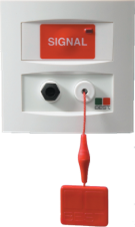
\includegraphics[scale=0.7]{anropspanel.png}
                \caption{Anropspanel}
                \label{anropspanel}
        \end{subfigure}%
        \begin{subfigure}[b]{0.3\textwidth}
        		\centering
                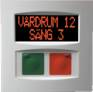
\includegraphics[scale=1.5]{rompanel.jpg}
                \caption{Rompanel}
                \label{rompanel}
        \end{subfigure}
        \begin{subfigure}[b]{0.3\textwidth}
        		\centering
                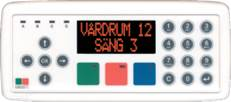
\includegraphics[scale=1]{vaktromsapparat.jpg}
                \caption{Vaktromsapparat}
                \label{vaktromsapparat}
        \end{subfigure}
        \caption{Pasientsignalanlegget}
        \label{pasientsignalanlegget}
\end{figure}

\noindent
\subsubsection{Anropspanelet}
Det finnes to typer anropspanel, et for våtrom og et for vanlig rom. I vanlige sengerom er anropspanelet plassert ved sengen, og har en trykknapp med lysdiode og en trekksnor.
Trykknappen utløser et hasteanrop, mens trekksnoren utløser et pasientsignal.

\subsubsection{Rompanelet}
Rompanelet er plassert ved døren til hvert av sengerommene på tunet. Det har et display, og en grønn og en rød trykknapp med hver sin lysdiode. Grønn knapp trykkes for å markere pleiepersonells tilstedeværelse eller for å avstille et signal. Rød knapp trykkes for å utløse pasientsignal, eller et hasteanrop dersom tilstedemarkering er aktivert. Rød knapp kan også holdes inne i 2 sekunder for å utløse hasteanrop, dersom tilstedemarkering ikke er aktivert. 

\subsubsection{Vaktromsapparatet}
Vaktromsapparatet er sentralt plassert i det åpne landskapet på sengetunet. Det består av et display og flere tall- og tegntaster. Displayet indikerer stedangivelse for et pasientsignal, hasteanrop og tilstedemarkerte rom. Pasientsignaler og hasteanrop er signalisert med rød tekst, mens tilstedemarkering er vist ved grønn tekst. Tall- og tegntastene brukes for å programmere apparatet.

\subsection{Det trådløse systemet}
Pasientsignalanlegget er videre tilkoblet det trådløse systemet, som består av følgende IKT-komponenter: pasientsignalapplikasjon, trådløs telefonenhet og pasientterminal, illustrert i figur \ref{pasientapplikasjon}, \ref{telefonenhet} og \ref{pasientterminal} henholdsvis.

\begin{figure}[H]
        \centering
        \begin{subfigure}[b]{0.35\textwidth}
        		\centering
                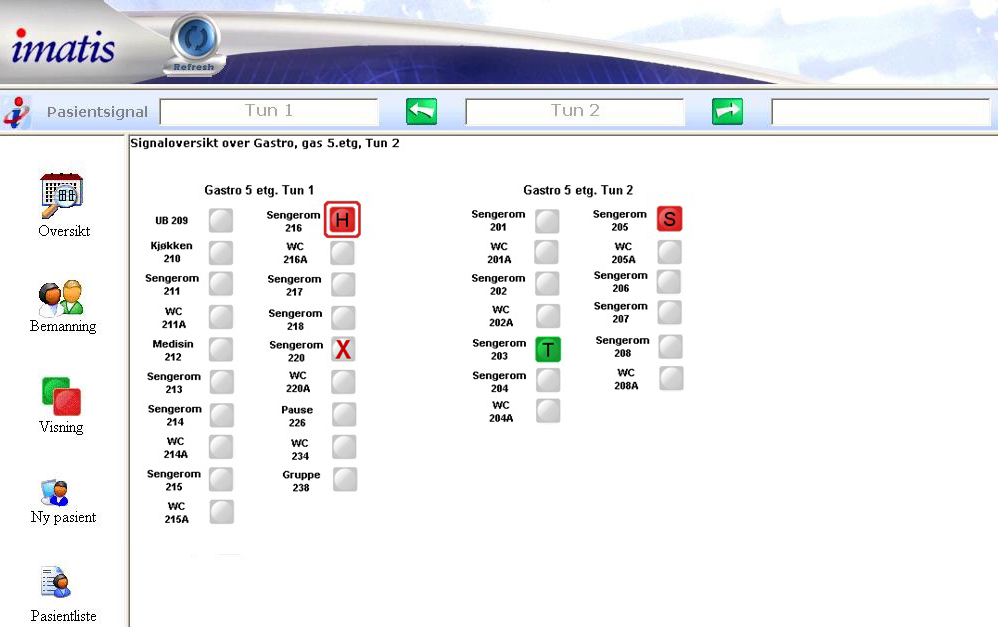
\includegraphics[scale=0.2]{pasientapplikasjon.jpg}
                \caption{Pasientsignalapplikasjon}
                \label{pasientapplikasjon}
        \end{subfigure}
        \begin{subfigure}[b]{0.35\textwidth}
        		\centering
                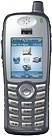
\includegraphics[scale=1]{telefon.jpg}
                \caption{Trådløs telefonenhet}
                \label{telefonenhet}
        \end{subfigure}
        \begin{subfigure}[b]{0.25\textwidth}
        		\centering
                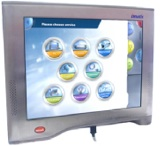
\includegraphics[scale=0.4]{pasientterminal.jpg}
                \caption{Pasientterminal}
                \label{pasientterminal}
        \end{subfigure}
        \caption{Det trådløse systemet}\label{dettradlosesystemet}
\end{figure}

\subsubsection{Pasientsignalapplikasjon}
Pasientsignalapplikasjonen kjører på en PC på hvert sengetun, 24 timer i døgnet, hver dag. Applikasjonen tilbyr i hovedsak fem funksjoner: (1) oversikt, (2) bemanning, (3) visning, (4) registrering av ny pasient og (5) en pasientliste. Vi vil her utdype funksjonene bemanning og visning, da disse er av mest relevans for vår oppgave.  

\noindent
Bemanningsplanen, vist i figur \ref{bemanningsplan}, knytter tilgjengelig pleiepersonell til rommene ved et sengetun. Pasientsignalene vil dermed sendes til riktig mottaker på bakgrunn av bemanningsplanen. For hvert rom vil det normalt tilknyttes en primærsykepleier og en disponibel sykepleier.

\begin{figure}[H]
\centering
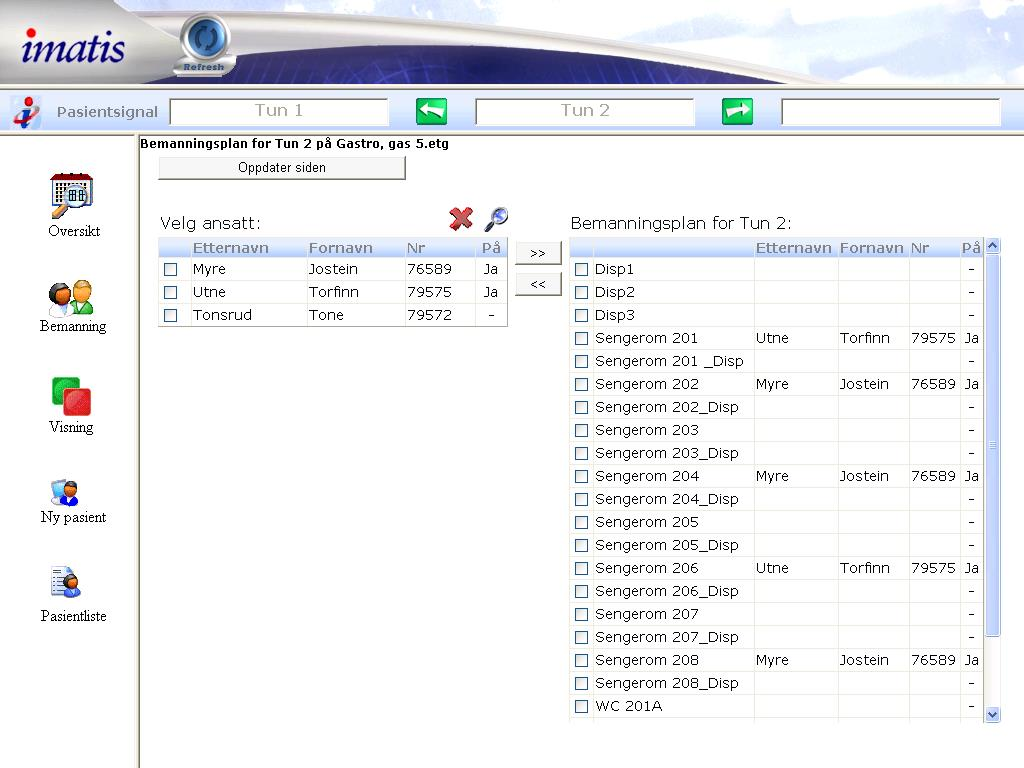
\includegraphics[scale=0.4]{bemanningsplan.jpg}
\caption{Bemanningsplan}
\label{bemanningsplan}
\end{figure}

\noindent
Funksjonen visning, vist i figur \ref{visning}, viser en oversikt over pasientsignalanlegget ved gjeldende sengetun, her vist som Gastro i 5. etasje, tun en og to. Grønn T markerer at pleiepersonell har trykket på den grønne knappen på rompanelet i det gjeldende sengerommet, og tilsynelatende er tilstede. Dette er ikke nødvendigvis riktig, da pleiepersonell kan glemme å trykke av den grønne knappen da de forlater rommet. Rød S signaliserer et pasientsignal, mens innrammet rød H signaliserer et hasteanrop. Rødt kryss varsler feil i systemet.

\begin{figure}[H]
\centering
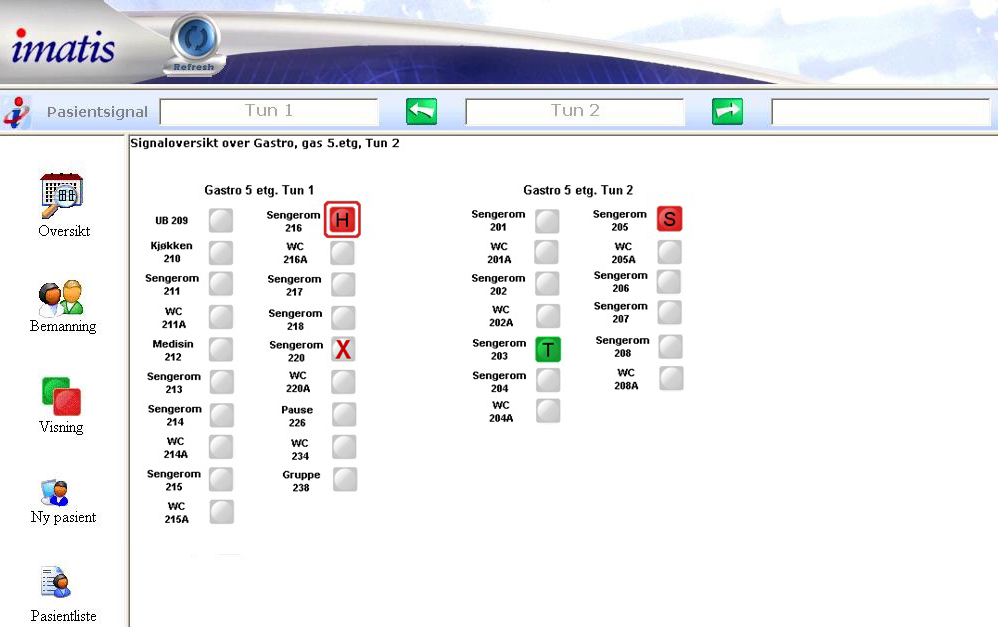
\includegraphics[scale=0.4]{pasientapplikasjon.jpg}
\caption{Visning}
\label{visning}
\end{figure}

\subsubsection{Trådløs telefonenhet}
De trådløse telefonenhetene inngår i det IP-baserte telefonisystemet ved St. Olavs Hospital, og er av typen Cisco Wireless IP Phone 7921G. I tillegg til å tilby basisfunksjoner som å ringe og sende tekstmeldinger, støtter de tjenester for alarmering. Pleiepersonell logger seg på telefonene for å motta pasientsignal og hasteanrop i forhold til ansvar gitt i bemanningsplanen.

\subsubsection{Pasientterminal}
Pasientterminalen inneholder en rekke funksjoner som pasienten kan benytte seg av, deriblant TV, radio, telefon, internett, spill og knapp for pasientsignal. Den røde knappen under skjermen benyttes for å utløse pasientsignal, og denne fungerer uavhengig av om terminalen er skrudd på eller ikke.

\pagebreak

\subsection{Hvordan det hele henger sammen}
\begin{figure}[H]
\centering
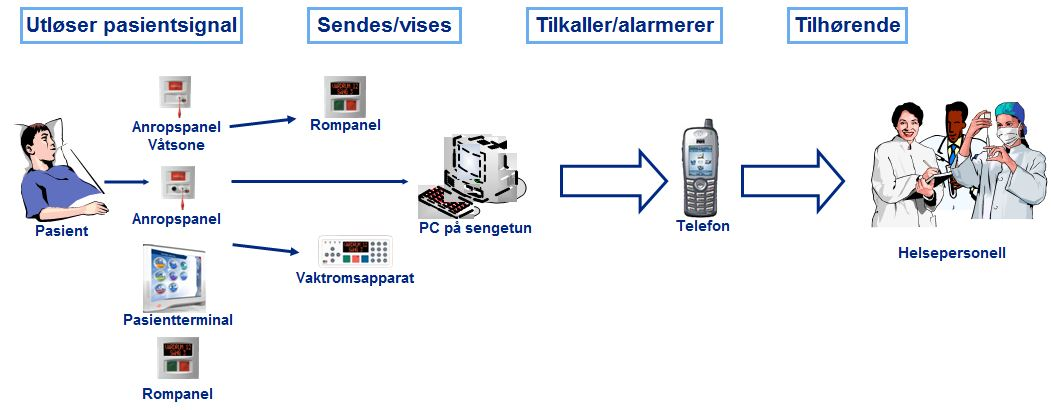
\includegraphics[scale=0.5]{alarmprosess.jpg}
\caption{Pasientsignal (delvis modifisert)}
\label{alarmprosess}
\end{figure}

\noindent
Pasienten kan utløse et pasientsignal ved å trykke på signalknappen på pasientterminalen, dra i snoren på anropspanelet, eller trykke på den røde knappen på rompanelet. Da vil lysdioden på rompanelet og anropspanelet blinke rødt. På andre sengerom hvor tilstedemarkering er aktivert vil lysdioden blinke rødt, og nummer- og stedsangivelse vil vises på displayet. Vaktromsapparatet vil blinke og avgi lydsignal, og pasientsignalapplikasjonen viser markering for pasientsignal.

\begin{figure}[H]
        \centering
        \begin{subfigure}[b]{0.35\textwidth}
        		\centering
                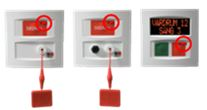
\includegraphics[scale=0.7]{signal_paneler.jpg}
        \end{subfigure}
        \begin{subfigure}[b]{0.35\textwidth}
        		\centering
                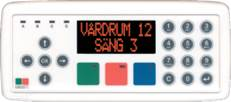
\includegraphics[scale=1]{vaktromsapparat.jpg}
                \label{telefon}
        \end{subfigure}
        \caption{Alarmering ved pasientsignal}\label{pasientsignalalarm}
\end{figure}

\begin{figure}[H]
\centering
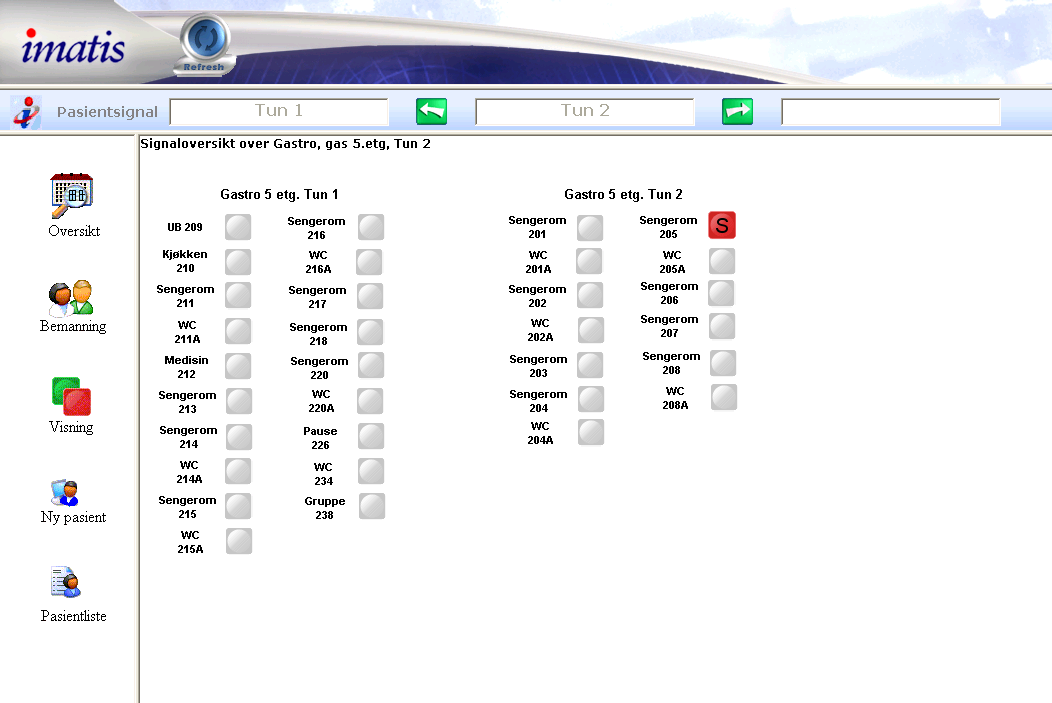
\includegraphics[scale=0.4]{applikasjonalarm.png}
\caption{Pasientsignalapplikasjon ved alarm (Brukermanual for Pasientsignal og Pasientsignalapplikasjon )}
\label{alarmprosess}
\end{figure}

\noindent
Dedikert pleiepersonell registrert i bemanningsplanen tilkalles på sin trådløse telefonenhet ved at melding vises på displayet, og lydsignal avgis. Mottaker har da mulighet til å godta eller avvise pasientsignalet. Dersom vedkommende velger å avvise tilkallingen, eller ikke foretar seg noe innen 15 sekunder, vil signalet sendes videre til neste ressurs. Slik vil det fortsette inntil tilkallingen blir bekreftet.

\begin{figure}[H]
\centering
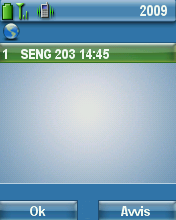
\includegraphics[scale=1]{alarmtelefon.png}
\caption{Trådløs telefonenhet ved alarm}
\label{alarmprosess}
\end{figure}

\noindent
Dersom mottaker godtar tilkallingen vil den legges i mottakers arbeidsliste, og vedkommende har 2 minutter på seg for å tilstedemarkere seg på rommet, ellers vil tilkallingen videresendes til neste registrerte ressurs.

\begin{figure}[H]
\centering
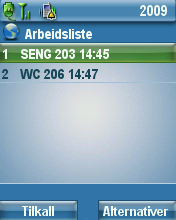
\includegraphics[scale=1]{telefonok.png}
\caption{Arbeidsliste}
\label{alarmprosess}
\end{figure}

\noindent
Ved tilstedemarkering vil lyssignalet stoppe på anropspanelene, og rompanelet vil blinke med grønt lys. Vaktromsapparatet viser sengenummer og stopper lydsignalet, tilkallingen fjernes fra mottakers arbeidsliste, og pasientsignalapplikasjonen viser tilstedemarkering.
 
\begin{figure}[H]
        \centering
        \begin{subfigure}[b]{0.35\textwidth}
        		\centering
                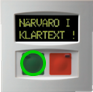
\includegraphics[scale=1]{rompanelok.png}
                \caption{Rompanel}
                \label{rompanelok}
        \end{subfigure}
        \begin{subfigure}[b]{0.25\textwidth}
        		\centering
                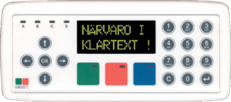
\includegraphics[scale=0.9]{vaok.png}
                \caption{Vaktromsapparat}
                \label{vaok}
        \end{subfigure}
        \caption{Det faste systemet etter tilstedemarkering}
\end{figure} 

\begin{figure}[H]
\centering
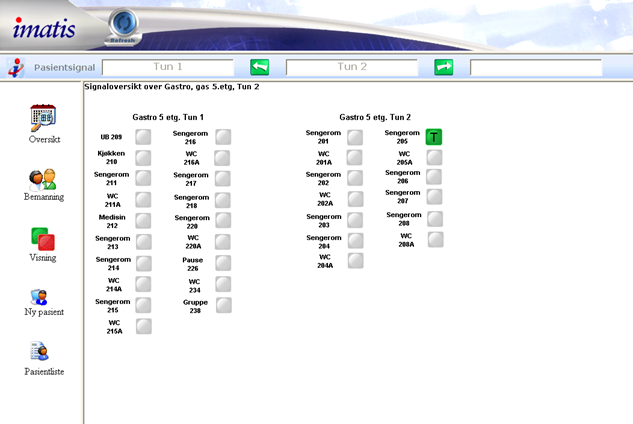
\includegraphics[scale=1]{applikasjonok.png}
\caption{Pasientsignalapplikasjon etter tilstedemarkering}
\label{applikasjonok}
\end{figure}

\noindent
Pleiepersonell trykker på den grønne knappen for å avstille pasientsignalet. Dersom pleiepersonell får behov for assistanse kan han/hun utløse et hasteanrop ved å bruke signalknappen på anropspanelet eller den røde knappen på rompanelet. Alarmen indikeres ved et hastig lydsignal, og røde tall for romnummer og stedsangivelse blinker hurtig på vaktromsapparatet og tilstedemarkerte rompaneler. På det gjeldende rommet vil både rød og grønn lysdiode blinke på rompanelet. I tillegg sendes en hasteanropsmelding, som ikke kan avvises, til samtlige av pleiepersonellets trådløse telefoner på sengetunet. Pasientsignalapplikasjonen viser markering for hasteanrop. Hasteanrop legges i arbeidsliste og avstilles på samme måte som pasientsignaler.

\begin{figure}[H]
\centering
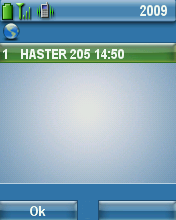
\includegraphics[scale=1]{hasteanropsmelding.png}
\caption{Trådløs telefonenhet ved hasteanrop}

\begin{figure}[H]
\centering
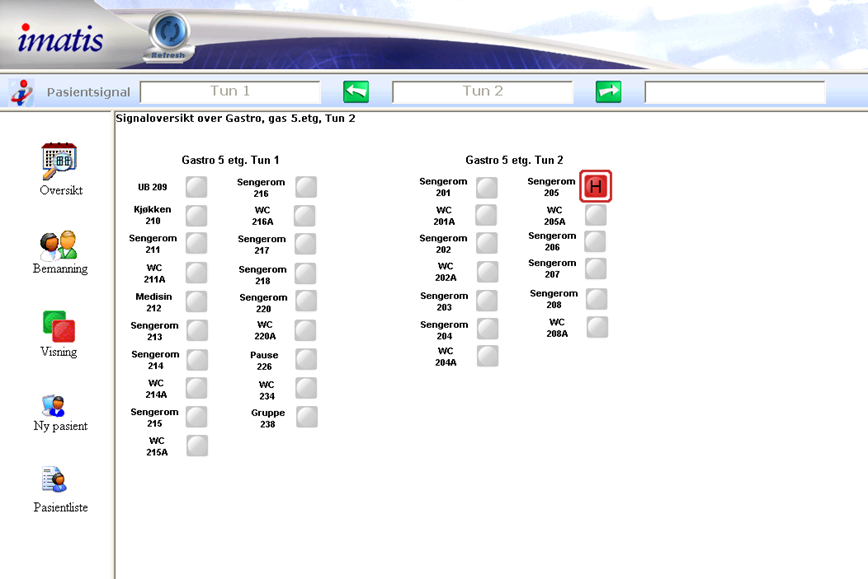
\includegraphics[scale=1]{applikasjonhast.png}
\caption{Pasientsignalapplikasjon ved hasteanrop}
\label{applikasjonok}
\end{figure}
\label{applikasjonok}
\end{figure}












\end{document} 
